%%% Time-stamp: <2015-04-15 00:55:14 sunthar>

%%% $Log:$

%\documentclass[11pt,a4paper,openright]{report}
\documentclass[seminar,twoside]{iitbreport}


%% Selectively comment out sections that you want to be left out but
%% maintaining the page numbers and other \ref
\includeonly{%
  declaration,
  certificate,
  acknowledgement,
  intro/introduction,
  lit/literature,
  methods/methods,
  Navier-Stokes/ns,
  expt/experimental_aps1,
  Multigrid/multigrid,
  surface_tension/surface_tension,
}

%%% Some commonly used packages (make sure your LaTeX installation
%%% contains these packages, if not ask your senior to help installing
%%% the packages)


\usepackage{booktabs}
\graphicspath{{images/},{images2/},{images3/},{Multigrid/}}
\usepackage{subfig}
\usepackage{tabularx}
\usepackage{caption}
\usepackage{enumitem}
\usepackage{float}
\usepackage{algorithm}
 \usepackage{algpseudocode}
\setlist{nosep} % or \setlist{noitemsep} to leave space around whole list
%%% Macro definitionfor Commonly used symbols

\usepackage[compact]{titlesec}
\usepackage{hyperref}
\raggedbottom

\usepackage{xcolor,colortbl}
\newcommand{\mc}[2]{\multicolumn{#1}{c}{#2}}
\definecolor{Gray}{gray}{0.85}
\newcolumntype{a}{>{\columncolor{Gray}}c}

\usepackage{wrapfig}
\usepackage{framed}


\newcommand{\etas}{\ensuremath{\eta_{\mathrm{s}}}}
\newcommand{\Rey}{\ensuremath{\mathrm{Re}}}	
\newcommand{\avg}[1]{\ensuremath{\overline{#1}}}
\newcommand{\tenpow}[1]{\ensuremath{\times 10^{#1}}}

\newcommand{\pder}[2]{\ensuremath{\frac{\partial#1}{\partial#2}}}


% Referencing macros
\newcommand{\Eqref}[1]{Equation~\eqref{#1}}
\newcommand{\Tabref}[1]{Table~\ref{#1}}
\newcommand{\Figref}[1]{Figure~\ref{#1}}
\newcommand{\Appref}[1]{Appendix~\ref{#1}}



\begin{document}
\pagenumbering{gobble}
\title{Waves and Oscillatons in Fluids}
\author{Palas Kumar Farsoiya \\ (Roll No: 144026002 )}
%\date{\today}
\degree{Doctor of Philosophy}
\dept{Chemical Engineering}
\monthyear{August 2016}

%\makecoverpage
\maketitle
\begin{center}
\textbf{\large Declaration} 
\end{center}
\indent \\
\indent This is to certify that the annual progress seminar report titled \textbf{Waves and Oscillation in Fluids}  which is submitted by me in partial fulfillment of the 
requirement for the award of Ph.D. (\textit{philosophiae doctor}) to Department of Chemical Engineering, IIT Bombay, Mumbai comprises the work carried out by me and
due acknowledgment has been made whenever the work described is based on the findings of other investigators.

\vspace*{1.6cm}

\begin{flushleft}
\underline{\hspace{4cm}}\\
Palas Kumar Farsoiya\\
\end{flushleft}

\begin{center}
\underline{\textbf{\large ACCEPTANCE CERTIFICATE}} \\[1cm]
Seminar Report \\[0.2cm]
Department of Chemical Engineering \\
Indian Institute of Technology, Bombay \\[7.5mm]
\end{center}
%\vspace*{0.75cm}
The Seminar report titled \textbf{Droplet Impact Dynamics} submitted by Palas Kumar Farsoiya (Roll No. 144026002) may please be accepted for being evaluated.\\[1cm]
%\vspace*{1cm}
%\begin{flushright}
\underline{\hspace{4cm}}\\
Prof. Ratul Dasgupta\\
(Research Supervisor)
%\end{flushright}

\begin{center}
\textbf{\large Acknowledgement} 
\end{center}
\indent \\
\indent I would like to acknowledge my supervisor Prof. Ratul Dasgupta for providing me VOF code for further developement. Further, he has appreciated me in developing concepts and manifesting them in codes. He has time to time monitored my progress and provided with valuable aids in terms of suggestions, resources, lectures and even disagreement. His efforts have enormously benefited me.\\
\indent I would also like to thank all my friends and lab mates for providing their valuable insights, friendly guidance and support whenever required. I would like to acknowledge Manoj (Doctoral student, IIT Hyderabad) to help me in Gerris simulations.\\
\indent My wonderful family, which has been my constant source of motivation and inspiration. \\
\\
\\
\indent
Thank you
\vspace*{1.6cm}

%\begin{flushright}
Palas Kumar Farsoiya\\
\indent (124020001)
%\end{flushright}

\begin{abstract}
%  Droplet impingement is a very common phenomenon in the world, natural and man-made around us. 
%  Droplets are formed through instabilities such as Rayleigh-Plateau instability, but their interactions usually with other droplets, and their impingement dynamics on a
%  rigid wall are complex processes which intrigue physicists, mathematicians and engineers. For physicists the interest lies in understanding the solution of the Navier-stokes
%  equation before and after impact and various intricacies of the boundary conditions on dry rigid surfaces. Mathematicians study the asymptotic solution of the governing laws
%  of the fluid dynamics while for engineers, droplet impact is of tremendous technological importance as there are various applications e.g. silicon chip technology, ink jet printing,
%  internal combustion engines, spray painting and coating, plasma spraying and pesticide spraying on crops. \par This report begins with a short literature review of droplet impact. A detailed summary
% of progress made in developing an in-house code capable of modelling two-phase flow is presented accompanied by benchmark results. Experimental results obtained from scientific literature
% are then compared with simulations conducted using an open source code Gerris, for droplet impact on super-hydrophobic surfaces. We conclude by defining broad areas that we plan to study. 
\end{abstract}

\pagenumbering{roman}
\tableofcontents
\listoftables
\listoffigures

\cleardoublepage
\setcounter{page}{1}
\pagenumbering{arabic}

 %
\chapter{Introduction and Literature Review}
\section{Introduction}
Droplet impact is a phenomenon which is prevalent in many industrial processes such ink-jet printing, 
spray cooling of hot surfaces. Microelectronic industries uses precision solder drop dispensing to produce
electric circuits. Aircraft and power distribution lines encounter accumulation of ice involving droplet impact.
Natural phenomena such as rain effects the aeration of lakes, seas and oceans. 
Forensic science necessitates development of non-wettable and fully wettable surfaces. Criminalistics involves
reconstructing crime scenes in which it is need to study the stain patterns of blood drops impacting surfaces.
With a rising world population, there is huge rise in agricultural growth and use of pesticides is necessary. Pesticides spray 
on crops is also an application which exhibits droplet impact on the plants where spreading of droplets is necessary. 
\begin{figure}[tbp]
 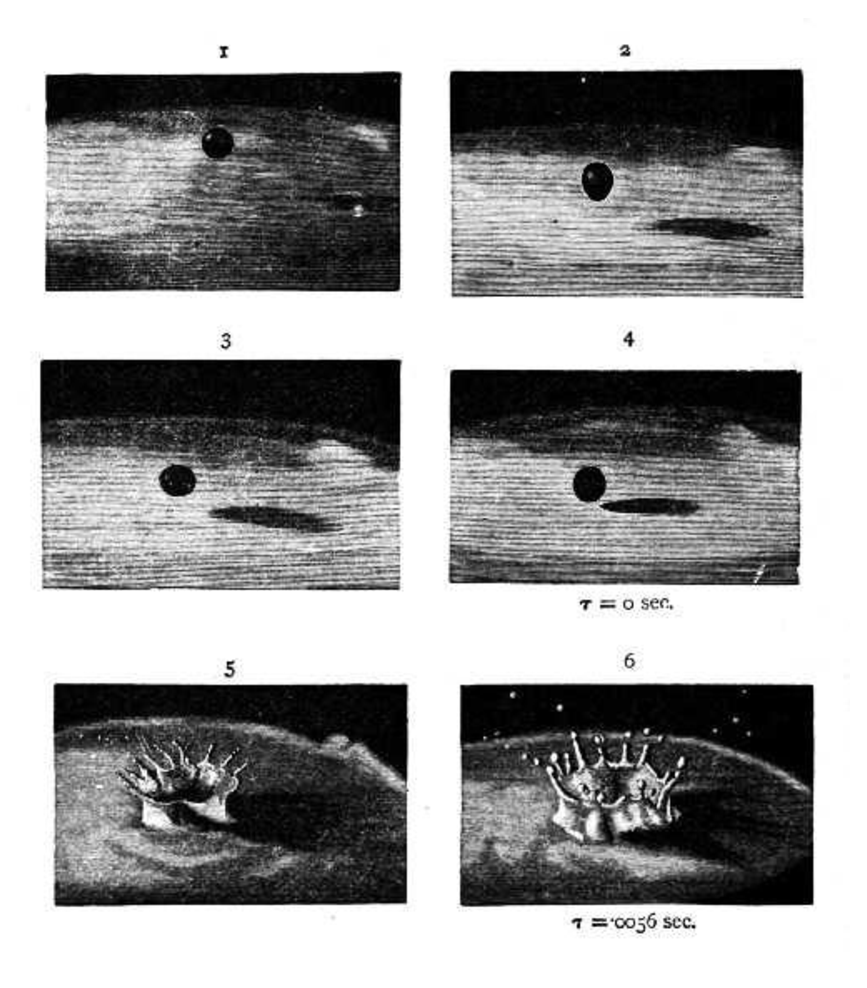
\includegraphics{worthington.eps}
 \caption{Droplet impact graphic by \cite{Worthington1908}}
\label{Fig:Worthington}
\end{figure}


The scientific literature on drops starts with the droplet formation which was studied by many scientists while studying the
free surface flow. The first scientific observation on drops can be found in the book by \cite{Mariotte1700} on motion of  
fluids. They observed that water flowing through the hole of a container bottom breaks into drops. \cite{Taylor1963} solved the  axisymmetric Navier-Stokes  using
singular perturbation method for a drop/bubble in an unbounded fluid. Droplet impact was first investigated experimentally by \cite{Worthington1908} (See Figure \ref{Fig:Worthington}).
The area of droplet formation has also been researched extremely by scientists working in the non-linear dynamics.

The dynamics of the impinging drop is complex and hence many aspects are not understood well. For example, droplets falling
on a surface can undergo many different modes of deformation. It can splash, bounce or simply deposit on a surface. \cite{Rein2002} 
explained through a cartoon, the various possible outcomes of droplet impact. (See Figure \ref{Fig:rein})

\begin{figure}[tbp]
 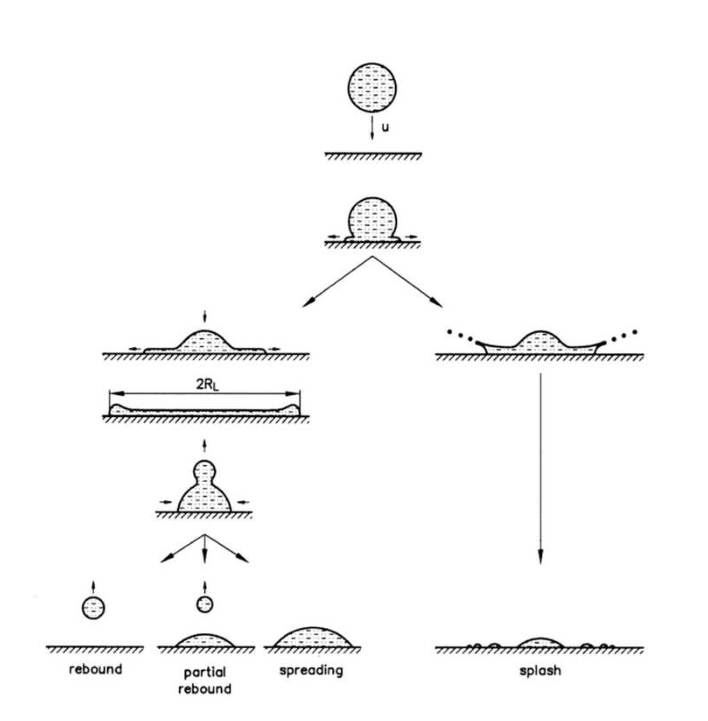
\includegraphics{rein.eps}
 \caption[Different modes of deformation of droplet impact]{Cartoon of different modes of deformation of droplet impact by \cite{Rein2002} }
 \label{Fig:rein}
\end{figure}

 %
\section{Literature Review of droplet impacts}

Droplet impact has been investigated from more than a century.These studies can be classified into three broad categories :- 
\begin{enumerate}
 \item Experimental Phenomenology.
 \item Simulation.
 \item Theory.
\end{enumerate}

There are many studies which are combination of the two or more as well e.g. \cite{Mao1997} has proposed theoretical models which were supported by experiments. We
begin with a brief discussion on experimental phenomenology.
\subsection{Experimental Phenomenology}
With the advent of high speed photography in late 1800s, it became possible to observe numerous phenomena which were too fast for the human eye.
Having developed the skills of high speed photography, \cite{Worthington1908} captured photographs of droplet impact. Since then various aspects of
droplet impact have being studied. There are now sophisticated digital systems which can record images at a very high frame rate 
(See Figure \ref{gunjal}) that enable us to capture very fast dynamics which are not visible to human eye.
\begin{figure}[tbp]
\centering
 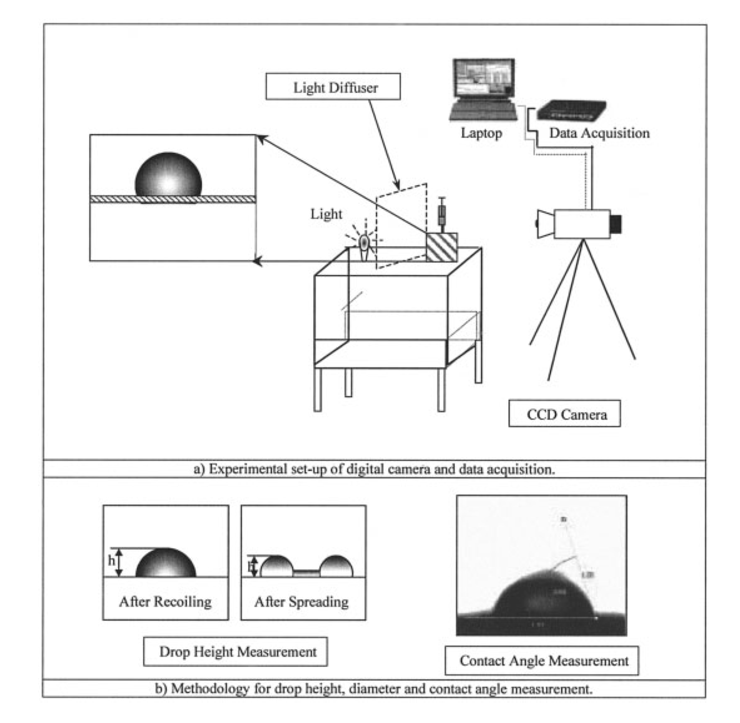
\includegraphics{gunjal.eps}
 \caption[Experimental setup to study droplet impact]{Experimental setup to study droplet impact by \cite{Gunjal2005}}
 \label{gunjal}
\end{figure}
\cite{Richard2000} observed for impact on highly hydrophobic surface (contact angle $ > 170^o$), droplets fully bounce, they 
do not tend to spread (See Figure \ref{richard}). They behaved just like spring but found there was a limit in elasticity due to the transfer
of the part of kinetic energy into the drop vibrations.
\begin{figure}[tbp]
\centering
 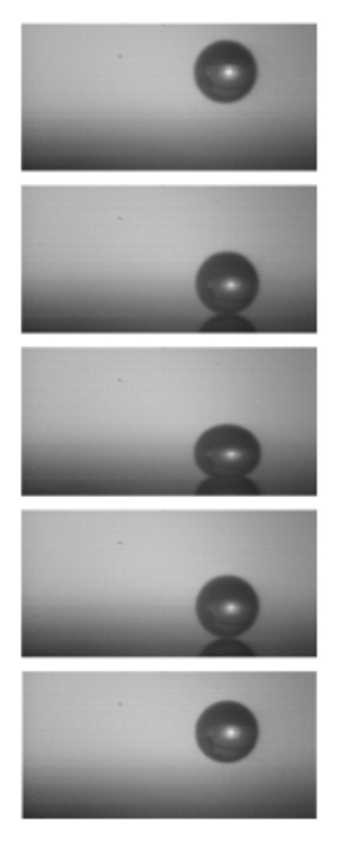
\includegraphics{richard.eps}
 \caption[Droplet impact on superhydrophobic surface]{Droplet impact(R = 0.4 mm) on superhydrophobic surface
 by \cite{Richard2000} }
 \label{richard}
\end{figure}
Droplet impact on dry surfaces are quite different when compared to wet surfaces. \cite{Rioboo2001} studied the effect
various flow parameters and surface characteristics on the droplet impact dynamics. They discovered six different outcomes of a droplet impact on 
a dry surface. In Figure \ref{rioboo} they explained the deposition as droplet deformation and continuous attachment to the surface while spreading without breakup. When
the droplet impacted with a rough surface a splash initiated in the direction of contact line velocity at the onset of spreading called as prompt splash.
Another kind of splash can be seen above the solid surface at the rim of a corona and generally referred to as corona splash.
Sometimes a breakup can be seen while the droplet is receding after maximum spreading, this is attributed to the fact while receding the dynamic contact angle decreases and when 
the limiting value is reached some drops are left behind by the receding lamella. It looks beautiful when a droplet rebounds, this particular process occurs only when a
receding phase  precedes. A full rebound occurs when the dynamic contact angle is large and the receding phases are high in kinetic energy.
\begin{figure}[tbp]
\centering
 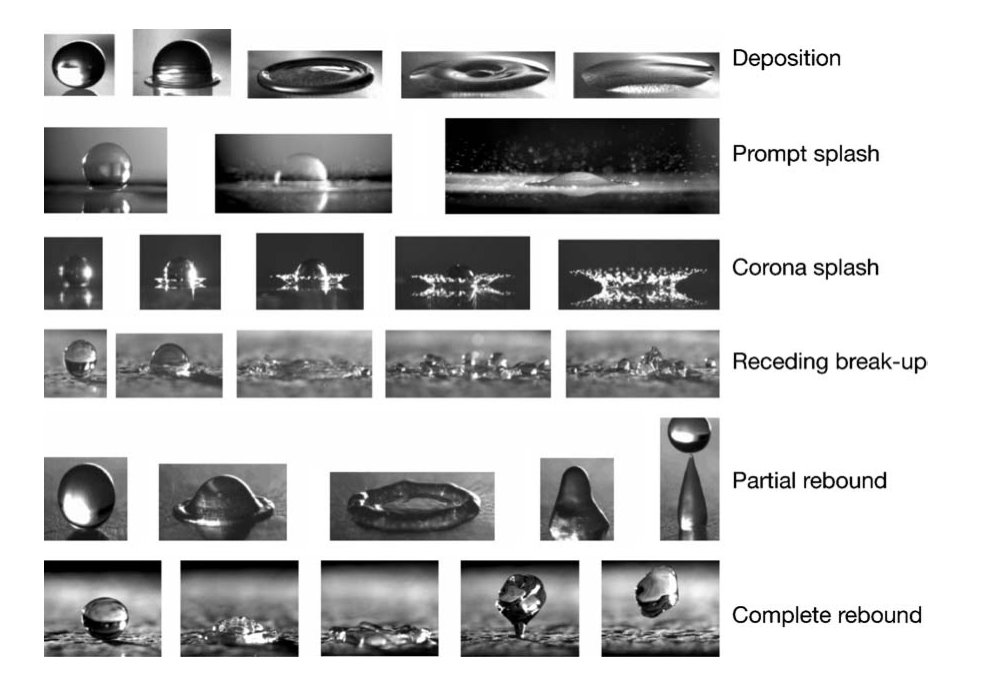
\includegraphics[scale=0.9]{rioboo.eps}
 \caption[Possible outcomes of droplet impact]{Six possible outcomes of droplet impact by \cite{Rioboo2001} }
 \label{rioboo}
\end{figure}
Many scientists have been interested in droplet impact on hydrophobic surfaces. In one such study \cite{Richard2002} found that the contact time of 
bouncing drop does not depend upon the impact velocity of the drop (See Figure \ref{richard2}).
\begin{figure}[tbp]
\centering
 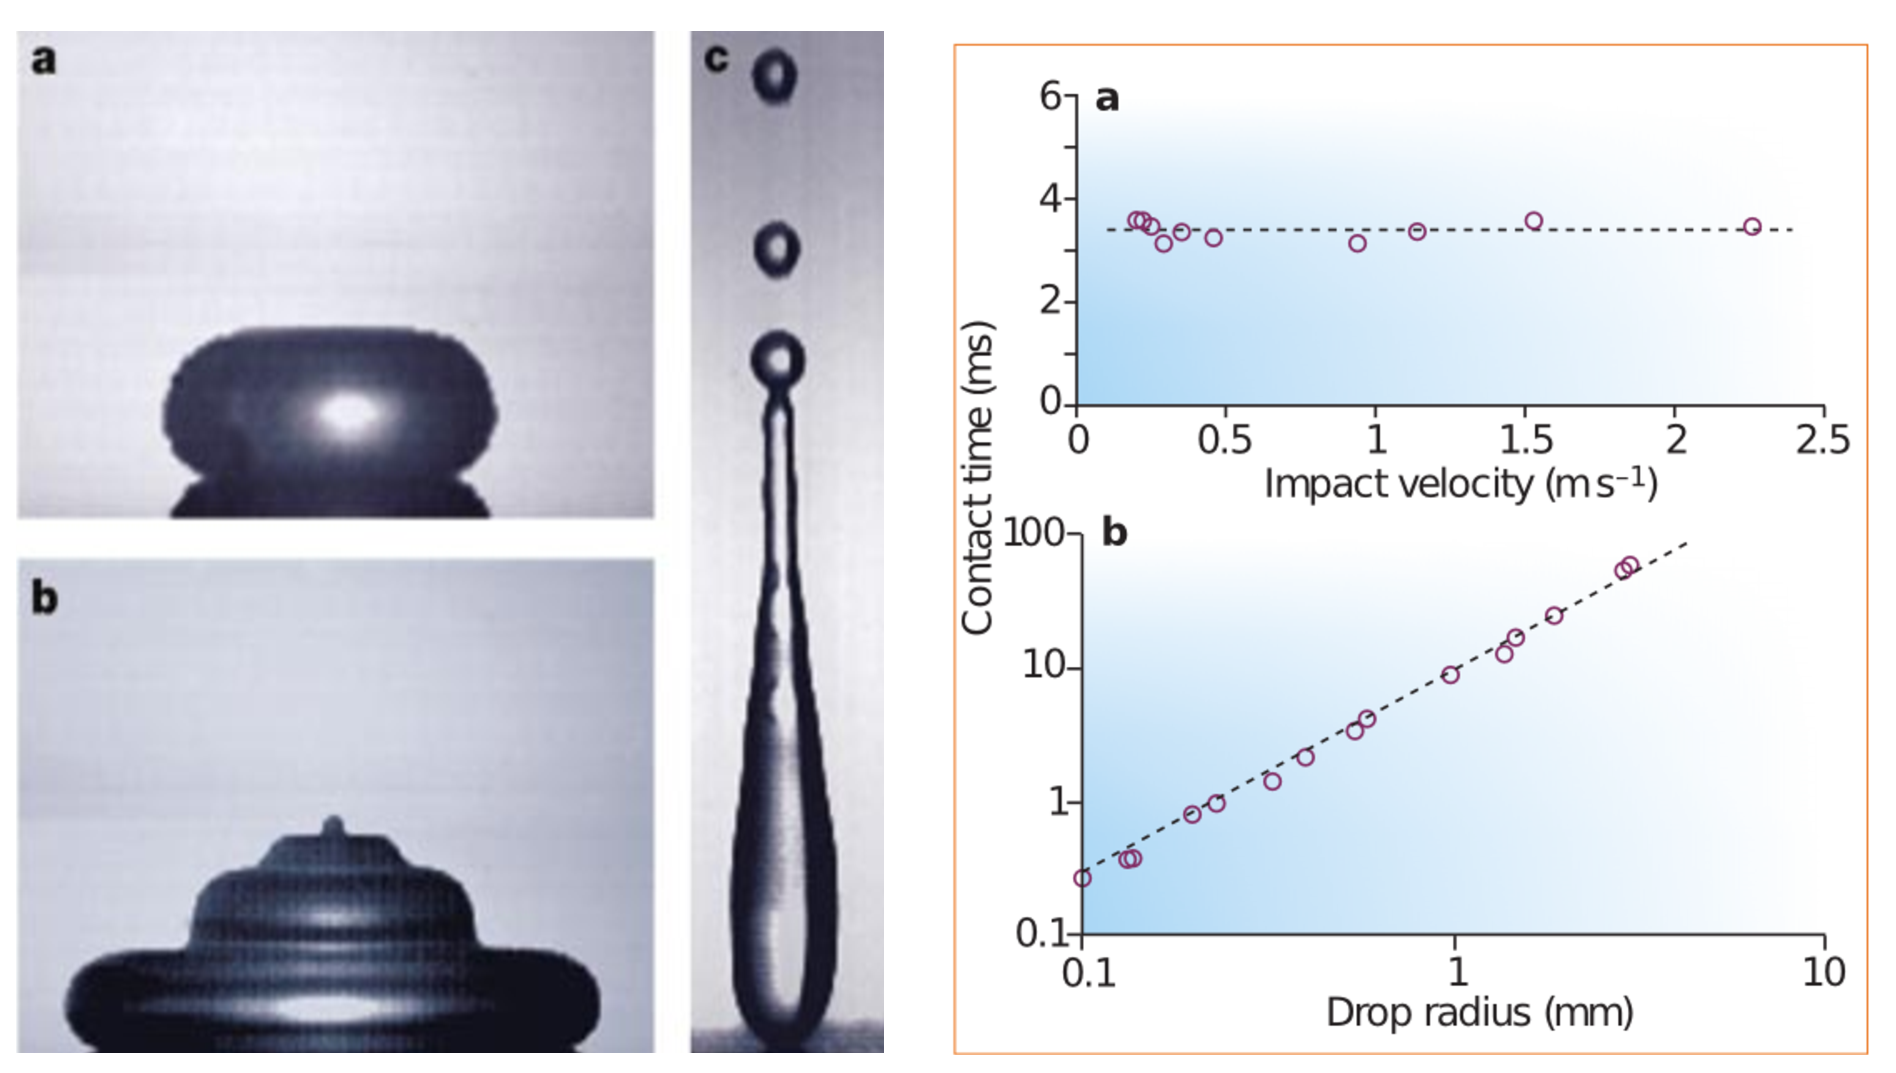
\includegraphics[scale=0.4]{richardc.eps}
 \caption[Contact time of droplet impact on hydrophobic surfaces ]{Contact time of droplet impact on hydrophobic surfaces by \cite{Richard2002} }
 \label{richard2}
\end{figure}
Movement of contact line is a complex phenomena which \cite{Roux2004} studied and obtained an empirical relationship with wetting velocity
of contact line and the impact velocity of the drop. This was later verified by \cite{Hung2011}.
There are a lot of studies on newtonian fluid droplet impact but \cite{Crooks2001} performed some experiments on non-newtonian 
fluids and concluded that the recoil behavior of droplet does not depend on the dynamic surface tension below a critical surfactant
concentration. Here surfactant was added to make the fluid non-newtonian.
\subsection{Simulations}
One of the very early simulation of droplet impact was by \cite{Harlow1967}. They solved the Navier-Stokes equations in cylindrical coordinates in order to
investigate the splash of a drop on a flat plate and deep pool. They used the Marker and Cell {(MAC)} method for interface tracking. The effect of microscopic 
factors such as molecules movement of fluid contact line and surface roughness were also verified by \cite{Gunjal2005} through simulations and experiments. Impact on
inclined surfaces have also received attention in past few years by \cite{Pasandideh1996}, \cite{Kang2000}, \cite{Fukai2000}, \cite{Bussmann1999} and \cite{Sikalo2005}.
These also have been studied by \cite{Lunkad2007} through simulations. \cite{Lunkad2007} applied a Dynamic Contact Angle {(DCA)} model and compared it with Static Contact 
Angle {(SCA)} results, and recommended   {(DCA)} for numerical simulations for better results.

\begin{figure}[tbp]
\centering
 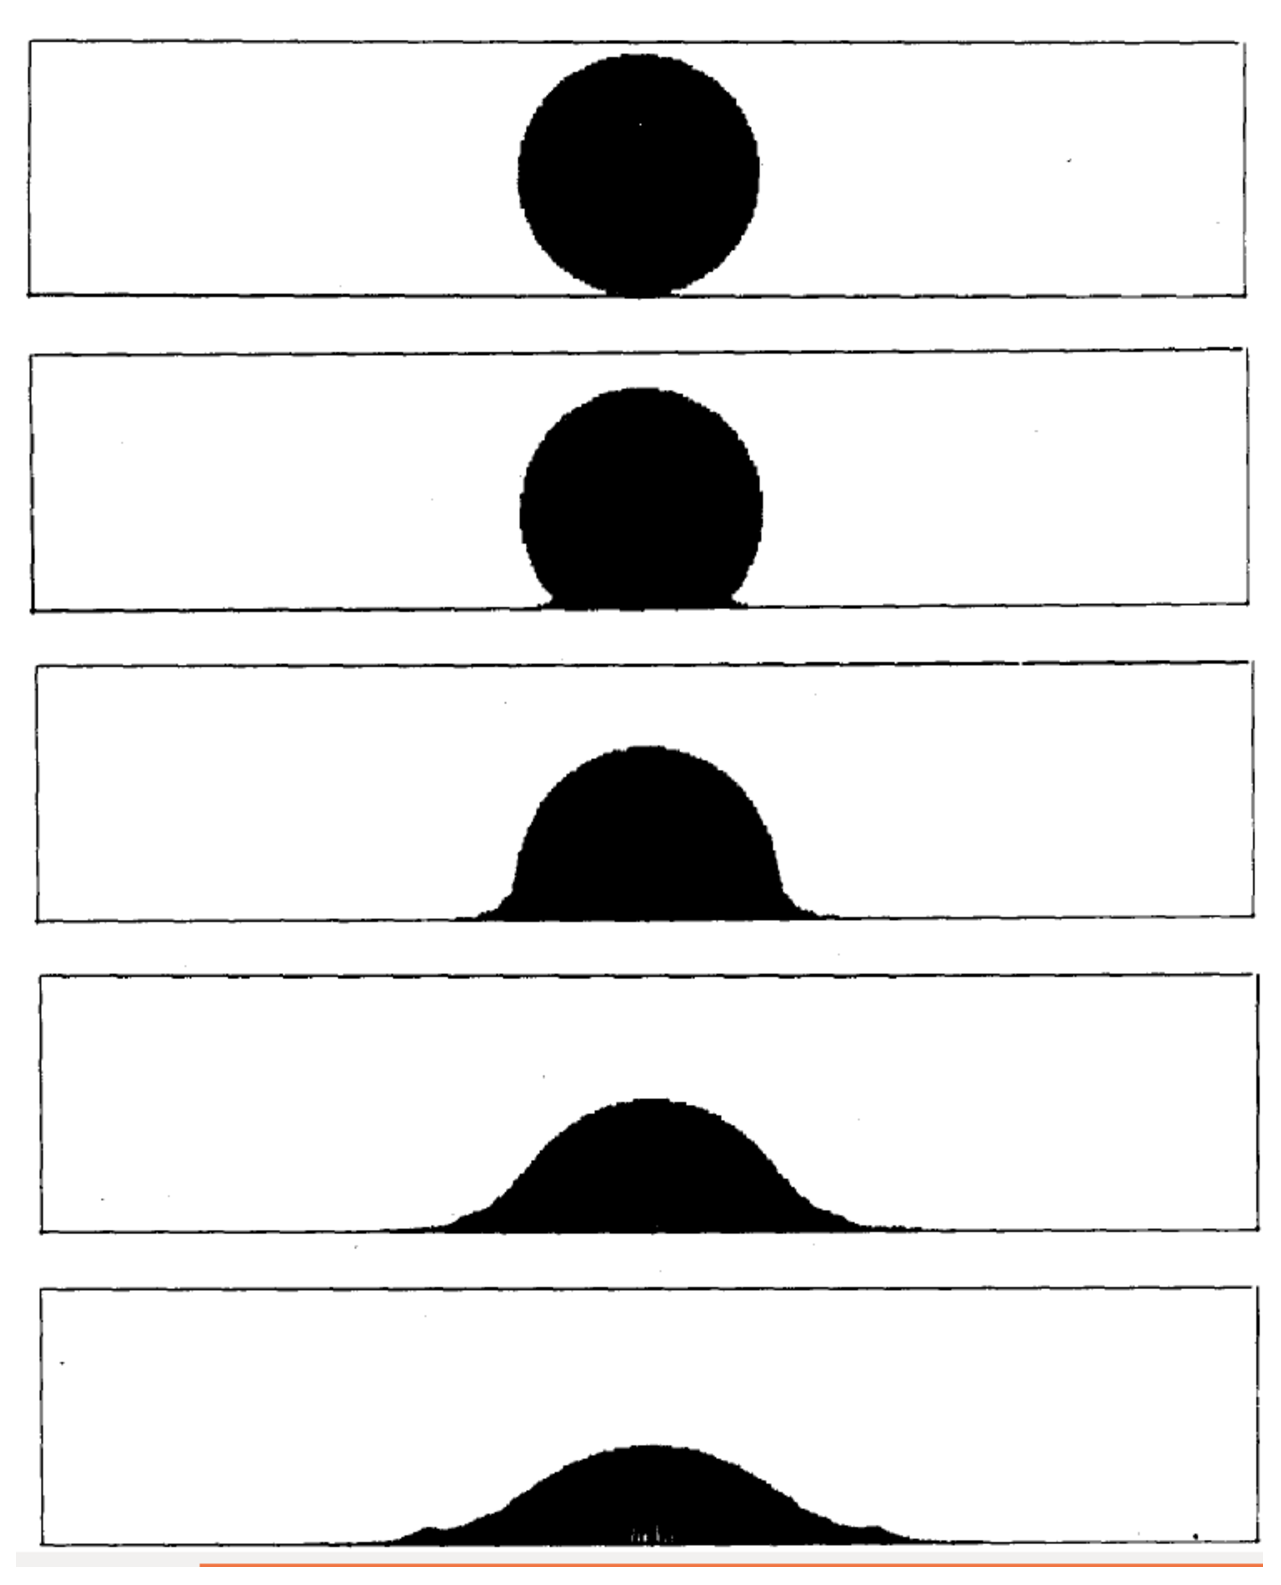
\includegraphics[scale=0.4]{harlow.eps}
 \caption[First numerical study on droplet impact]{The very first numerical study of droplet 
 impact (Reproduced by \cite{Harlow1967} under fair usage policy)}
\end{figure}

\subsection{Theory}
There have been many attempts to explain and model some phenomena which occurs during droplet impact such as 
spread of the droplet after impact. These have been investigated by \cite{Madejski1976}, \cite{Jones1971}, \cite{Chandra1991}, \cite{Scheller1995}, \cite{Bennett1993}, \cite{Pasandideh1996}.
A model was proposed by \cite{Mao1997} for maximum spread as a function of 
 Weber number, Reynolds number, and static contact angle. They also derived a model to predict the rebound by applying conservation of energy, as a function of 
 static contact angle and maximum spread diameter.
Recently a remarkable study by \cite {Liu2015} explained the splashing of droplet on smooth surfaces being due to Kelvin-Helmholtz instability in ultra-thin layer of 
air between the droplet and the surface (See Figure \ref{Fig:liu}).
\begin{figure}
 \centering
 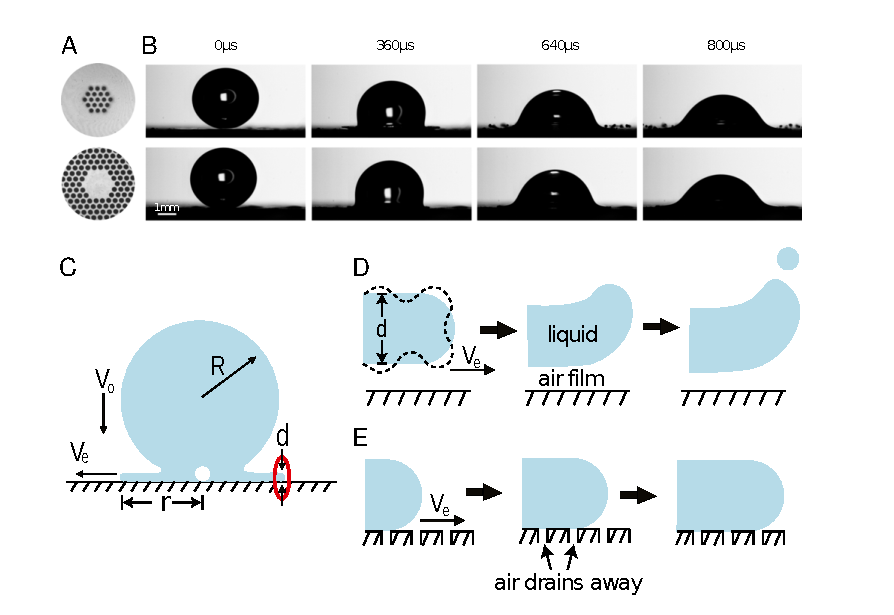
\includegraphics{Liu2015.eps}
 \caption[Kelvin-Helmholtz instability in a droplet splash]{Graphics verifying and explaining the KH instability in the droplet impact which initiates splash (Reproduced by \cite{Liu2015} under fair usage policy)}
 \label{Fig:liu}
\end{figure}

\section{Discussion}
The simulation droplet impact is a complex study as the multiphase solvers must take the effect of surface into the solution. The boundary conditions at the impact surface are non trivial. It
requires understanding of moving contact lines and dynamic contact angles which then has to be implemented in the numerical study. Droplet impact on superhydrophobic surfaces 
however are simpler to study because of the negligible effect of contact line.


 \chapter{Volume of Fluid method}

\section{Introduction}
In this chapter we present the development of in-house code for simulating a two phase flow.
Mathematicians and physicists have studied the dynamics of multiphase flows and as discussed in the previous chapter
literature is quite extensive. Governing equations for such flows are not only nonlinear but the 
position of the interface needs to be found out as a part of solution. Consequently, analytical solutions exist only for very simple problems such as oscillations of bubbles and droplets,
inviscid linear waves and steady state motion of bubbles and droplets in Stokes flow. Thus there is a need for numerical solutions been felt by the multiphase
research community since late fifties and early sixties. 
\cite{Hirt1981} came up with the idea of Volume of Fluid interface {(VOF)} tracking to approximate
the free boundaries in numerical simulations. This method is based on a concept of fractional volume of fluid. This is still widely used due to its flexibility and efficiency
compared to other methods. 
The volume of fluid method conserves mass up to machine accuracy, level set methods conventionally have some issues of mass conservation but
are better in the reconstruction of curved interfaces and thus easier for implementation of surface tension.

\section{The Volume of Fluid method}
This method starts with defining a quantity called as volume fraction F, for each cell in the computational domain. For a binary phase system there is a dark fluid and light fluid.
F is the ratio of volume of the dark fluid to the volume of the cell itself. The cells with only light fluid are chosen to have F = 0 and whereas those with only dark fluid F = 1. For interfacial cells
F will have a value between 0 and 1. The volume of fluid when advected does not change with respect to the fluid parcel. Hence, it satisfies the following relation,

\begin{eqnarray}
\frac{D F}{D t} = 0 
\end{eqnarray}

The Eulerian form would be,

\begin{eqnarray}
 \frac{\partial F}{\partial t}+( u. \nabla)F=0
 \label{Eq:advection_vof}
\end{eqnarray}



As interface in Volume of fluid method can be reconstructed in many ways we choose the Least Squares Volume of 
Fluid Reconstruction Algorithm proposed by \cite{Pilliod2004} which is one of the most accurate algorithm available in literature. It is second order accurate in space 
and can be extended to the 3D. It represents the interface as a line in 2D and a plane in 3D. The VOF method achieves higher accuracy using geometrical techniques to reconstruct
and advect the interface.
Any interface reconstruction algorithm consists two basic steps:-
\begin{enumerate}
 \item Interface Reconstruction
 \item Advection of F field
\end{enumerate}
\pagebreak

\subsection{Interface Reconstruction by Least Squares of Volume of Fluid Interface Reconstruction Algorithm (LVIRA)}
\subsubsection{Step I : Obtain F field}
At first an F-field is obtained by knowing the initial free surface and then by calculating the F values for each cell. 
For reconstruction of interface a cell having a value of F between 0 and 1 is located.

\subsubsection{Step II : Initial guess of slope}
The initial slope of the normal to the interface away from the dark fluid can obtained using (Green-Gauss gradient \cite{Gerlach2006}) which is  given by 
\begin{eqnarray}
  N_x=-\frac{1}{\Delta x}{[F_{r+1,c+1}+2F_{r,c+1}+F_{r-1,c+1}-F_{r+1,c-1}-2F_{r,c-1}-F_{r-1,c-1}]} \\
  N_y=-\frac{1}{\Delta y}{[F_{r+1,c+1}+2F_{r+1,c}+F_{r+1,c-1}-F_{r-1,c+1}-2F_{r-1,c}-F_{r-1,c-1}]}
  \label{Eq:GG}
\end{eqnarray}

\subsubsection{Step III: Quadrant Identification}
To get the interface as a line in 2D, we have to determine its shape and orientation in a cell. First step is to get the normal orientation in the quadrant.
 Signs of $N_x$ and $N_y$ will determine the quadrant in which the normal points away from the dark fluid present in the cell. 
  \begin{figure}%[H]
  \centering
   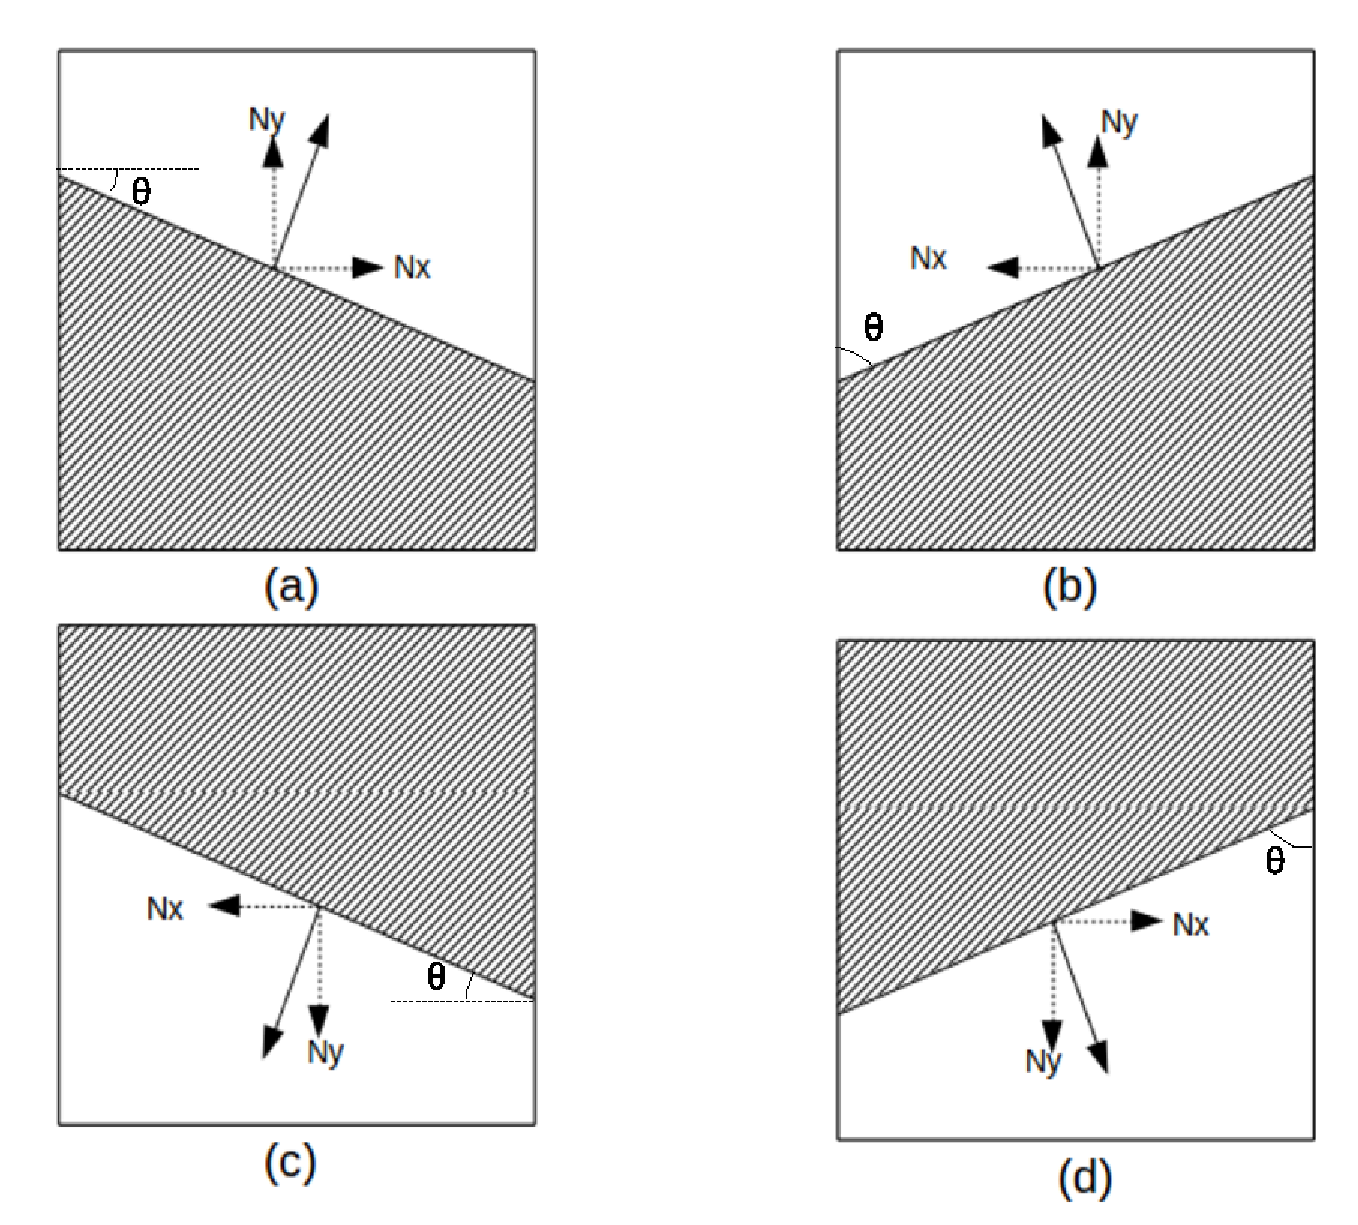
\includegraphics[scale=0.4]{quad.eps}
   \caption[Interface normal direction]{(a)I Quad (b) II Quad (c) III Quad (d) IV Quad }
   \label{Fig:quad}
  \end{figure}

\subsubsection{Step IV: Angle Calculation}
 The angle, $\theta$ is the positive acute angle made by the interface with x-axis if the normal points into first and the third quadrant and positive acute angle made by 
 the interface by y-axis if the normal points into the second and fourth quadrant. This definition is necessary because we treat all other quadrants as the $I^{st}$ quadrant
 by suitable rotation. So for the second and the fourth quadrant $\theta$ has to be redefined. Refer to Figure \ref{Fig:quad} for definition of theta. This is 
 required to do since the algorithm is developed in way it works for normal in first quadrant and all other cases has to be modified according to algorithm.
% 
%  Equation \ref{Eq:angle} gives the expression for calculating $\theta$
% \begin{equation}
%  \theta=\frac{\pi}{2}-tan^{-1}\left(\frac{N_x}{N_y}\right)
%  \label{Eq:angle}
%  \end{equation}
% \begin{wrapfigure}{r}{0.5\textwidth}
%   \begin{center}
%     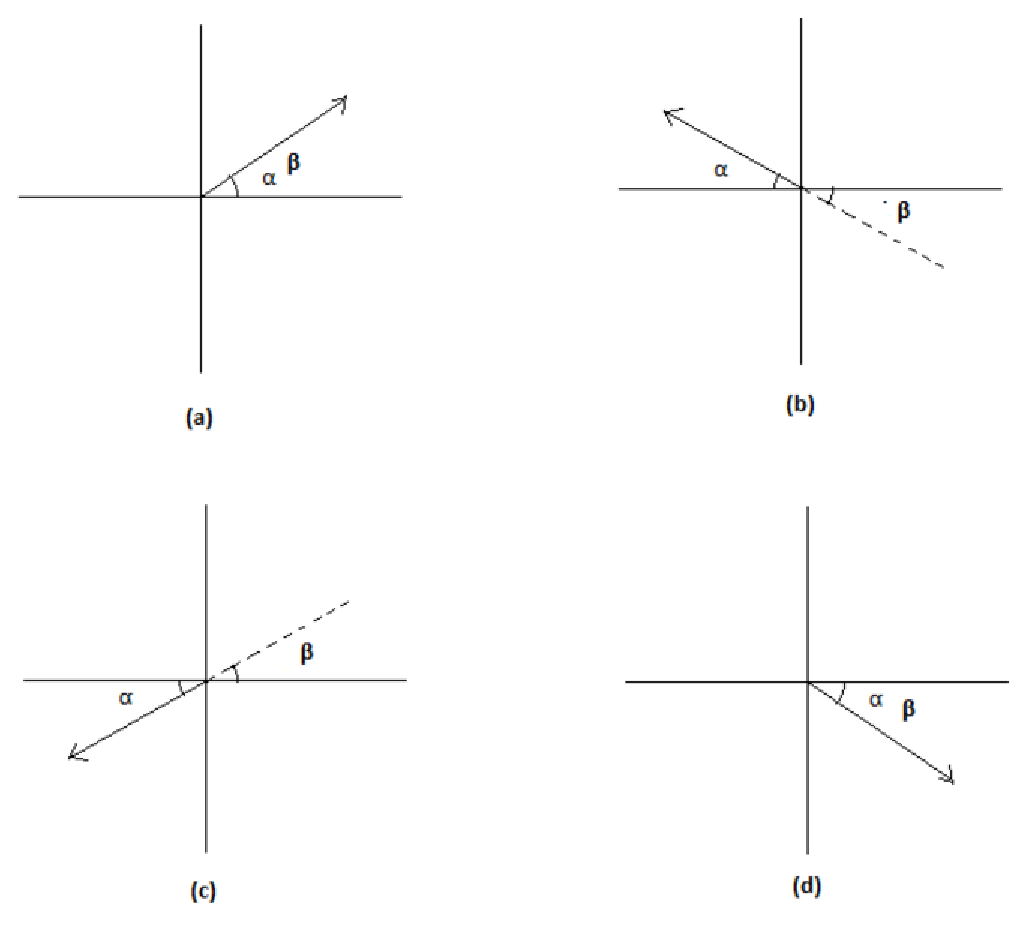
\includegraphics[width=0.48\textwidth]{atan.eps}
%   \end{center}
%   \caption{Angle value returned by gcc compiler}
%     \label{Fig:gcc}
% \end{wrapfigure}
%  
% The function atan() in GCC returns a value between $\frac{-\pi}{2}$ and $\frac{\pi}{2}$ as shown in Figure \ref{Fig:gcc}. The slope, $\frac{N_y}{N_x}$ of normal to interface
% is given as input to atan$\left(\frac{N_y}{N_x}\right)$ return the value of the acute angle made by the x-axis. 
% The returned value is positive when in first and third quadrant and negative when in second and fourth quadrant. 
% To make it positive the fabs function is used.
% \begin{eqnarray*}
% \beta = atan\left(\frac{N_y}{N_x}\right), 
% \qquad \alpha =\lvert\beta\lvert 
% \end{eqnarray*}
% 
% Hence, the expression for GCC to calculate theta becomes
% 
\begin{equation}
 \theta=\frac{\pi}{2}-fabs\left(atan\left(\frac{N_x}{N_y}\right)\right)
 \end{equation}
%  Note: Every step after calculating $\theta$, will have first reorient the normal to the first quadrant.
% The code treats all the quadrants as the first quadrant after suitable rotation.
 
\subsubsection{Step V: Shape Identification}
There are four possible shapes in a 2D reconstruction 
If the volume fraction and $\theta$ is fixed then the shape is decided as in Figure \ref{Fig:shape_region}. The various regions are identified as follows.
\begin{figure}
 \centering
    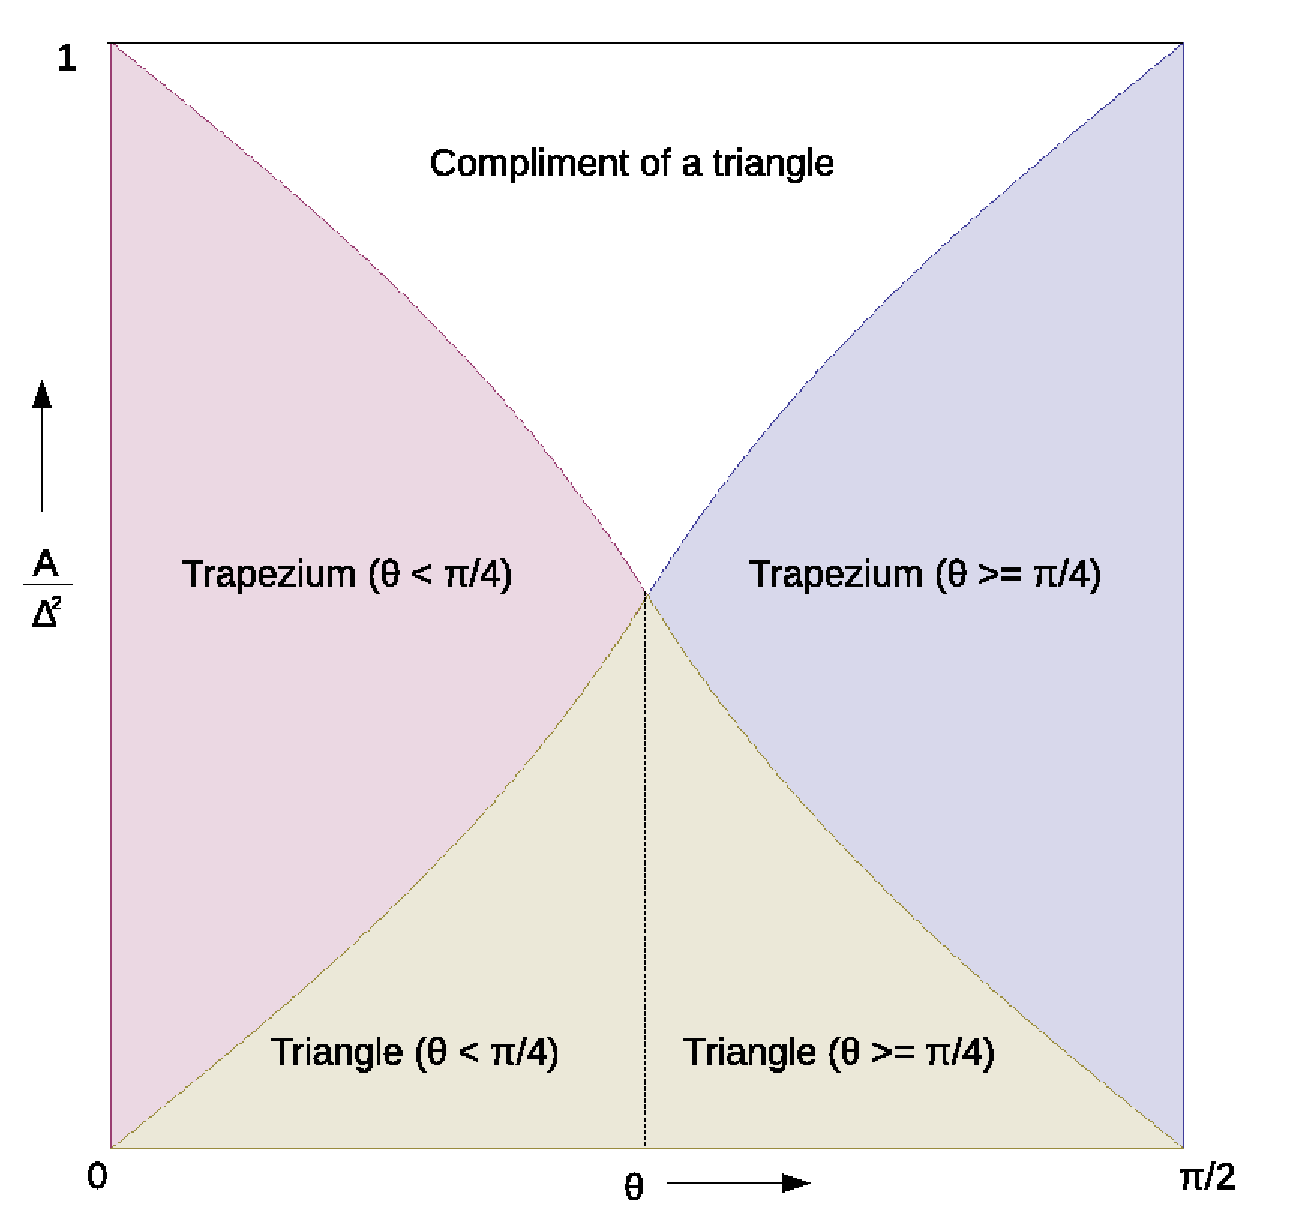
\includegraphics[scale=0.5]{shape_region.eps}
  \caption{Area and angle region}
  \label{Fig:shape_region}
\end{figure}
\underline{Triangle}\\
Area of fluid, $A=\Delta^2F$ 

From Figure \ref{Fig:triangle}, we get,

\begin{figure}%[H] 
\centering
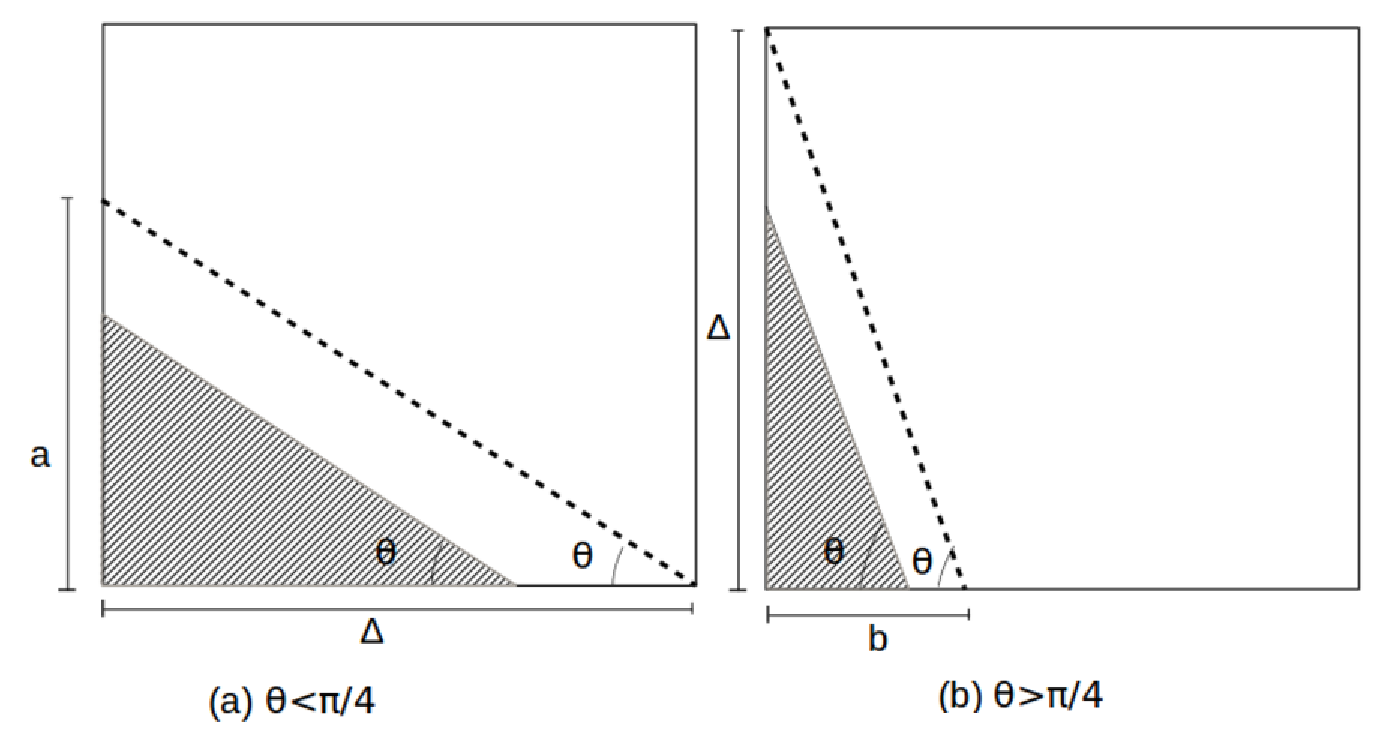
\includegraphics[scale=0.4]{triangle.eps}
\caption{Area of the triangle made by dark fluid in the cell}
\label{Fig:triangle}
\end{figure}

\begin{eqnarray*}
 a&=&\Delta tan\theta \text{\quad $\theta < \frac{\pi}{4}$} \\  
 b&=&\frac{\Delta}{tan\theta} \text{\quad $\theta >= \frac{\pi}{4}$}\\
\end{eqnarray*}

\begin{equation*}
\boxed{\begin{align}
    \frac{A}{\Delta^2} <= \frac{1}{2} tan\theta \qquad \text{for, }\theta < \frac{\pi}{4} \\
    \frac{A}{\Delta^2}<=  \frac{1}{2tan\theta} \qquad \text{for, }\theta > \frac{\pi}{4}   
    \end{align}}
\end{equation*}

\underline{}{For trapezium},\\

\begin{figure}%[H]
\centering
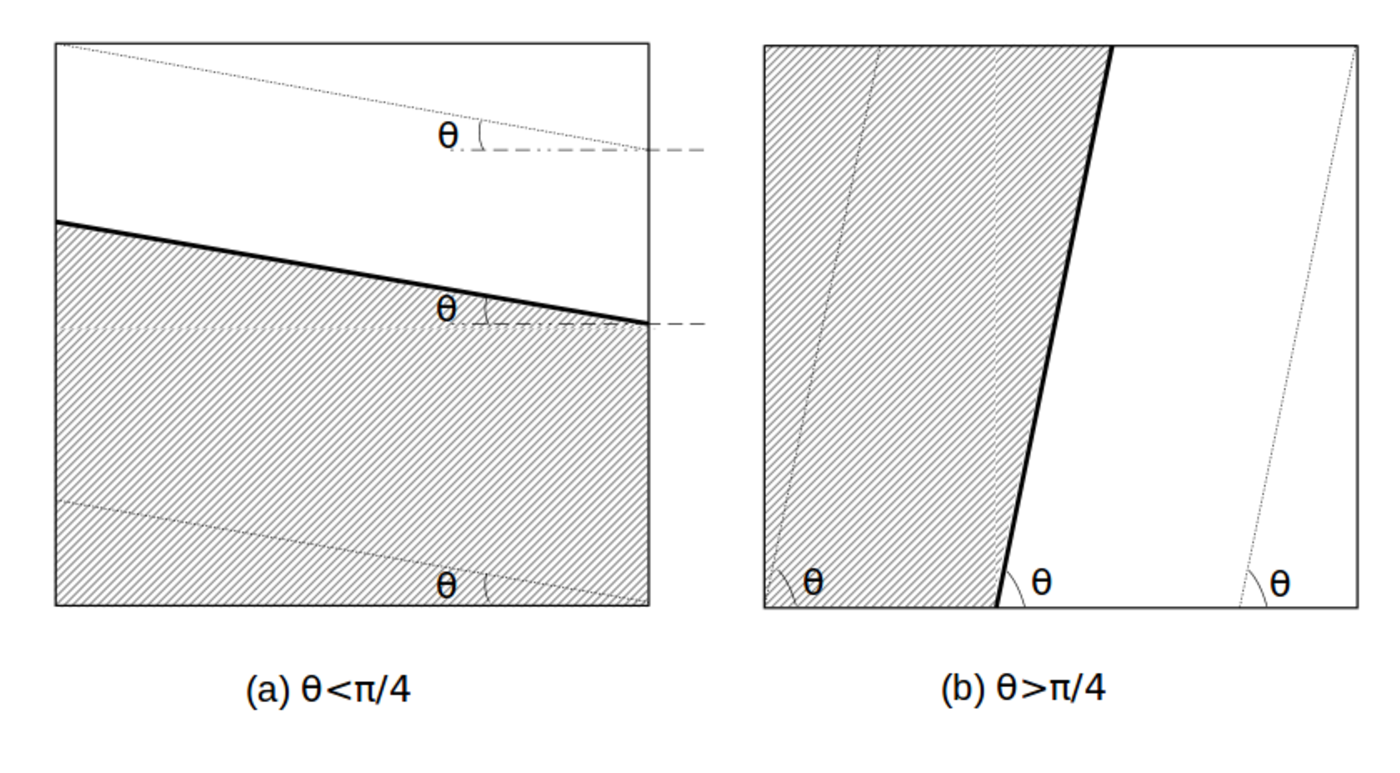
\includegraphics[scale=0.4]{trapezium.eps}
\caption{Area of a trapezium made by the dark fluid in the cell}
\end{figure}

\begin{figure}
 \centering
 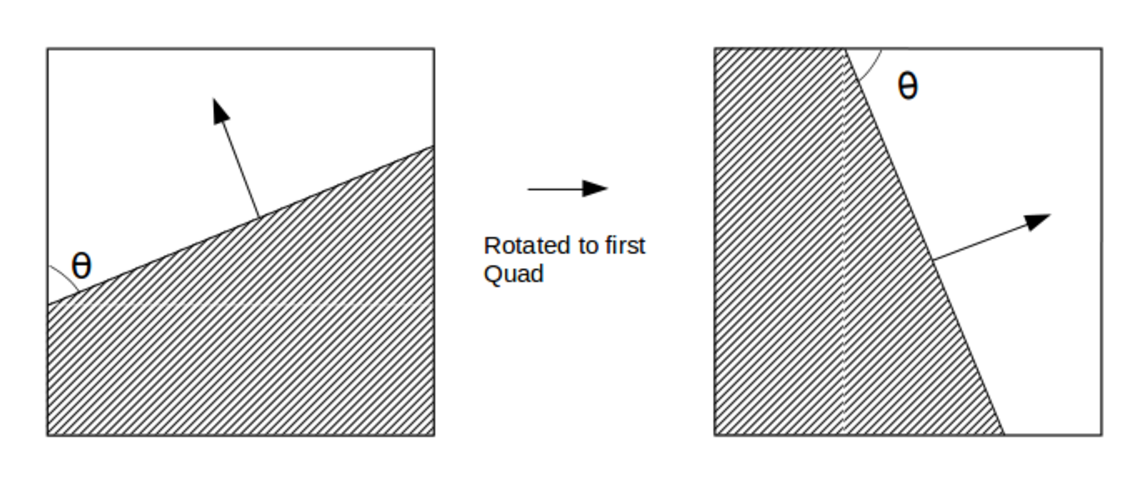
\includegraphics[scale=0.6]{2ndQuad.eps}
 \caption{When the cell is reoriented to make normal lie in first quadrant}
 \label{Fig:reorientation}
\end{figure}

In Figure \ref{Fig:reorientation}, it can be seen that when the cell reoriented to make the normal in first quadrant the $\theta$ becomes the angle with the horizontal axis.
Hence, the same calculations can be applied to this cell for what is done for first quadrant. 

\begin{equation*}
\boxed { \begin{align}
 \frac{1}{2} tan\theta <& \frac{A}{\Delta^2}< \left(1-\frac{1}{2} tan\theta\right)  \qquad \text{for, } \theta < \frac{\pi}{4} \nonumber	\\    
   \frac{1}{2tan\theta} <&   \frac{A}{\Delta^2}< \left(1-\frac{1}{2tan\theta}\right) \qquad \text{for, }  \theta >= \frac{\pi}{4}	
   \end{align}}
\end{equation*}
For all other cases the shape becomes a compliment of a triangle.

\subsubsection{Step VI: Perpendicular distance Calculation }
After reorientation, the perpendicular distance will now be always from the LHS corner of the cell.\\
\underline{Triangle}\\
Note the following formulae for Figure \ref{Fig:trianlge_p}

\begin{eqnarray*}
c=\frac{b}{cos\theta},
\qquad b=\frac{p}{sin\theta},  
\qquad  c=\frac{p}{sin\theta cos\theta},
\qquad   \frac{1}{2}pc=F\Delta^2,
\qquad  \frac{p^2}{sin2\theta}=F\Delta^2 \nonumber
\end{eqnarray*}

\begin{equation*}
\boxed{ \begin{align}
  p=\sqrt{F\Delta^2sin2\theta}
  \end{align} }
\end{equation*}
  
\begin{figure}
\centering
 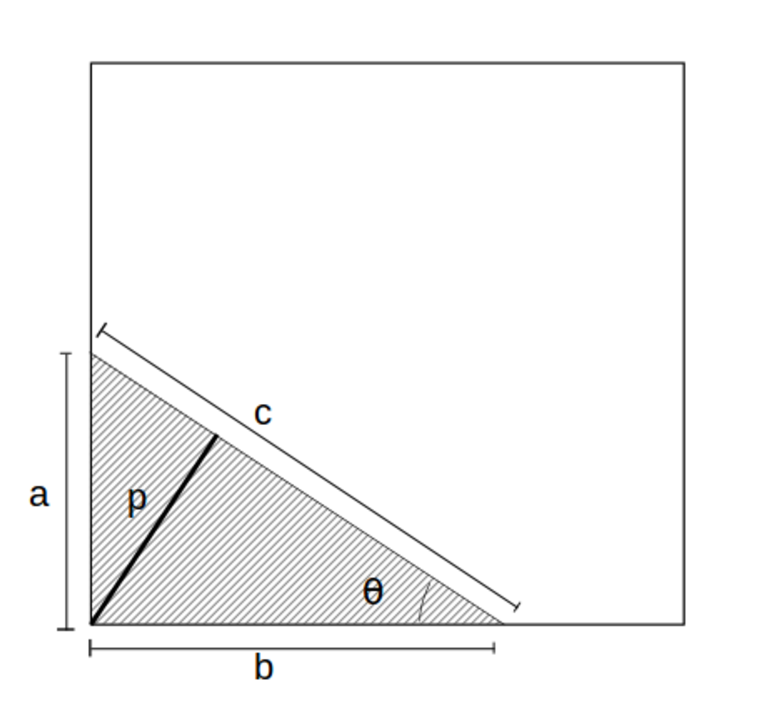
\includegraphics[scale=0.4]{triangle_p.eps}
 \caption{Perpendicular distance in a triangle}
 \label{Fig:trianlge_p}
\end{figure}

\underline{Trapezium}, \\
  \begin{figure}
  \centering
    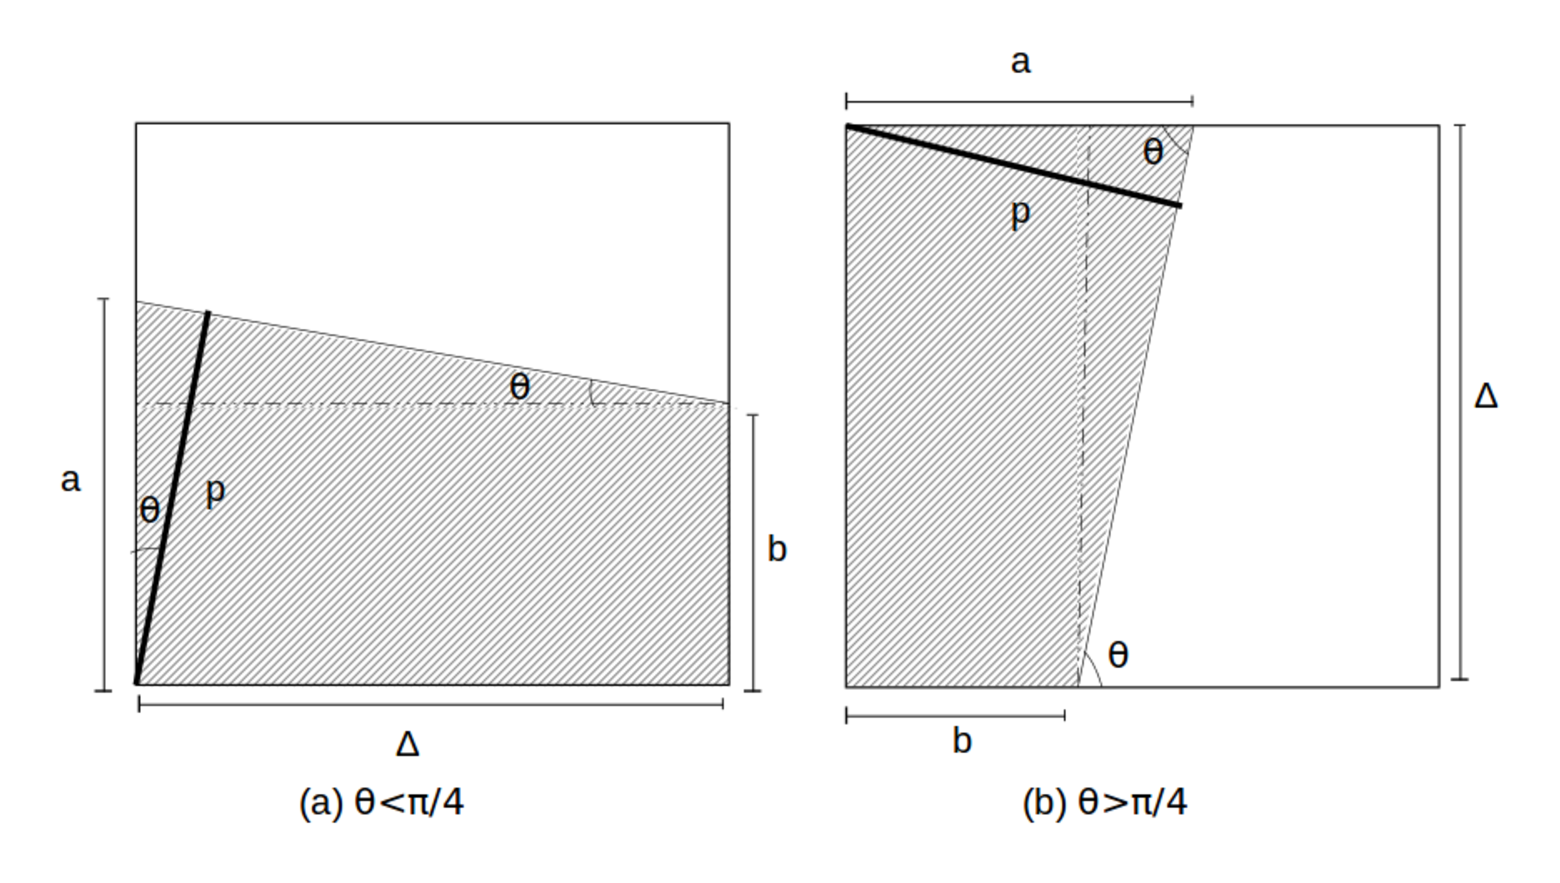
\includegraphics[scale=0.4]{trapezium_p.eps}
    \caption{Perpendicular distance for a trapezium}
    \label{Fig:trapezium_p}
  \end{figure}
  Note the formulae for Figure \ref{Fig:trapezium_p}
  
  \begin{equation*}
  \begin{aligned}  
     \text{For} \quad \theta  < \frac{\pi}{4}, 
    \qquad  \Delta^2 F &=\frac{(a+b)\Delta}{2},
    \qquad a=\frac{p}{cos\theta},
      \qquad tan\theta=\frac{a-b}{\Delta},
      \qquad b=\frac{p}{cos\theta}-\Delta tan\theta, \\
      \\
      \text{or,}\qquad \frac{1}{2}\Delta\left(\frac{2p}{cos\theta}-\Delta tan\theta\right)&=\Delta^2 F,
      \qquad \boxed{p=\Delta Fcos\theta+\frac{1}{2}\Delta sin\theta} \\
      \\
\text{For} \quad \theta  >= \frac{\pi}{4},
\qquad
\Delta^2 F &=\frac{(a+b)\Delta}{2}
\qquad
a=\frac{p}{sin\theta},
\qquad
tan\theta=\frac{\Delta}{a-b},
\qquad
b=\frac{p}{sin\theta}-\frac{\Delta}{tan\theta},\\
\\
\text{or,}\qquad 0.5\Delta\left(\frac{2p}{sin\theta}-\frac{\Delta}{tan\theta}\right)&=\Delta^2 F,
\qquad
\boxed{p=\Delta Fsin\theta+\frac{1}{2}\Delta cos\theta}
\end{aligned}
  \end{equation*}
  
\underline{For compliment of triangle},
\begin{figure}[H]
\centering
 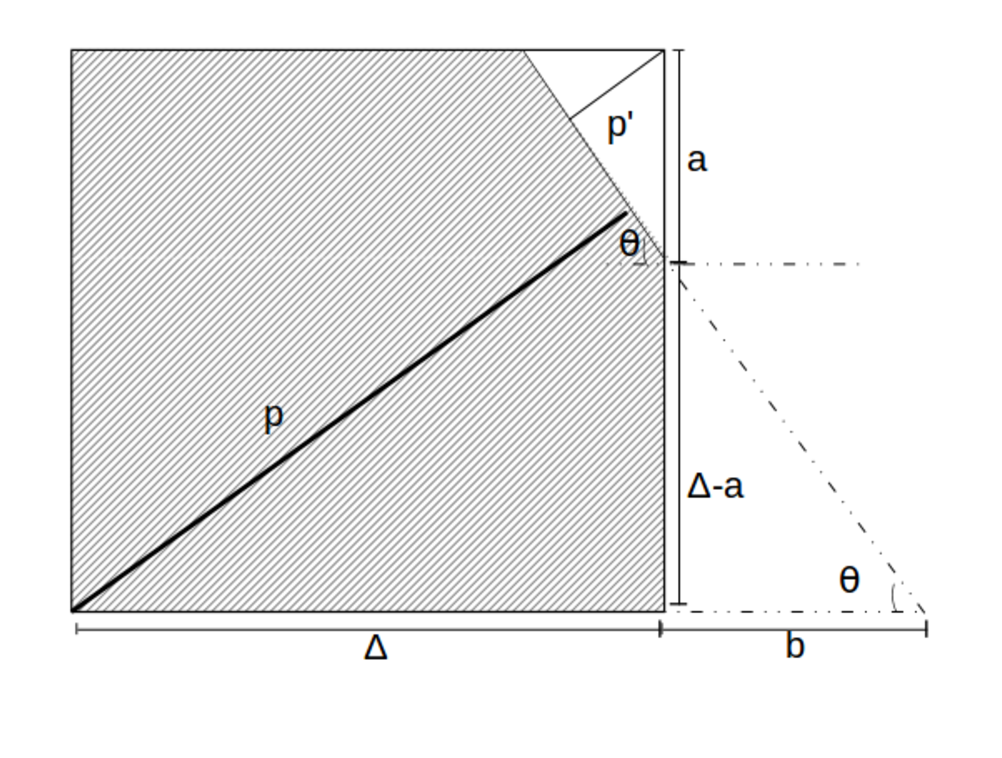
\includegraphics[scale=0.3]{compliment_p.eps}
 \caption{Perpendicular distance for compliment of the triangle}
\end{figure}

\begin{equation*}
\begin{align}
 p'&=&\sqrt{F\Delta^2sin2\theta},
\qquad a=\frac{p'}{cos\theta},\\
\\
\text{or,}\qquad b&=&\frac{\Delta-a}{tan\theta},
\qquad \boxed{p=\Delta(sin\theta+cos\theta)-p'}
\end{align}
\end{equation*}

\subsubsection{Step VII : Line Extrapolation}
After, reorientation of the line to the first quadrant. A line can be constructed with the $\theta$ and perpendicular distance using normal form, (See Figure \ref{Fig:normal})
\begin{figure}
 \centering
 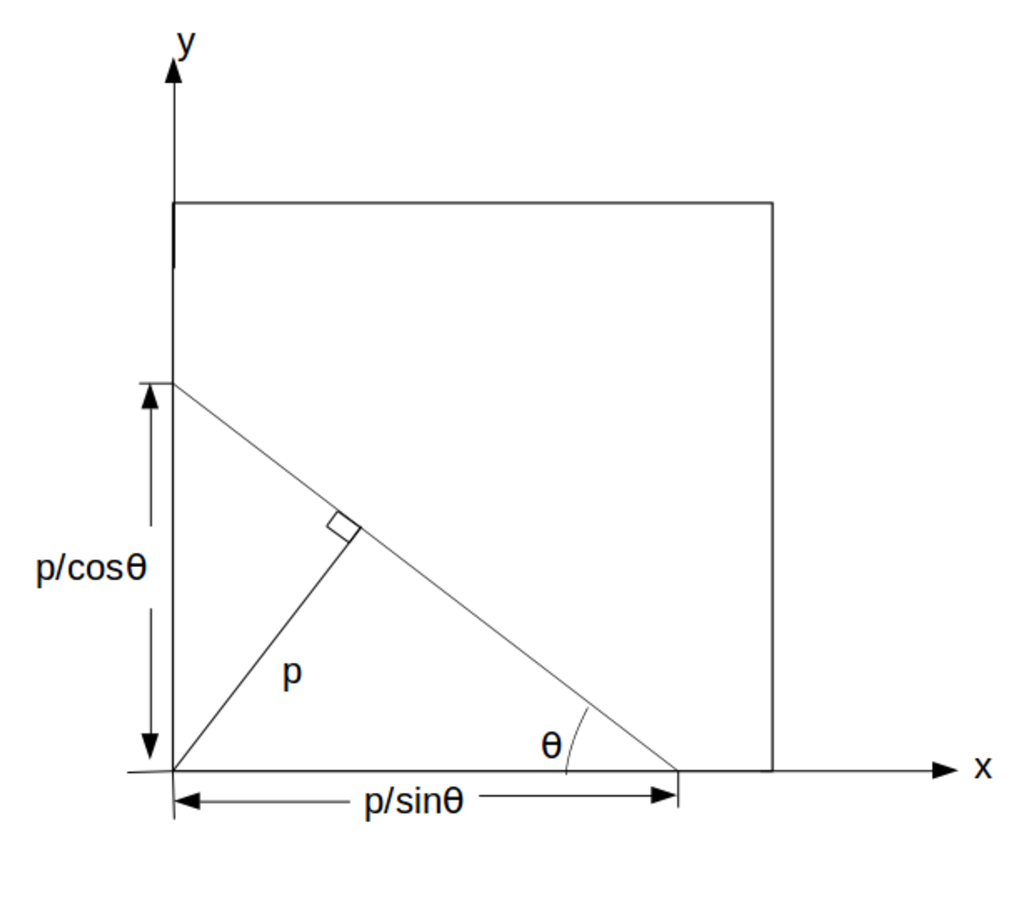
\includegraphics[scale=0.4]{normal_form.eps}
 \caption{Normal form of a line in the cell}
 \label{Fig:normal}
\end{figure}
\begin{equation}
 x\sin\theta+y\cos\theta = p
\end{equation}

Refer to Figure \ref{Fig:extrapolation} for extrapolation,

\begin{figure}%[H]
 \centering
 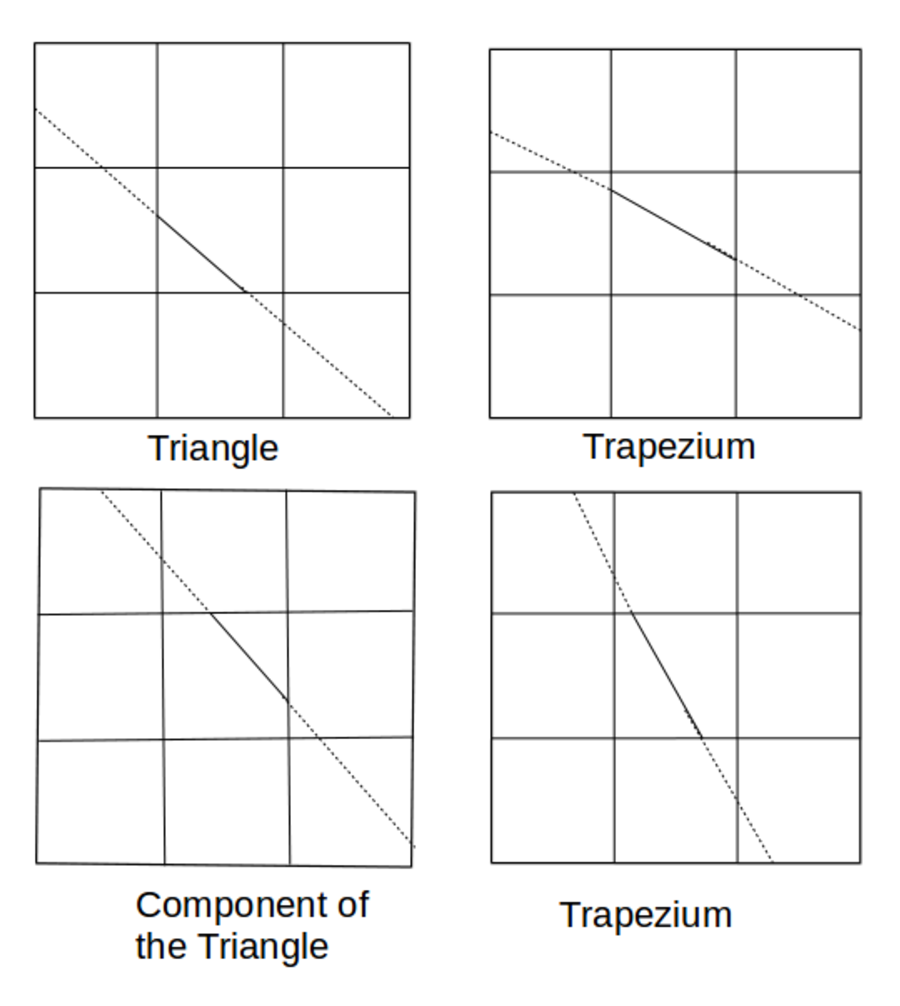
\includegraphics[scale=0.4]{extrapolate.eps}
 \caption{Extrapolation of the line in 3 X 3 cell}
 \label{Fig:extrapolation}
\end{figure}

After extrapolation the new volume fraction is calculated under each cell below the line, which is then used to calculate the norm.
\subsubsection{Step VIII: Norm Calculation}
Let the new volume fraction calculated be $\widetilde F_{r,c}$. Now the norm which is here the difference of original volume fraction and new 
volume fraction calculated after the extrapolation are squared and then summed over 3 X 3 stencil. Also, called as $L^2$ norm, \\
\begin{equation*}
 \boxed{L^2(\theta) =  \sum_{k,l=-1}^{1}(\widetilde F_{r+k,c+l}-F_{r+k,c+l})^2}
\end{equation*}

\subsubsection{Step IX : Norm Minimization}
After calculating norm the initial guess of slope and $\theta$ is changed with small step size but it should not be confused with rotation of interface or normal.
All the steps are repeated to after modifying theta and norm is again calculated. This process repeats when a minima of norm reached. And the final values of $\theta$,
shape, and quadrant are assigned to the cell.

\subsection{Advection}
The Equation \ref{Eq:advection_vof} is also solved using geometrical technique by calculating fluxes across the cells and then updating the F-field in each time step. Direct finite differencing
of this equation will lose the discontinuous property of F-field and cause smearing of interface as shown in Figure \ref{Fig:smearing}\\
% 
\underline{Flux Calculation}\\
% The flux is calculated through the wall of the cells in X an Y directions.
% for first quadrant all cases are discussed below, for all other quadrants reorientation of normal works,
% For X-Flux when velocity in x-direction, u is positive then only the right wall of the left cell will affect the flux (See Figure 11)
The flux of fluid through the walls is calculated using a graphical technique. A typical cell is shown in Figure \ref{Fig:triangle_t} and the through its right wall is calculated .
Various possibilities arise and these are discussed below.
\subsubsection{\underline{Triangle}}
For a triangle there are two cases:-\\
if $(\Delta-udt)>x_0$, Nothing will leave from the right wall \\
if $(\Delta-udt)<x_0$, A triangle leaves. \\
here $x_0$ is the value of x at $y=0$.
\begin{figure}%[H]
 \centering
 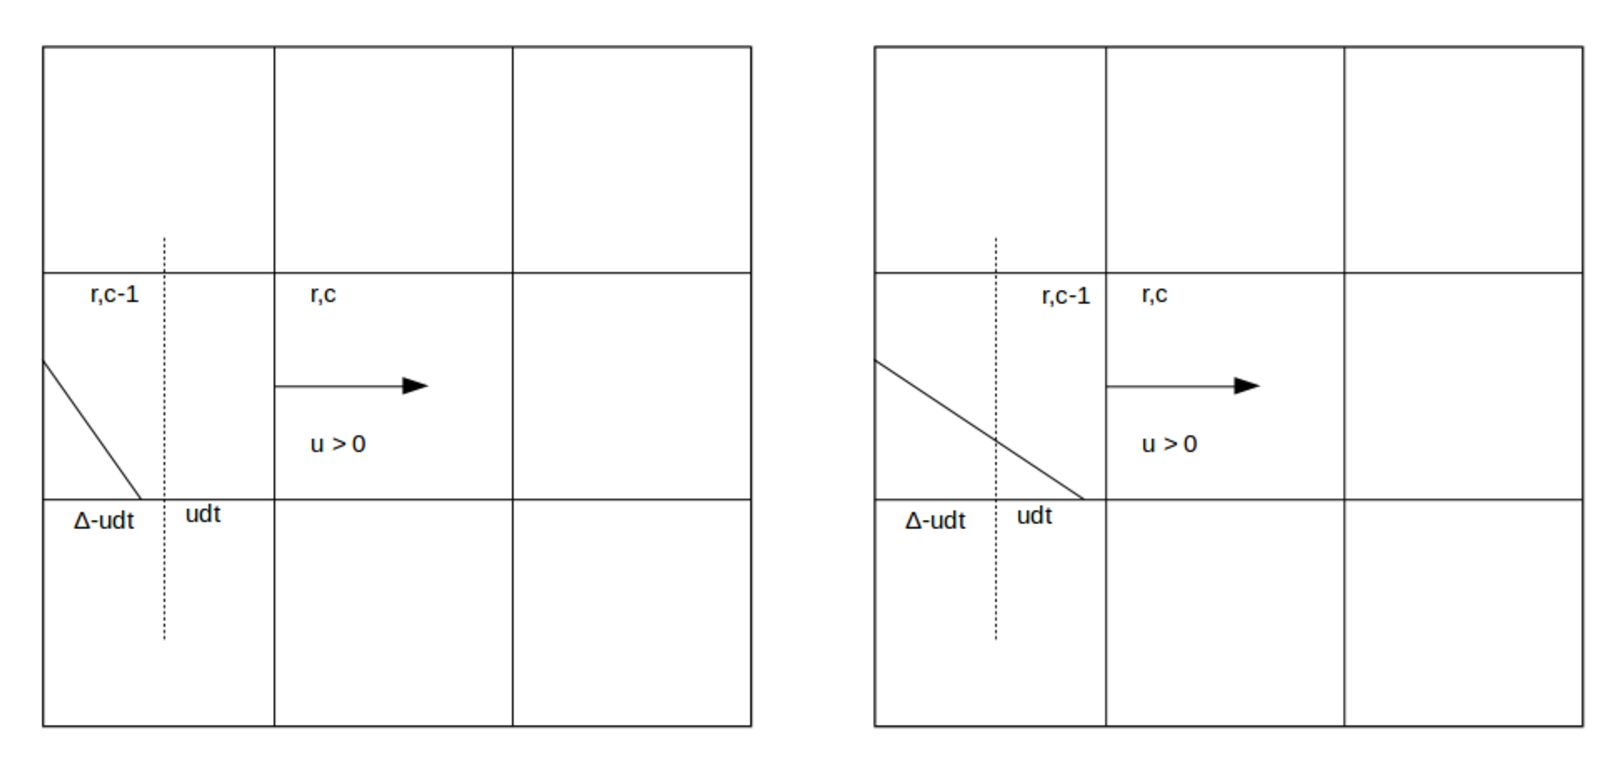
\includegraphics[scale=0.4]{ad_triangle.eps}
 \caption{Cases for a triangle in flux calculation}
 \label{Fig:triangle_t}
\end{figure}
The area of this triangle is given by,
\begin{equation*}
 \boxed{Flux = \frac{1}{2}(x_0 - \Delta + udt)^2 \tan\theta}
\end{equation*}

\subsubsection{\underline{Trapezium}}
Two types of trapezium can be in the first quadrant, $\theta<\frac{\pi}{4}$, and $\theta>\frac{\pi}{4}$, \\
(See Figure \ref{Fig:trapezium} and \ref{Fig:trapezium_cases}) \\
\begin{figure}%[H]
\centering
 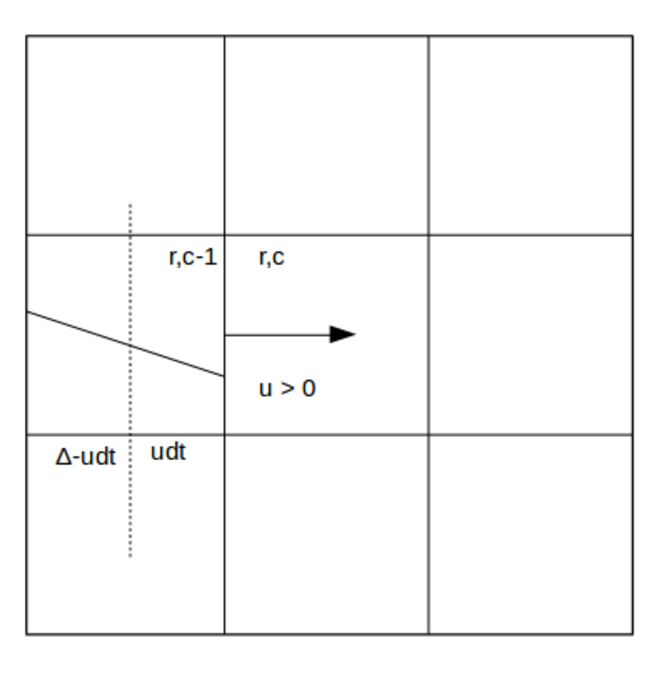
\includegraphics[scale=0.4]{ad_trapezium.eps}
 \caption{Flux calculation for trapezium for $\theta<\frac{\pi}{4}$}
 \label{Fig:trapezium}
\end{figure}

\begin{figure}%[H]
 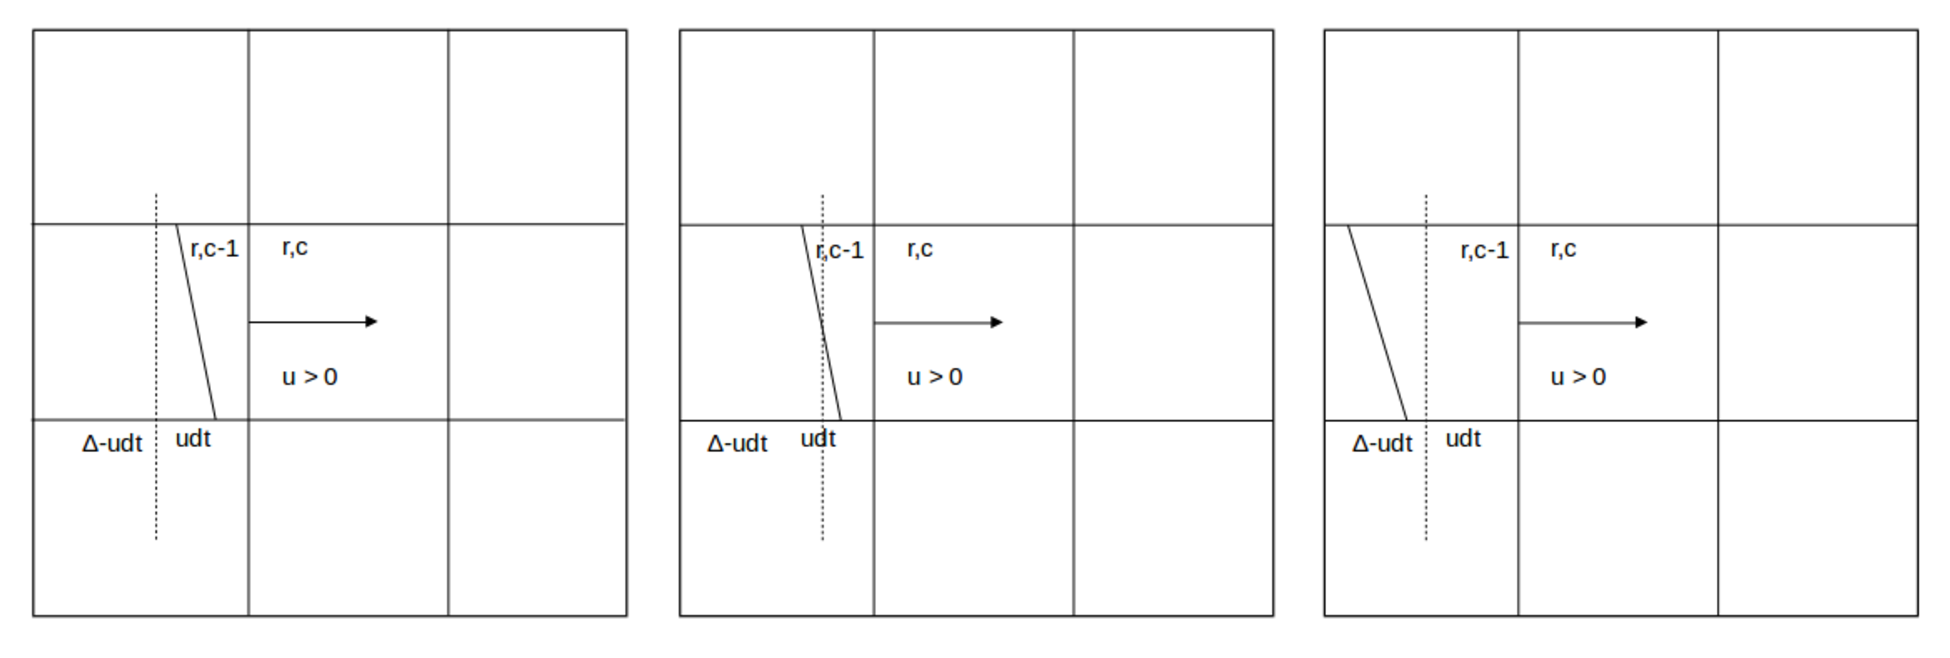
\includegraphics[scale=0.4]{ad_trap_pi4.eps}
 \caption[Different cases for flux calculation for trapezium]{(a)$(\Delta-udt)<x_{del}$, (b)$x_{del}<=(\Delta-udt)<x_0$, (c)$(\Delta-udt)>=x_0$}
 \label{Fig:trapezium_cases}
\end{figure}

For $\theta<\frac{\pi}{4}$, the only possibility is that a trapezium leaves and its area is given by,
\begin{eqnarray*}
 Flux = \frac{1}{2}( y_0 - ((\Delta - udt) \tan\theta) + y_{del} ) udt \\
\end{eqnarray*}

\begin{equation*}
 \begin{align}
 &\text{For } \theta>\frac{\pi}{4}, \\
 \text{For } &(\Delta-udt)<x_{del},  \text{ a trapezium leaves the cell and the Flux is given by,} \\
&\boxed{ Flux = \frac{\Delta}{2}(x_{del} - (2(\Delta - udt)) + x_0) }\\
 \text{For }  &x_{del}<=(\Delta-udt)<x_0,  \text{ a triangle leaves the cell and the flux is given by,} \\
&\boxed{Flux =\frac{1}{2\tan\theta} (y_0 - (\Delta - udt)\tan\theta))^2} \\
\text{For } & ((\Delta-udt))>=x_0,  \text{nothing leaves from the cell.} \\
&\boxed{Flux =0}
\end{align}
\end{equation*}

\subsubsection{\underline{Compliment of a triangle}}
For compliment of a triangle two cases arise, (See Figure \ref{Fig:compliment_triangle})
\begin{figure}%[H]
 \centering
 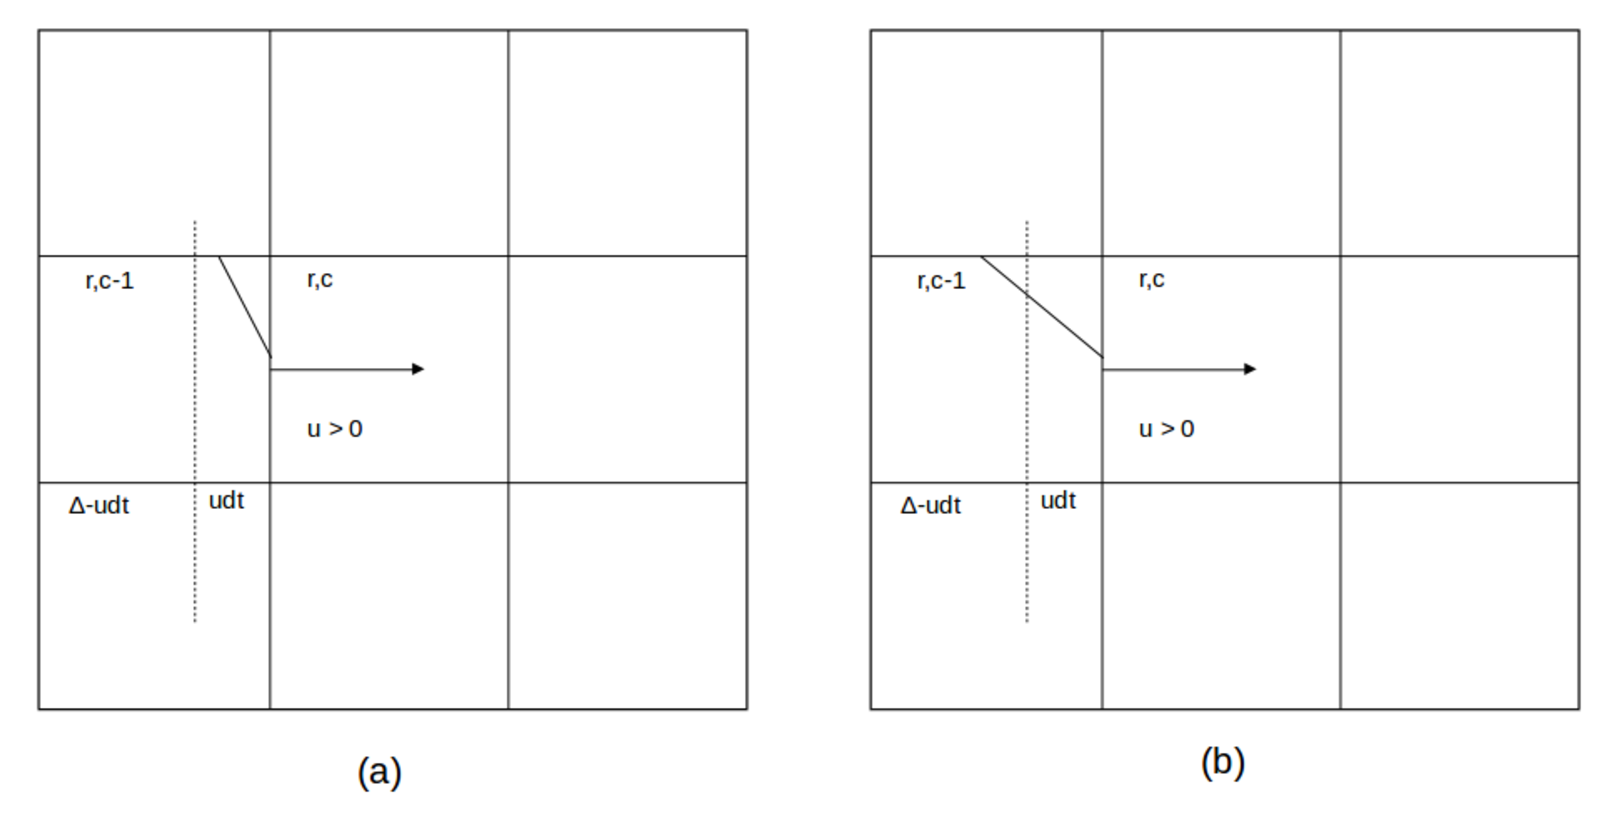
\includegraphics[scale=0.4]{ad_comp.eps}
 \caption[Different cases for flux calculation for compliment of a triangle]{(a)$(\Delta-udt) < x_{del}$, (b)$(\Delta-udt) >= x_{del}$}
 \label{Fig:compliment_triangle}
\end{figure}
\begin{equation*}
\begin{aligned}
\text{if, } \Delta -udt &< x_{del}, \text{ A 5-Sided figure leaves,  and Flux is given by,} \\
&\boxed{Flux = \Delta(x_{del} - \Delta + udt)) + \frac{1}{2}((\Delta + y_{del})(\Delta - x_{del}))} \text{ (sum of rectangle and trapezium)} \\
\text{if, } \Delta -udt &>= x_{del},  \text{ A trapezium leaves, and Flux is given by,} \\
&\boxed{Flux =  \frac{udt}{2}( y_{del} + y_0 - (\Delta - udt)\tan\theta)}
\end{aligned}
\end{equation*}

\subsection{Volume Fraction Calculation}
The fluxes calculated in the previous section are used to update the volume fractions in the cells for the next time step. For this we use \textit{Direction Split Young's method} (DSY).
\cite{Youngs1982}. In this method the order of directions is interchanged after each time step in order to avoid systematic errors. To achieve mass conservation, for this the 
basic condition is velocity divergence. In this method, the mass cannot be conserved until all directions are taken into consideration. Hence the values of volume fraction larger than unity
and less than zero may arise after first sweep which violates the restriction, $0\leqslant F\geqslant=1$ for the next sweep. This difficulty can be solved by introducing effective 
volume of the cells (\cite{Rudman1997}). But this induces risks of small under- or overshoots. Undershoot occurs when the all the volume fraction has to be fluxed out from the cell 
but it does not and cell cannot be emptied, overshoot occurs when the cell in fluxed with the volume fraction to get filled but it does not. Both occurs because of use of effective volume
in calculation of fluxes through wall. This can be resolved by using flux correction in the second sweep \cite{Lorstad2004}. The following algorithm is used to calculate the volume 
fractions for the 2D flow. \\
Effective volume(non-dimensional, characteristic area $\Delta^2$) for the $I^{st}$ sweep,
\begin{equation*}
 \delta V^I_{r,c} = 1 - \Delta t \frac{V_{out}-V_{in}}{\Delta} 
\end{equation*}
where, $\delta V^I_{r,c}$ is the effective volume after $I^{st}$ sweep. \\
Net Flux out $\Delta J_{out}$, (non-dimensional) in or out in a cell is given by,
\begin{equation*}
 \Delta J_{out} = \frac{(J_{out}-J_{in})}{\Delta^2} 
\end{equation*}

From which Volume Fraction after $I^{st}$ of the cell is given by,
\begin{equation*}
\boxed{F_{r,c}^I =  \frac{F^0 - \Delta J_{out}}{\delta V^1_{r,c}}}
\end{equation*}
where, $F^0$ and $F^I$ are the volume fractions before $I^{st}$ sweep and after $I^{st}$ sweep respectively.

For $II^{nd}$ sweep, 
\begin{equation*}
 \begin{align}
U^*_{out}  &= \frac{\Delta t}{\Delta}u_{out} \\
 \zeta &=
\begin{cases}
 \zeta_1 = \frac{J_{out}}{U^*_{out}} & \text{if} |\zeta_1-\frac{1}{2}| \geqslant  |\zeta_2-\frac{1}{2}| \\
\zeta_2 = \frac{F_{r,c}-J_{out}}{1-U^*_{out}} & \text{if} |\zeta_1-\frac{1}{2}| <  |\zeta_2-\frac{1}{2}| 
\end{cases} \\
\text{Corrected volume is given by,} \\
\delta V^{corr} &= F_{r,c} + (1-\delta V_{r,c}^I)\zeta \\
\text{Corrected outgoing flux is given by,} \\
J_{out}^{corr} &=  \delta V_{r,c}^I (J_{out}-U^*_{out}) + \delta V^{corr} U^*_{out} \\
\text{Corrected Total flux out from the cell is given by }\\
 \Delta J_{out}^{corr} &= J_{out}^{corr} - J_{in} \\
 \end{align}
 \end{equation*}
 \begin{equation*}
 \begin{align}
 \text{Final flux after last sweep is given by,}\\
 \boxed{F_{r,c}^{II} = F_{r,c}^{I} \delta V_{r,c}^I -  \Delta J_{out}^{corr}}
 \end{align}
\end{equation*}




\begin{figure}
 \subfloat[A circular interface\label{fig:1}]{%
      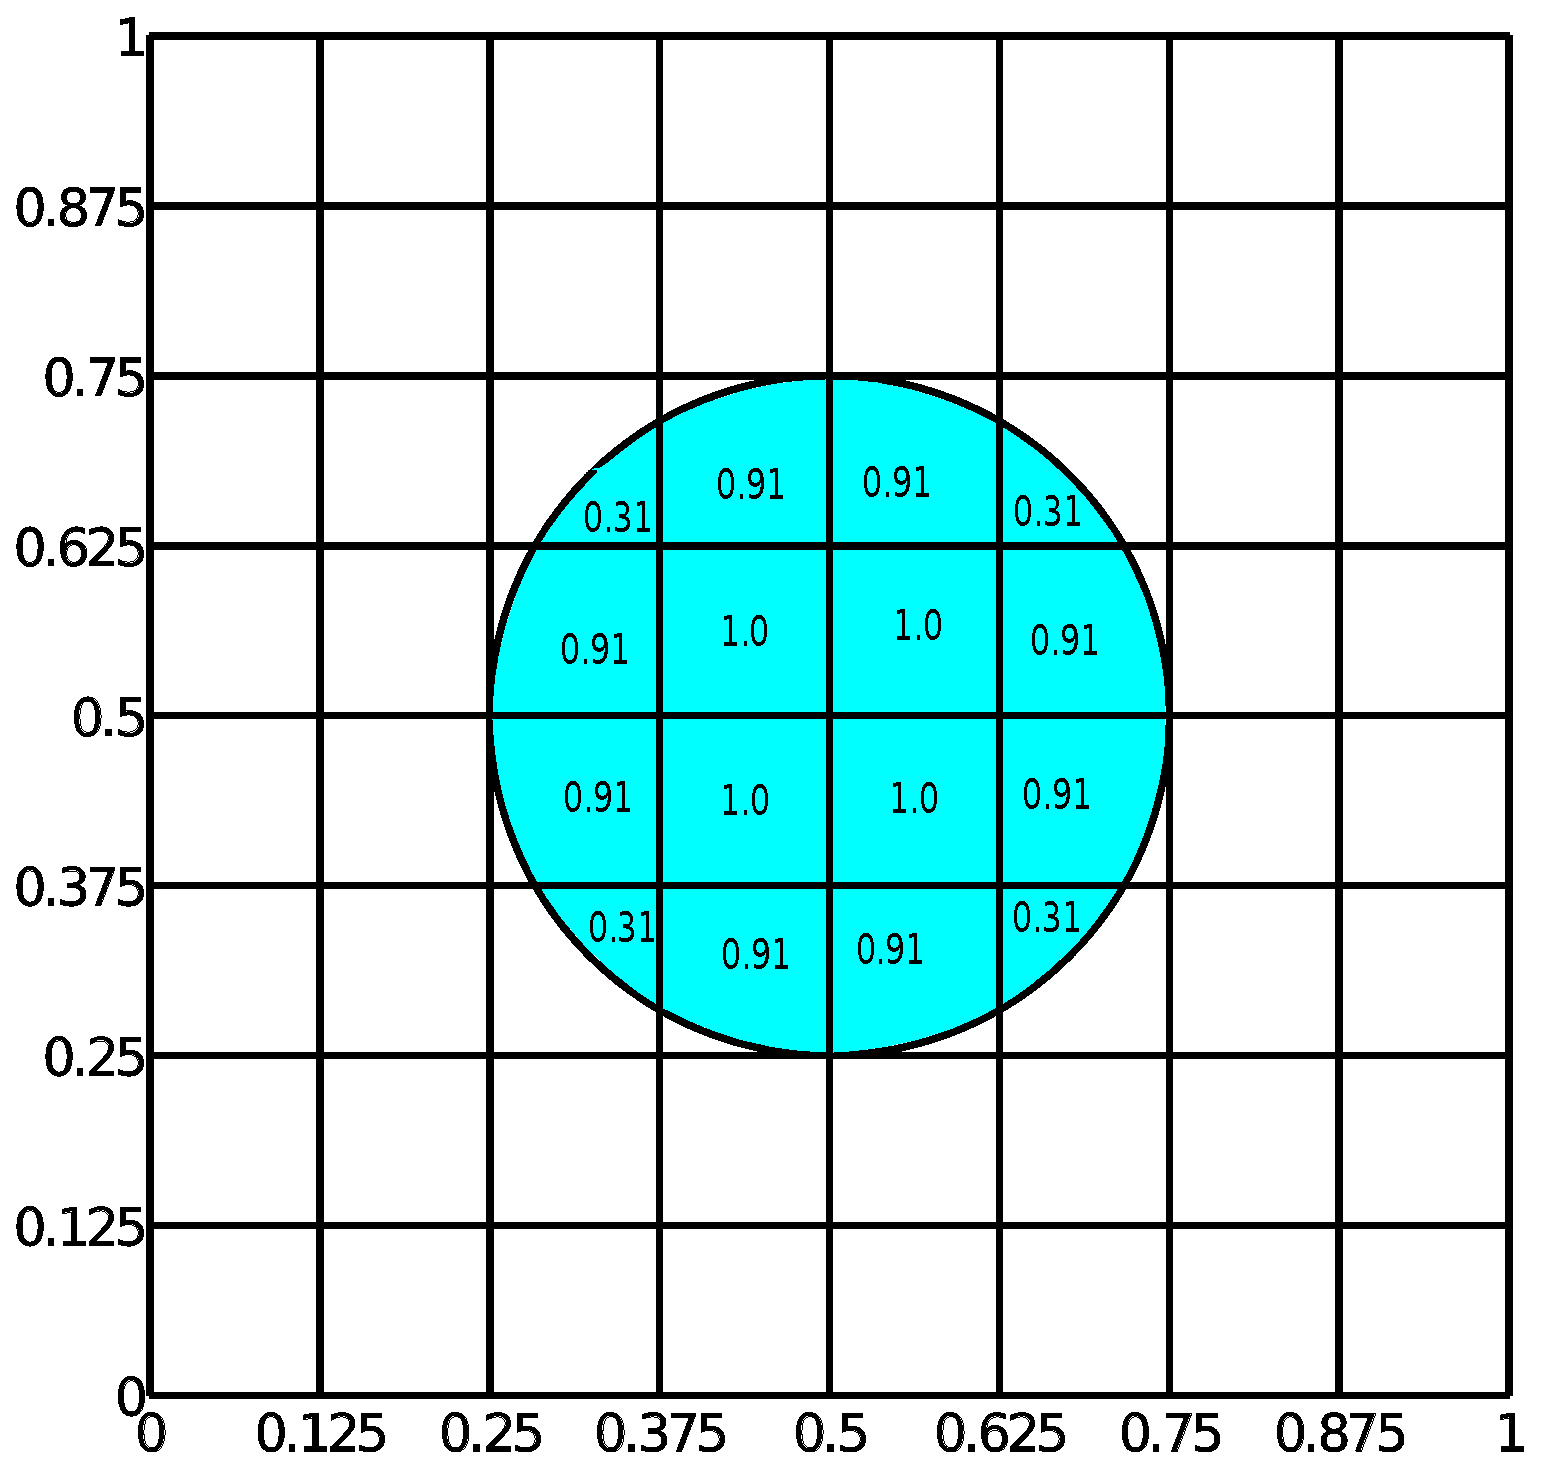
\includegraphics[width=0.5\textwidth]{circle_original_new.eps}
      }
  \subfloat[Reconstruction by LVIRA\label{fig:2}]{%
      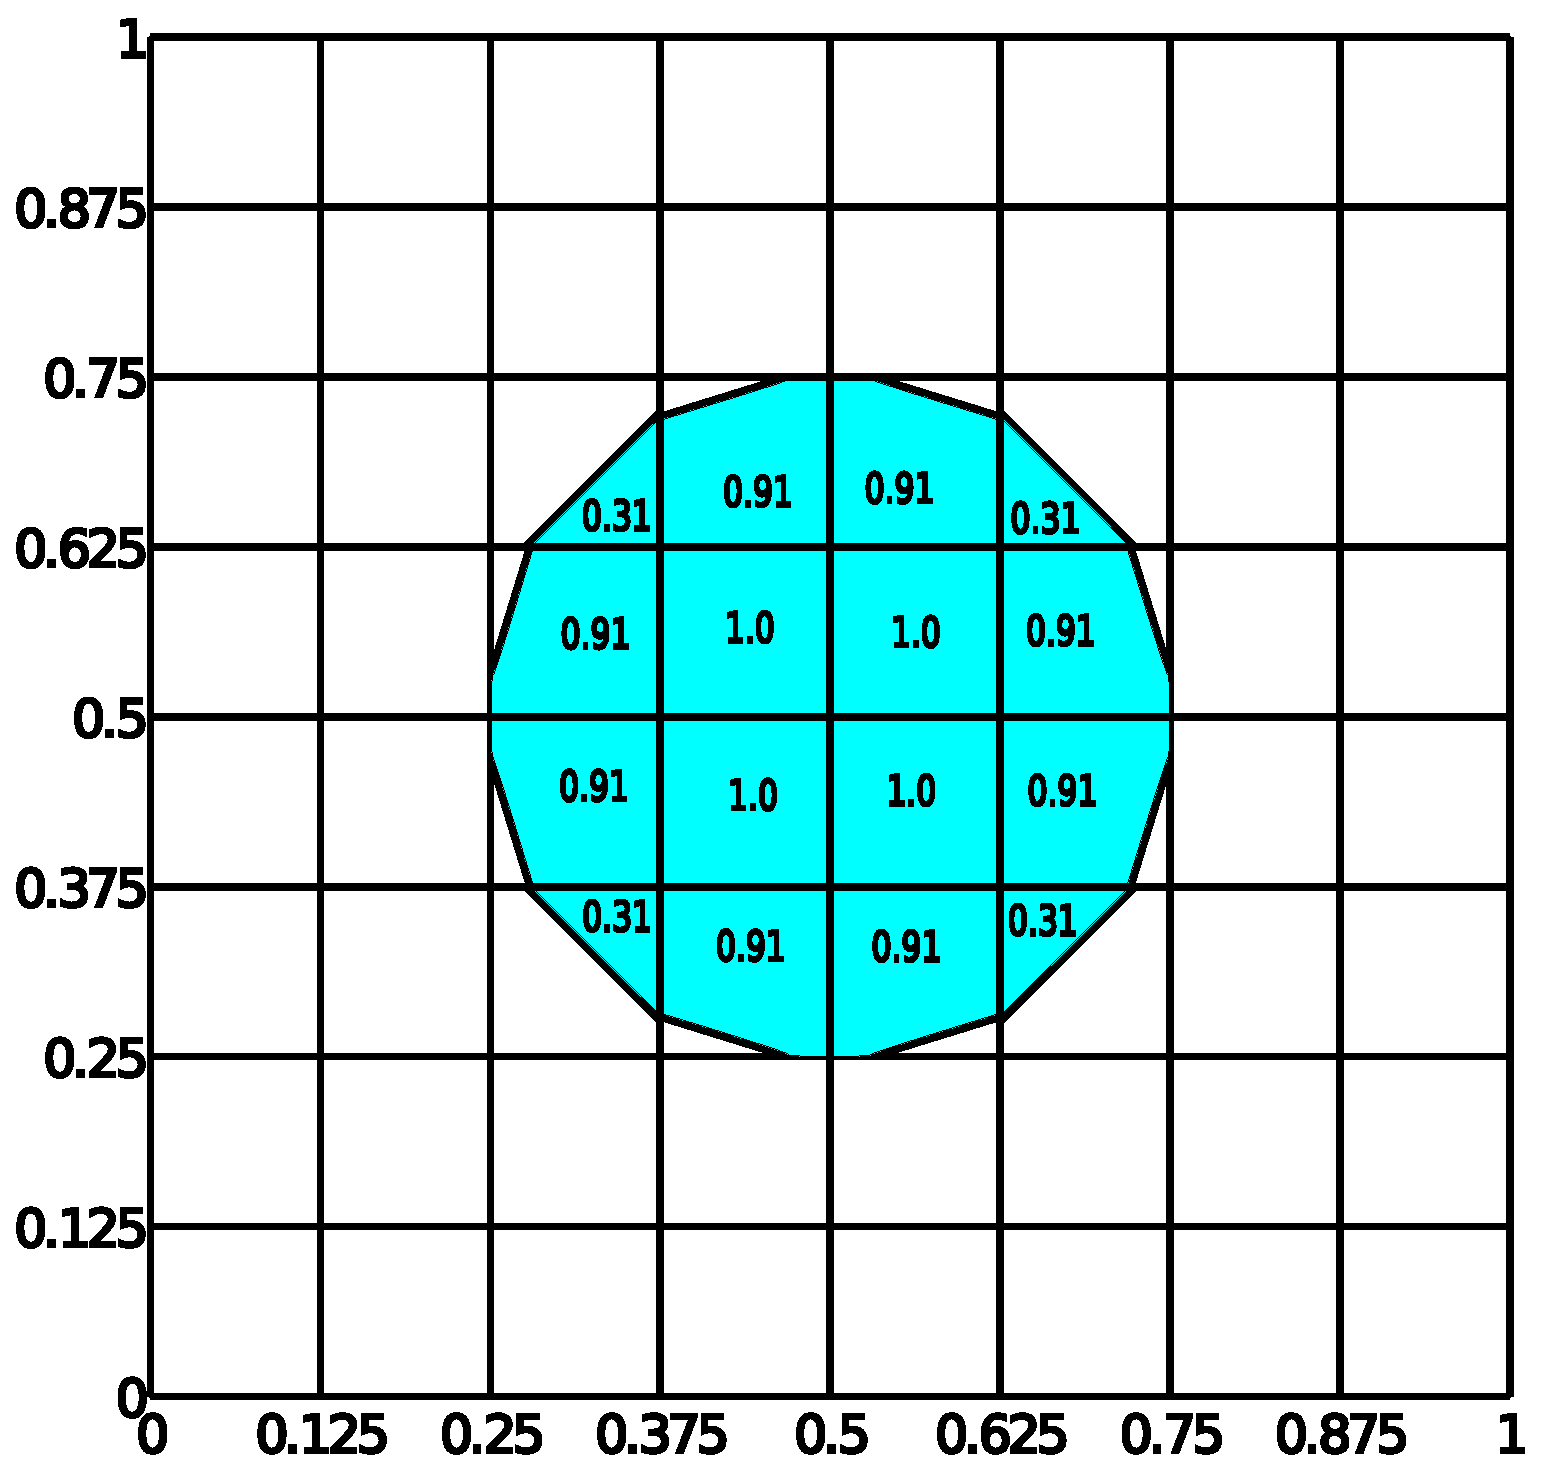
\includegraphics[width=0.5\textwidth]{circle_Recon_LVIRA.eps}
      }
 \caption{Reconstruction of a circular interface by LVIRA}
\end{figure}

\begin{figure}
 \subfloat[Flux calculation in x-direction\label{fig:3}]{%
      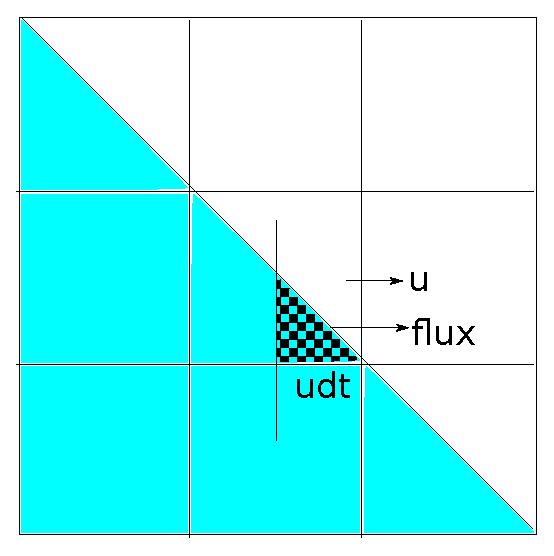
\includegraphics[width=0.5\textwidth]{u_ad.eps}
      }
  \subfloat[Flux calculation in x-direction\label{fig:4}]{%
      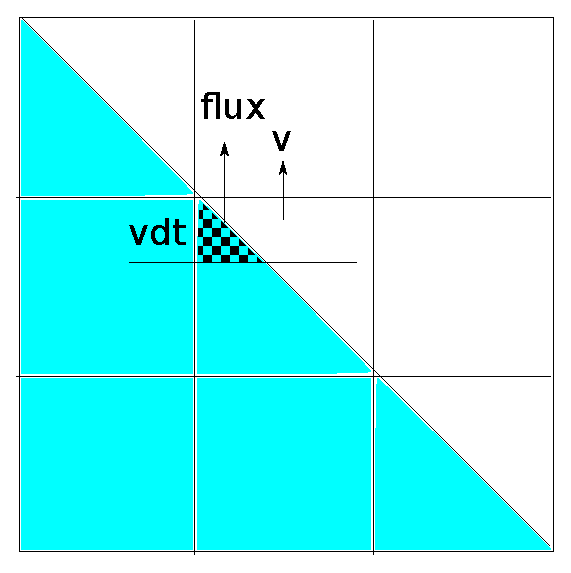
\includegraphics[width=0.5\textwidth]{v_ad.eps}
      }
 \caption{Advection of the interface by Youngs operator split algorithm}
\end{figure}

\section{Verification}
There are standard test cases are available in the literature: \cite{Zalesak1979}, \cite{Puckett1997}, \cite{Anton2001}, \cite{Gerlach2006} etc.
These involve advecting the interface with a fixed underlying velocity field of varying degree of complexity.
Volume of Fluid method is validated by choosing three test cases from \cite{Rudman1997}, 

\begin{enumerate}
 \item \textbf{Circle in translational flow} \\
 In this test the velocity field has zero velocity gradient and it is the simplest of all the tests.
 \item \textbf{Solid body rotation of slotted circle} \\
 The test has rate of strain tensor zero and gradient of velocity only has the vorticity component with constant angular velocity at every point in space.
 \item \textbf{Circle in shear flow} \\
Vorticity tensor in this test is zero and there is only the rate of strain tensor.
\end{enumerate}

\subsection{Advection of circle in translational flow}
The algorithm is tested for the simplest case of unidirectional velocity field. Two concentric circles are used as the initial 
condition for translational test, with center at (0.75,1) and diameter of inner and outer circle is 0.4 and 0.8 respectively (Figure \ref{Fig:translational_test}).
The volume fraction scalar field is advected by two velocity fields u=1,v=0 and u=2,v=1. The refinement of the domain which is [0,4] x [0,4] is 200 x 200. The time
step is 0.005 units and advection proceeds for 500 and 504 steps for case 1 and case 2 respectively.

\begin{figure}%[H]
 \centering
 \subfloat[Initial Condition for translational test]{%
      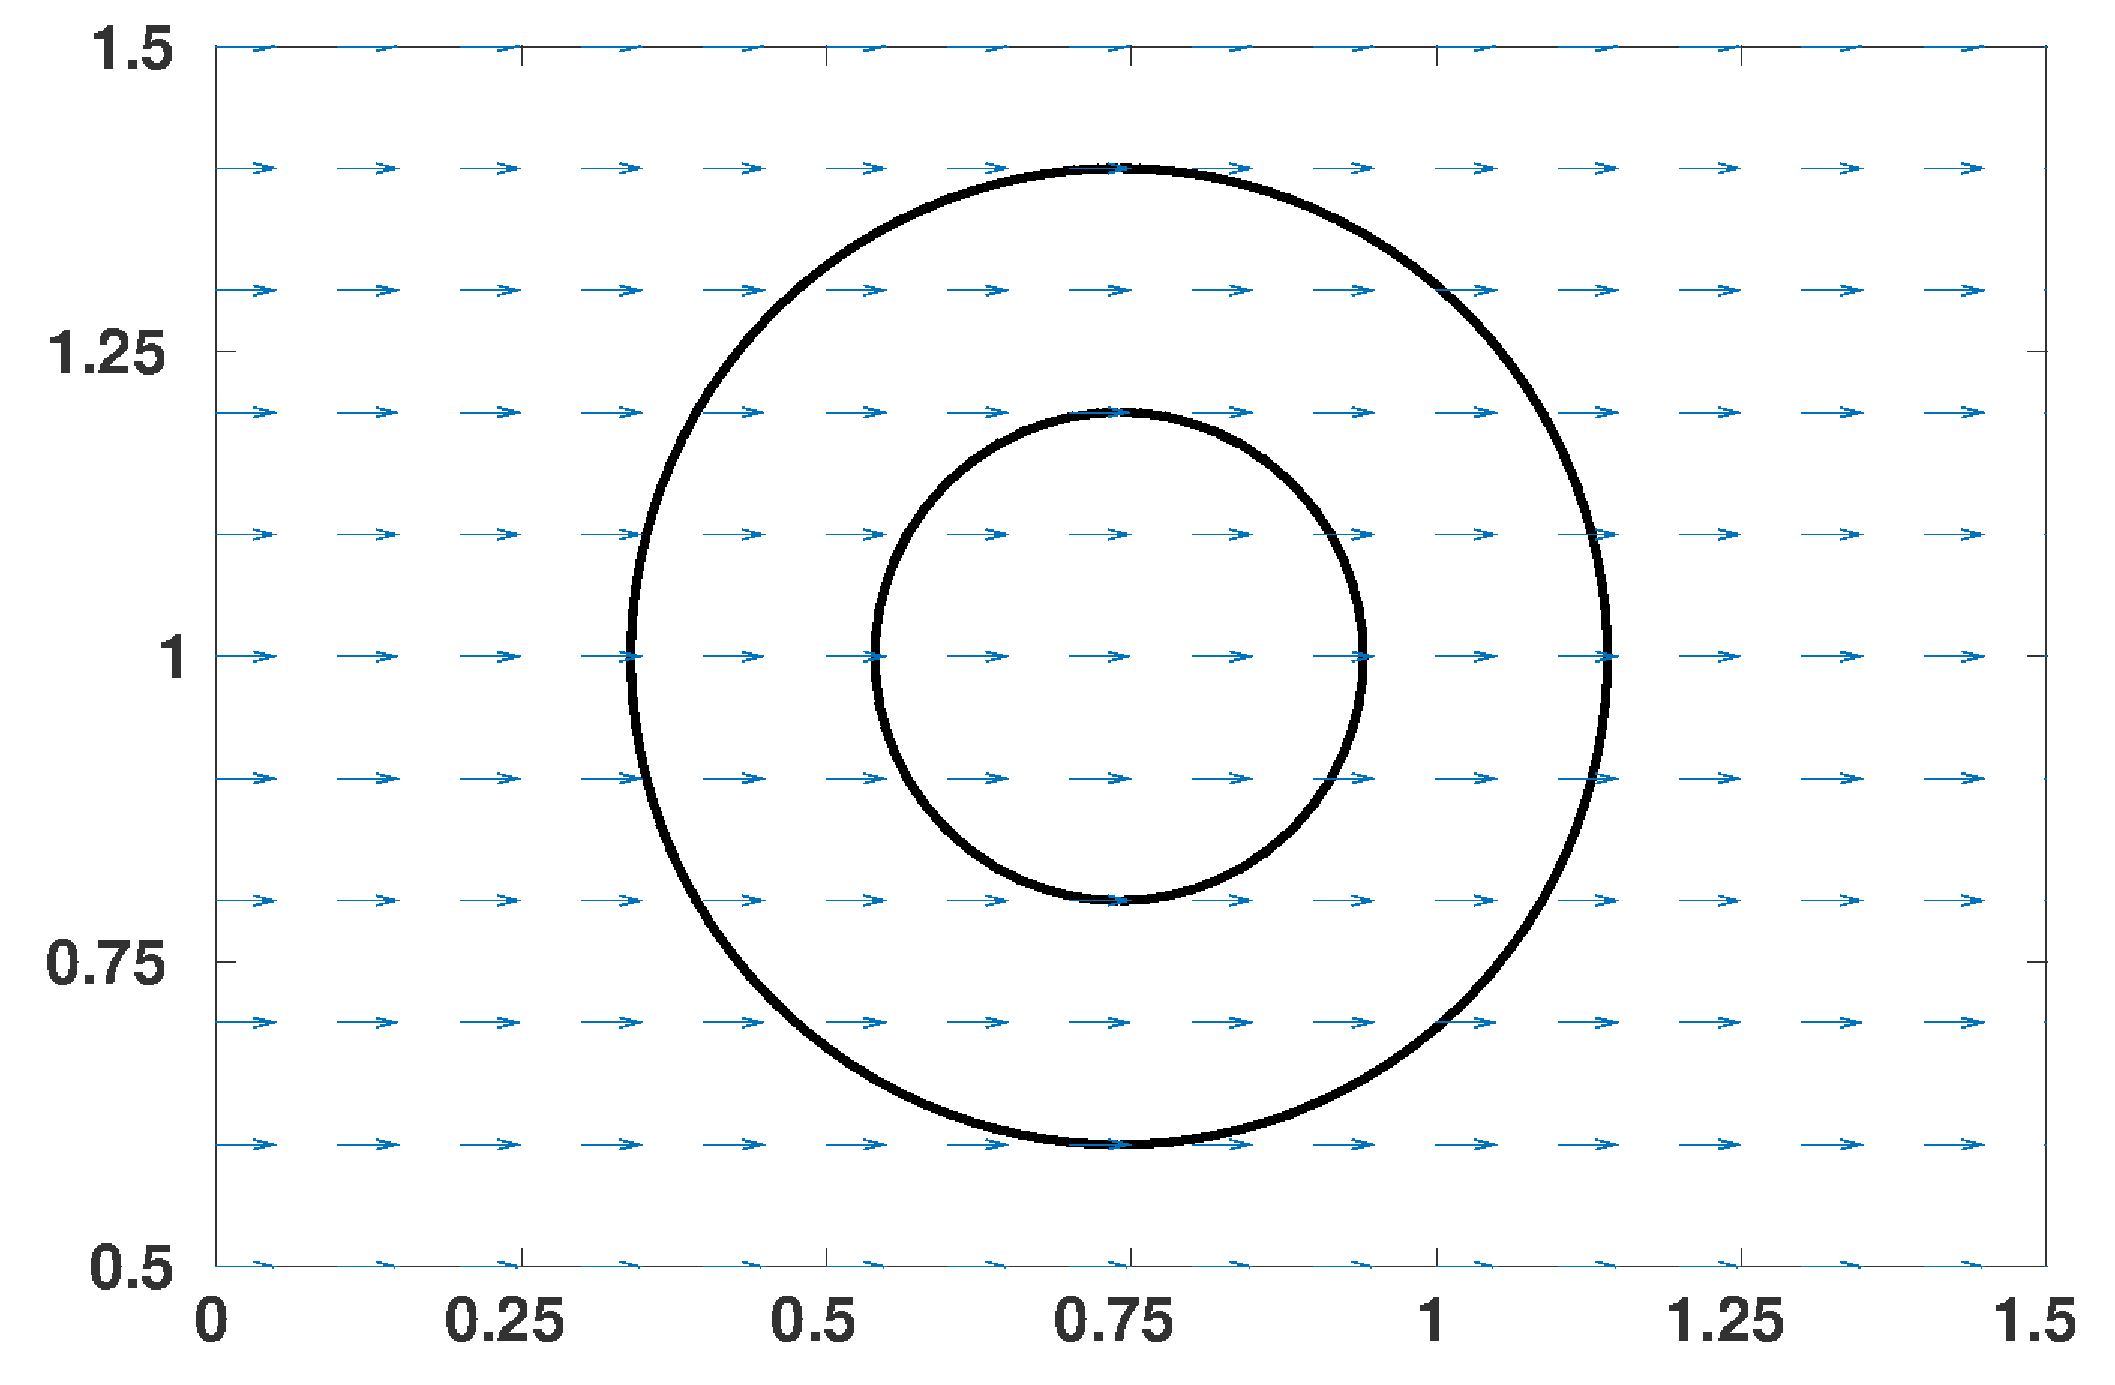
\includegraphics[width=0.5\textwidth]{IC.eps}
      }
  \subfloat[After advecting 500 steps ]{%
      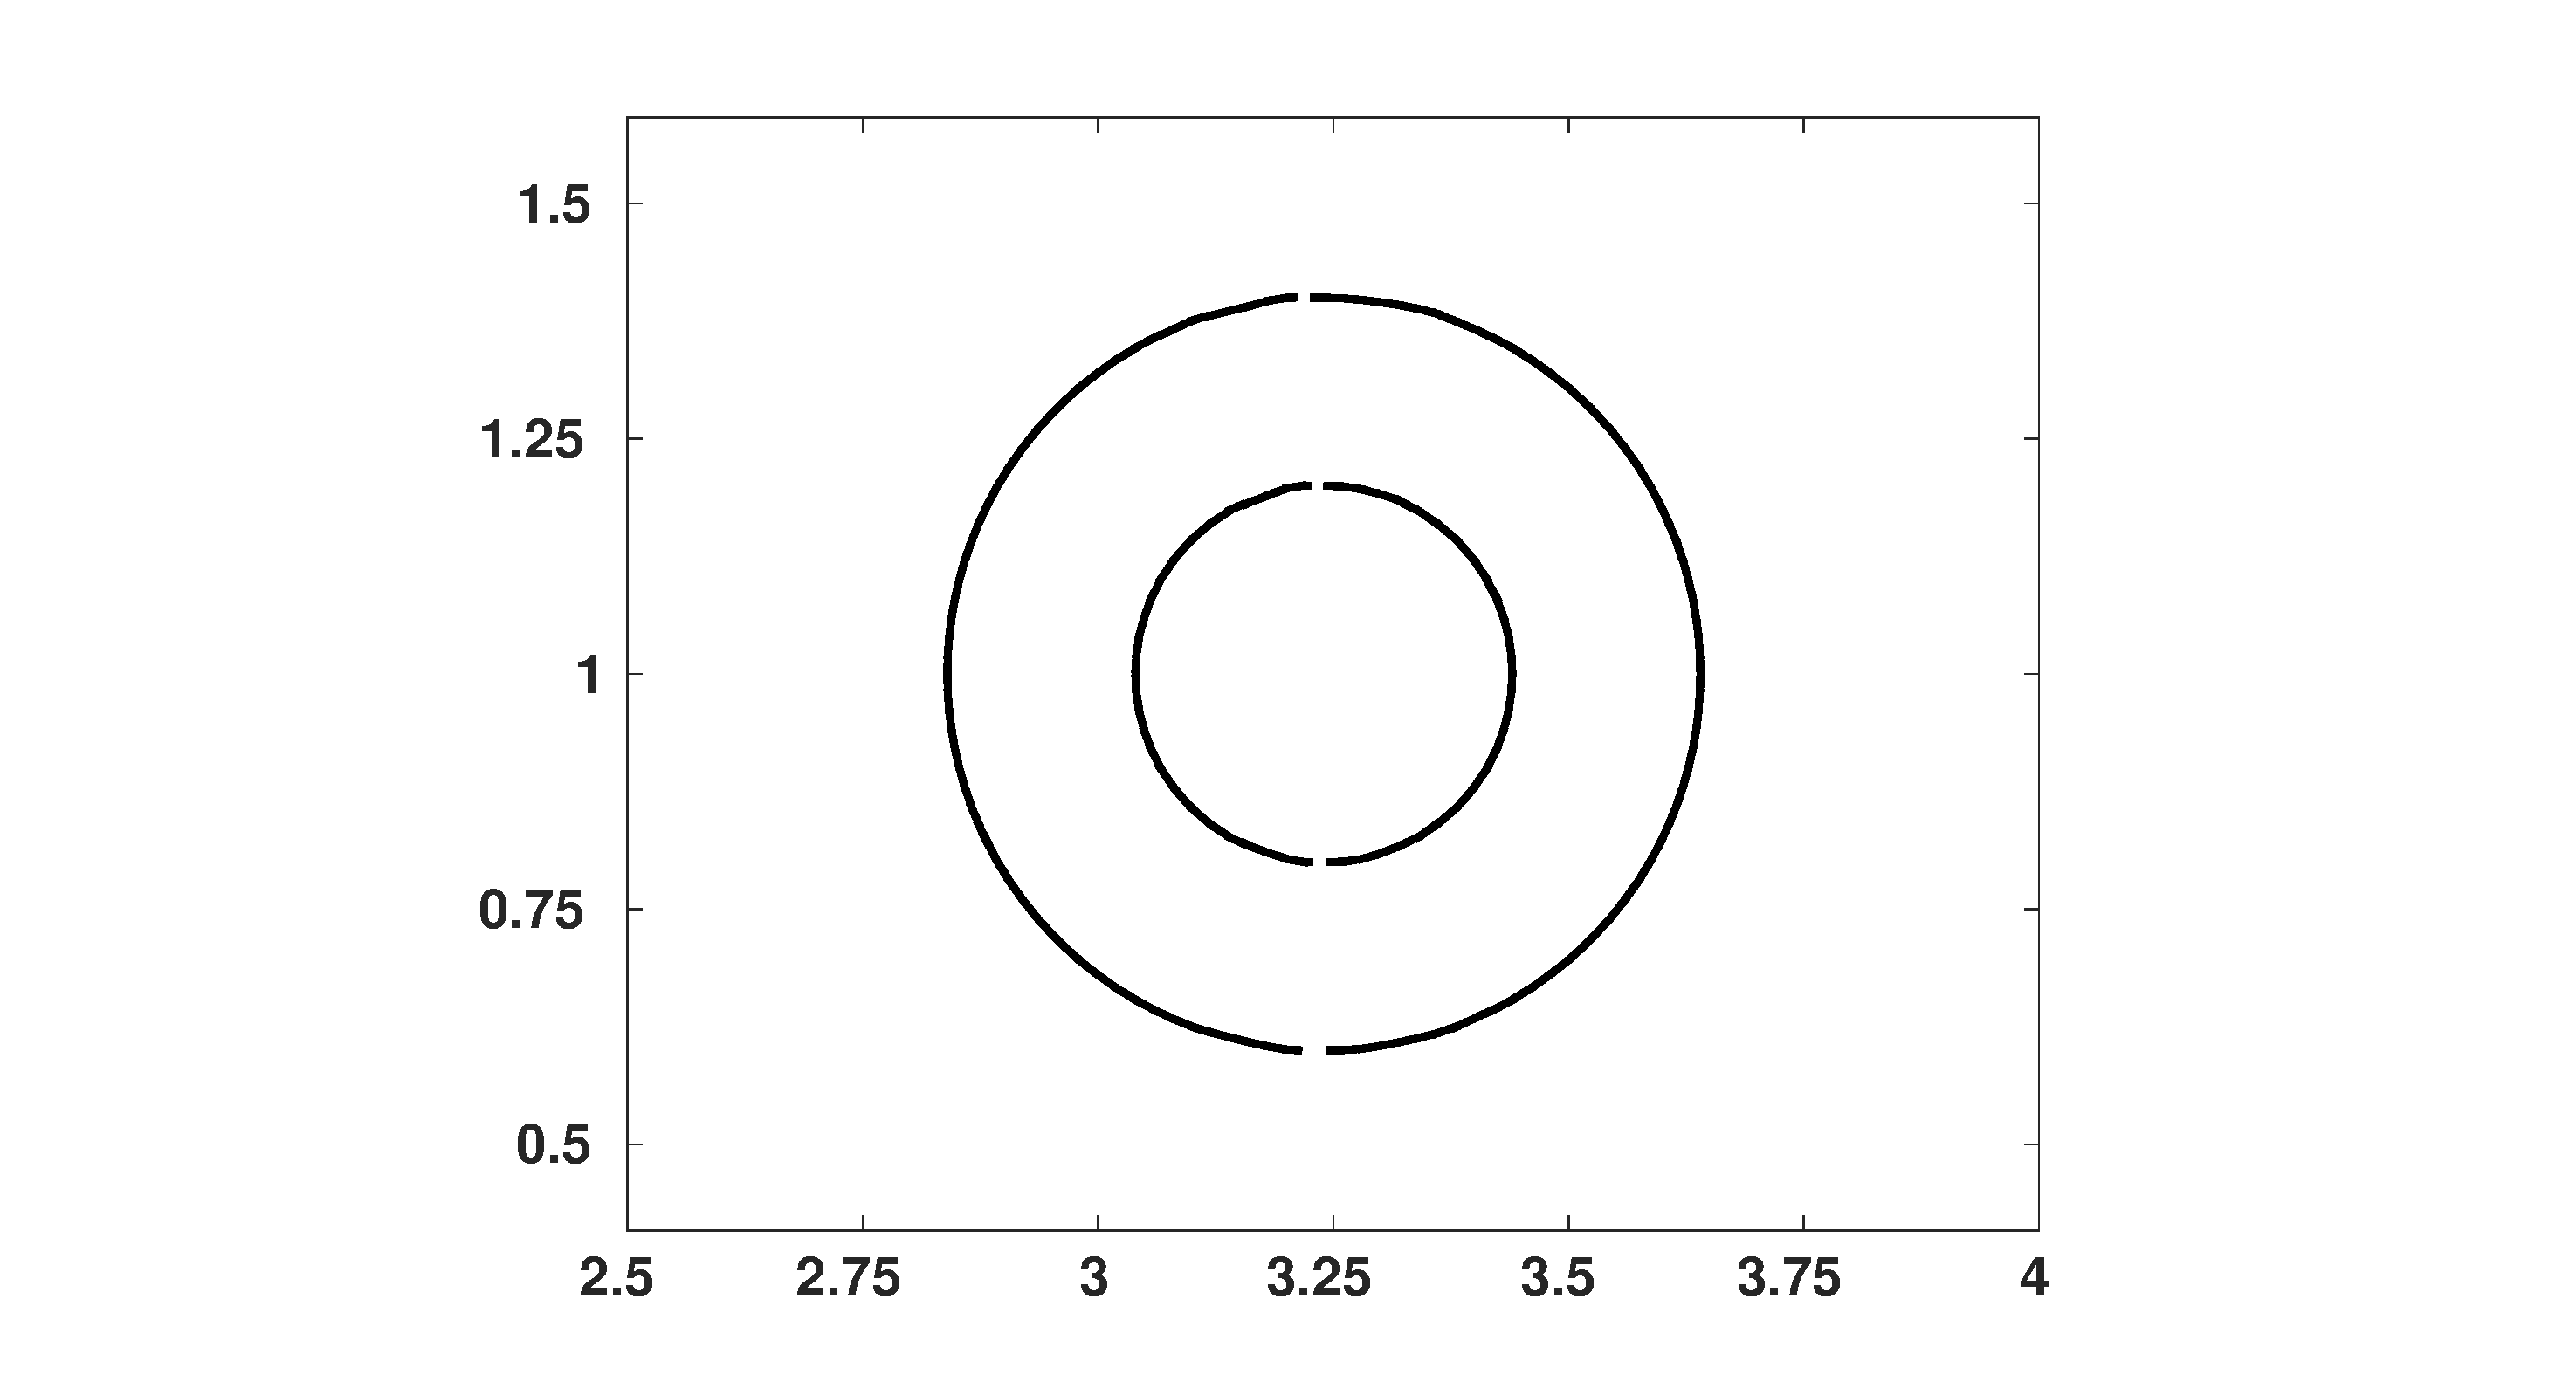
\includegraphics[width=0.5\textwidth]{final500.eps}
      }
 \caption{Advection test for velocity field u=1,v=0}
 \label{Fig:translational_test}
\end{figure}

\begin{figure}%[H]
 \centering
 \subfloat[Initial Condition for translational test ]{%
      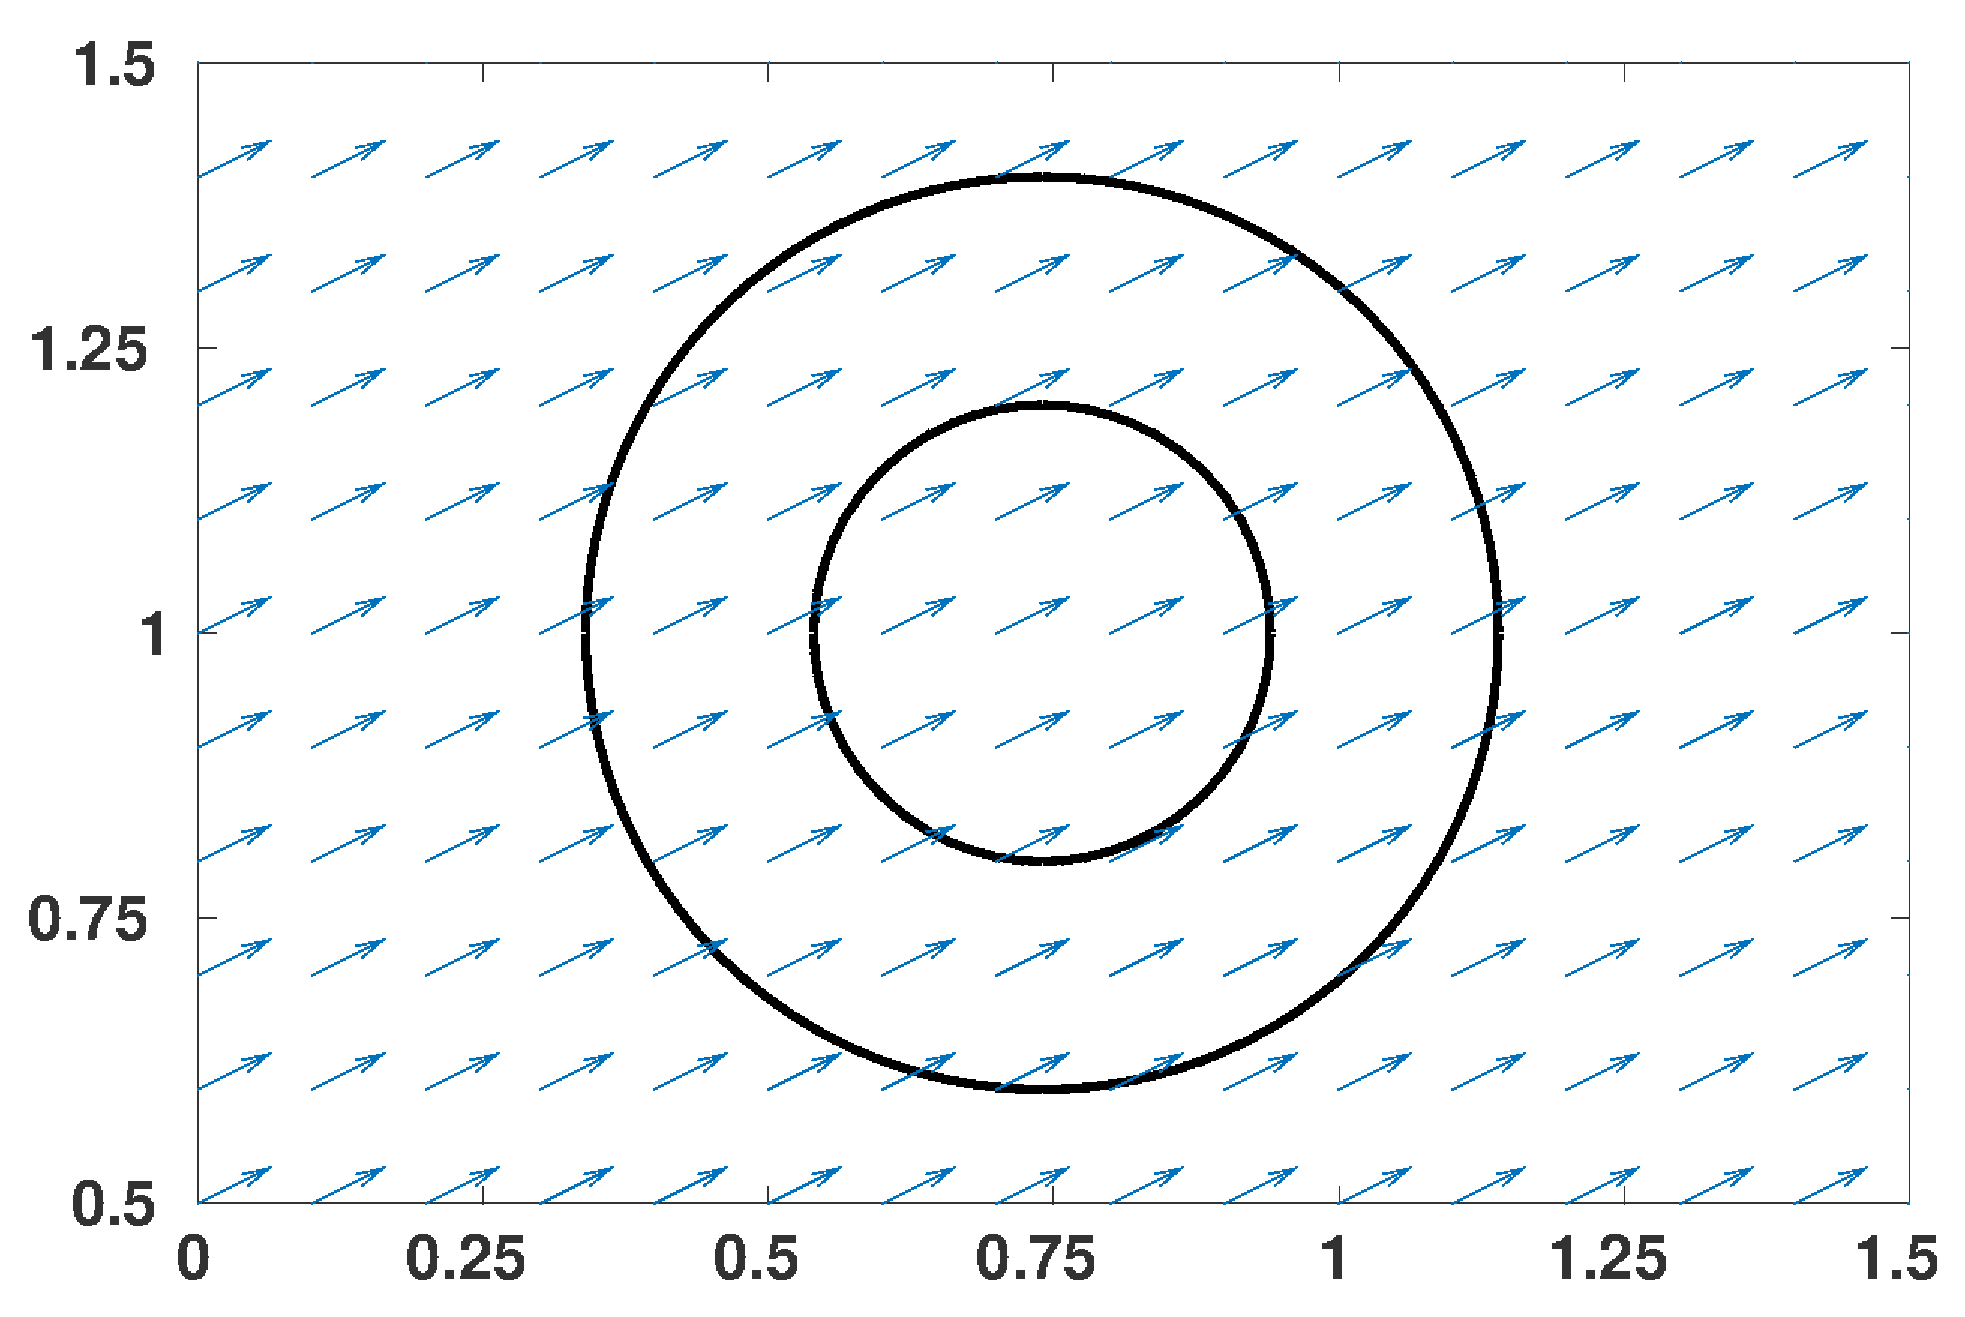
\includegraphics[width=0.5\textwidth]{IC21.eps}
      }
\subfloat[After advecting 504 steps ]{%
      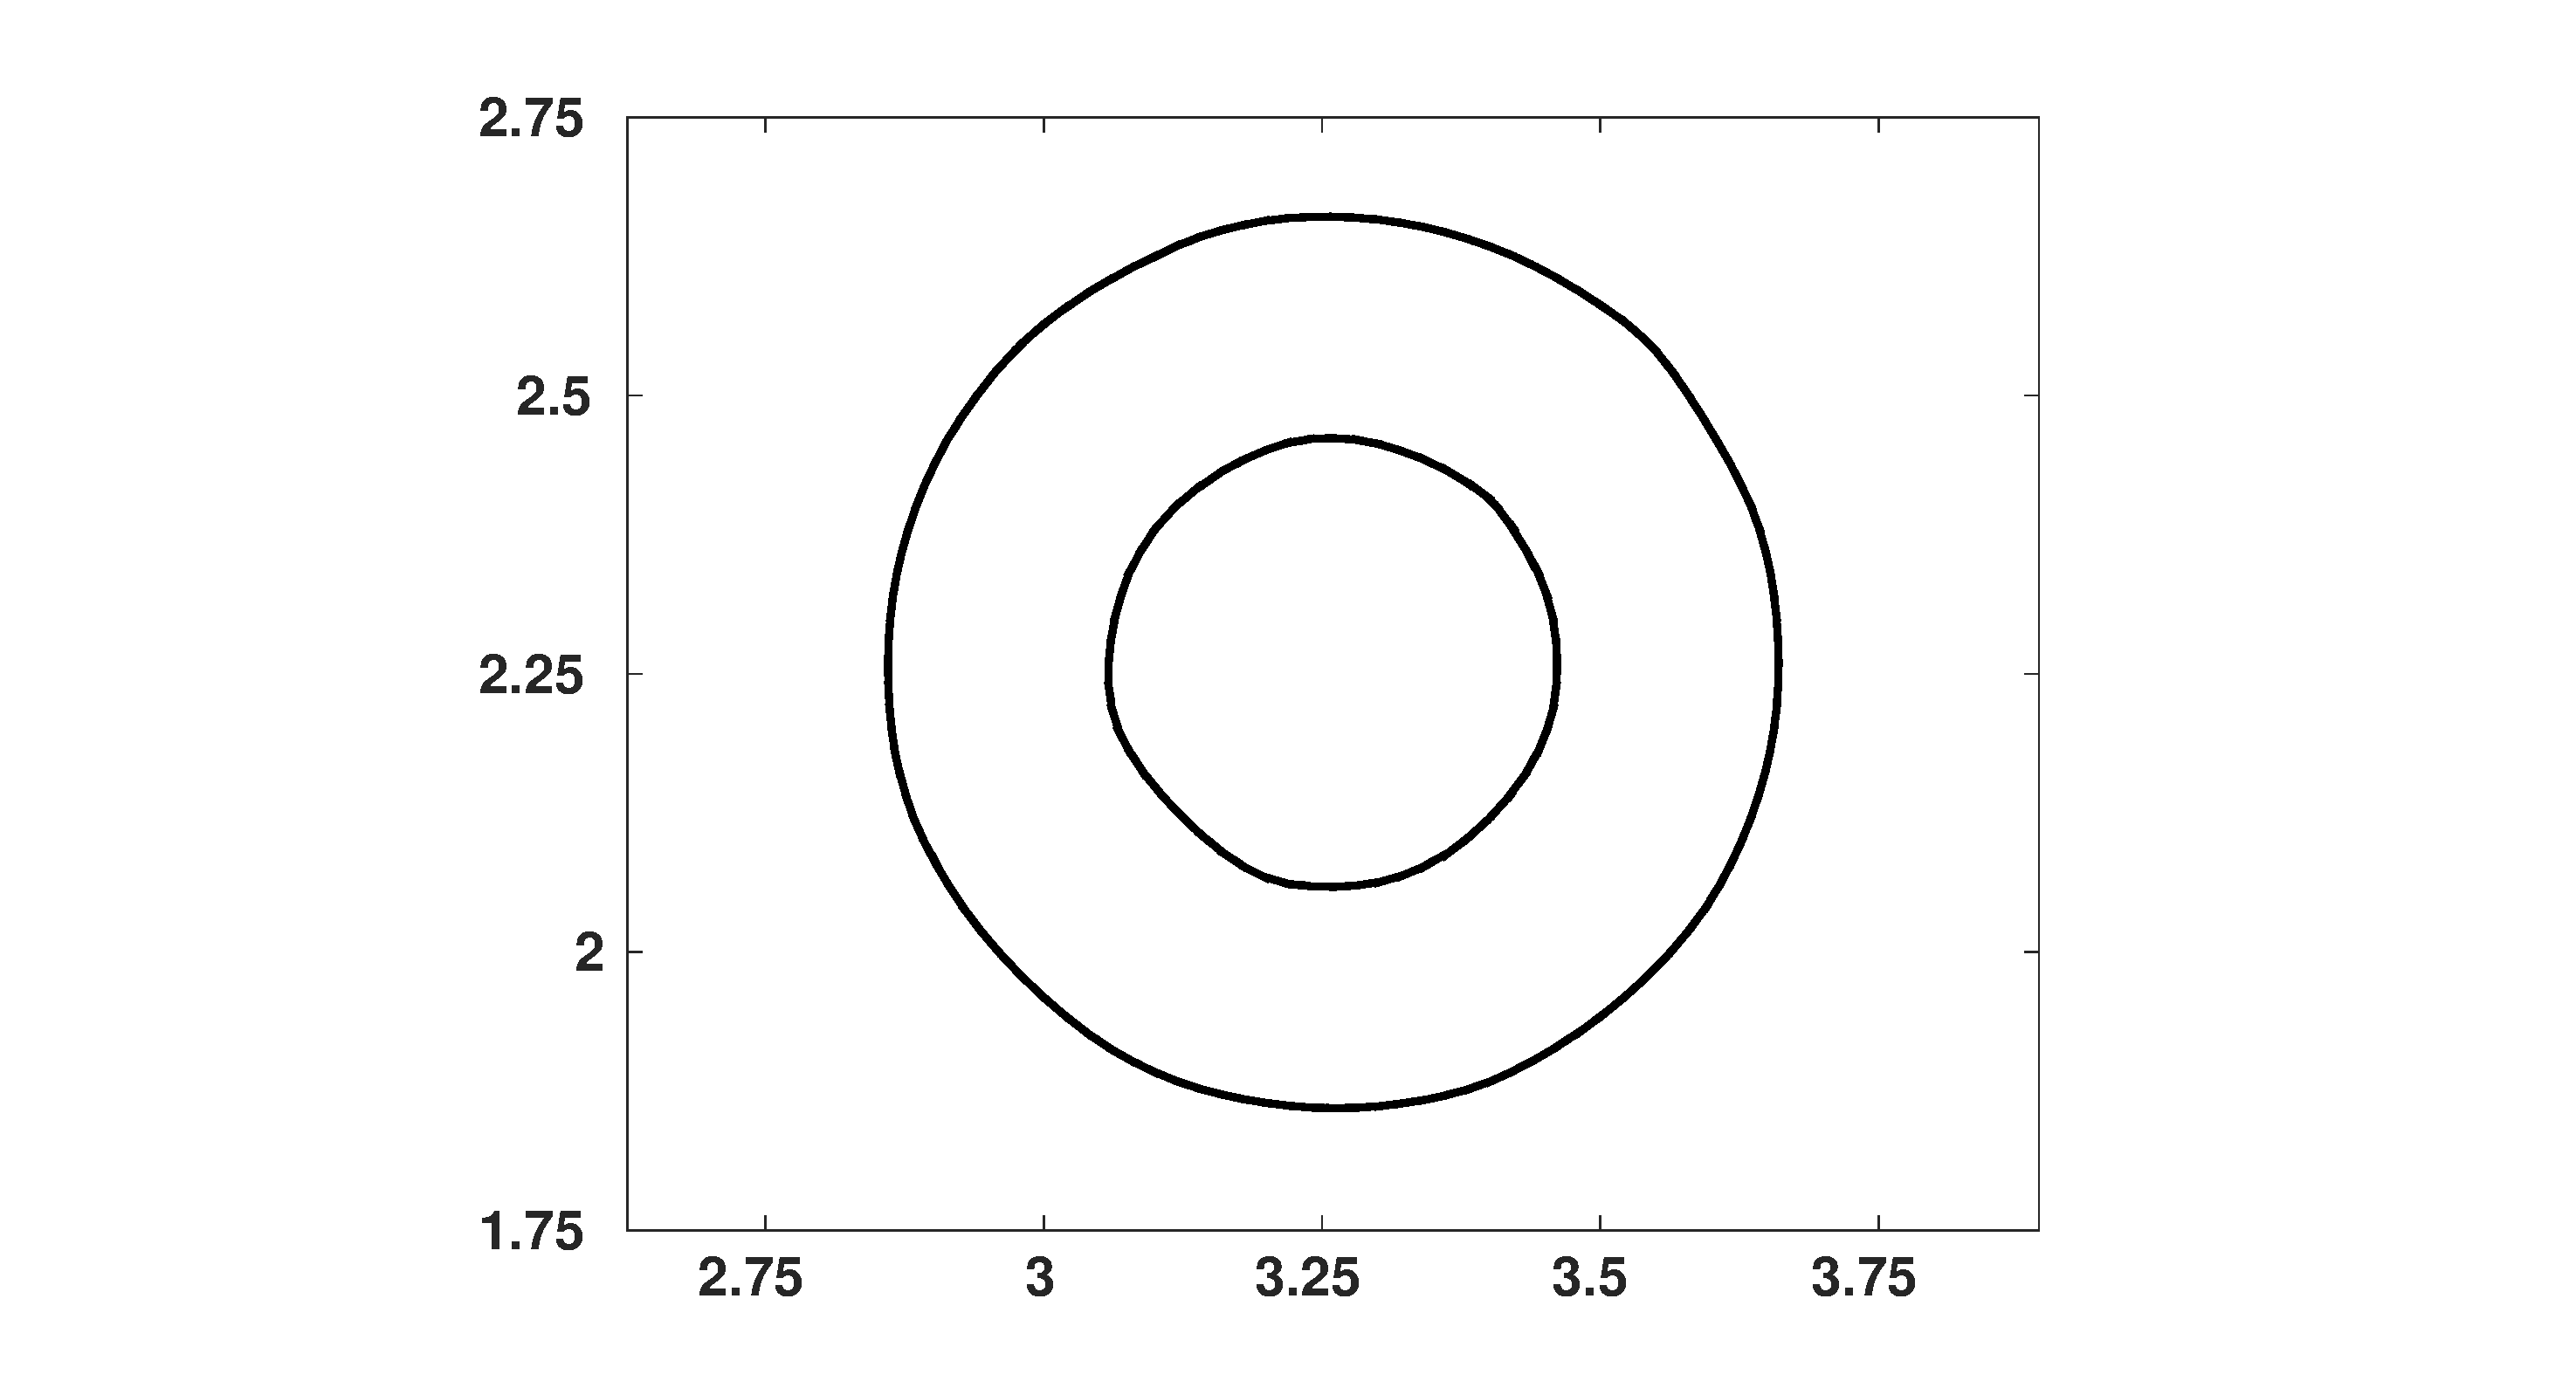
\includegraphics[width=0.5\textwidth]{final504.eps}
      }
 \caption{Advection test for velocity field u=2,v=1}
\end{figure}

\subsection{Advection test for solid body rotation}
For solid body rotation test a slotted circle configuration is taken from \cite{Zalesak1979}, the center of slotted circle is at
(2.0,2.75) and diameter is 1.0. The length and width of slot is 0.6 and 0.12 respectively.(Figure \ref{Fig:rotation} and \ref{Fig:rotation2})  
The refinement of the domain which is [0,4] x [0,4] is 200 x 200 . A velocity field is given by $u=-\Omega(y-y_0),v=\Omega(x-x_0)$, 
where axis of rotation passes through the $(x_0,y_0)$ and normal to the x-y plane. $\Omega$ is the angular velocity. 
Here $\Omega = 0.5$ and $(x_0,y_0)$ is $(2,2)$. The time step is 0.005.
\begin{enumerate}
 \item Domain: [0,4] x [0,4]
 \item Grid Size: 200 x 200
 \item Radius of circle :0.5
 \item Center : (2.0,2.75)
 \item Velocity field:  $u=-0.5(y-2),v=0.5(x-2)$
\end{enumerate}

% 
\begin{figure}
  \subfloat[After advecting 628 steps ]{%
      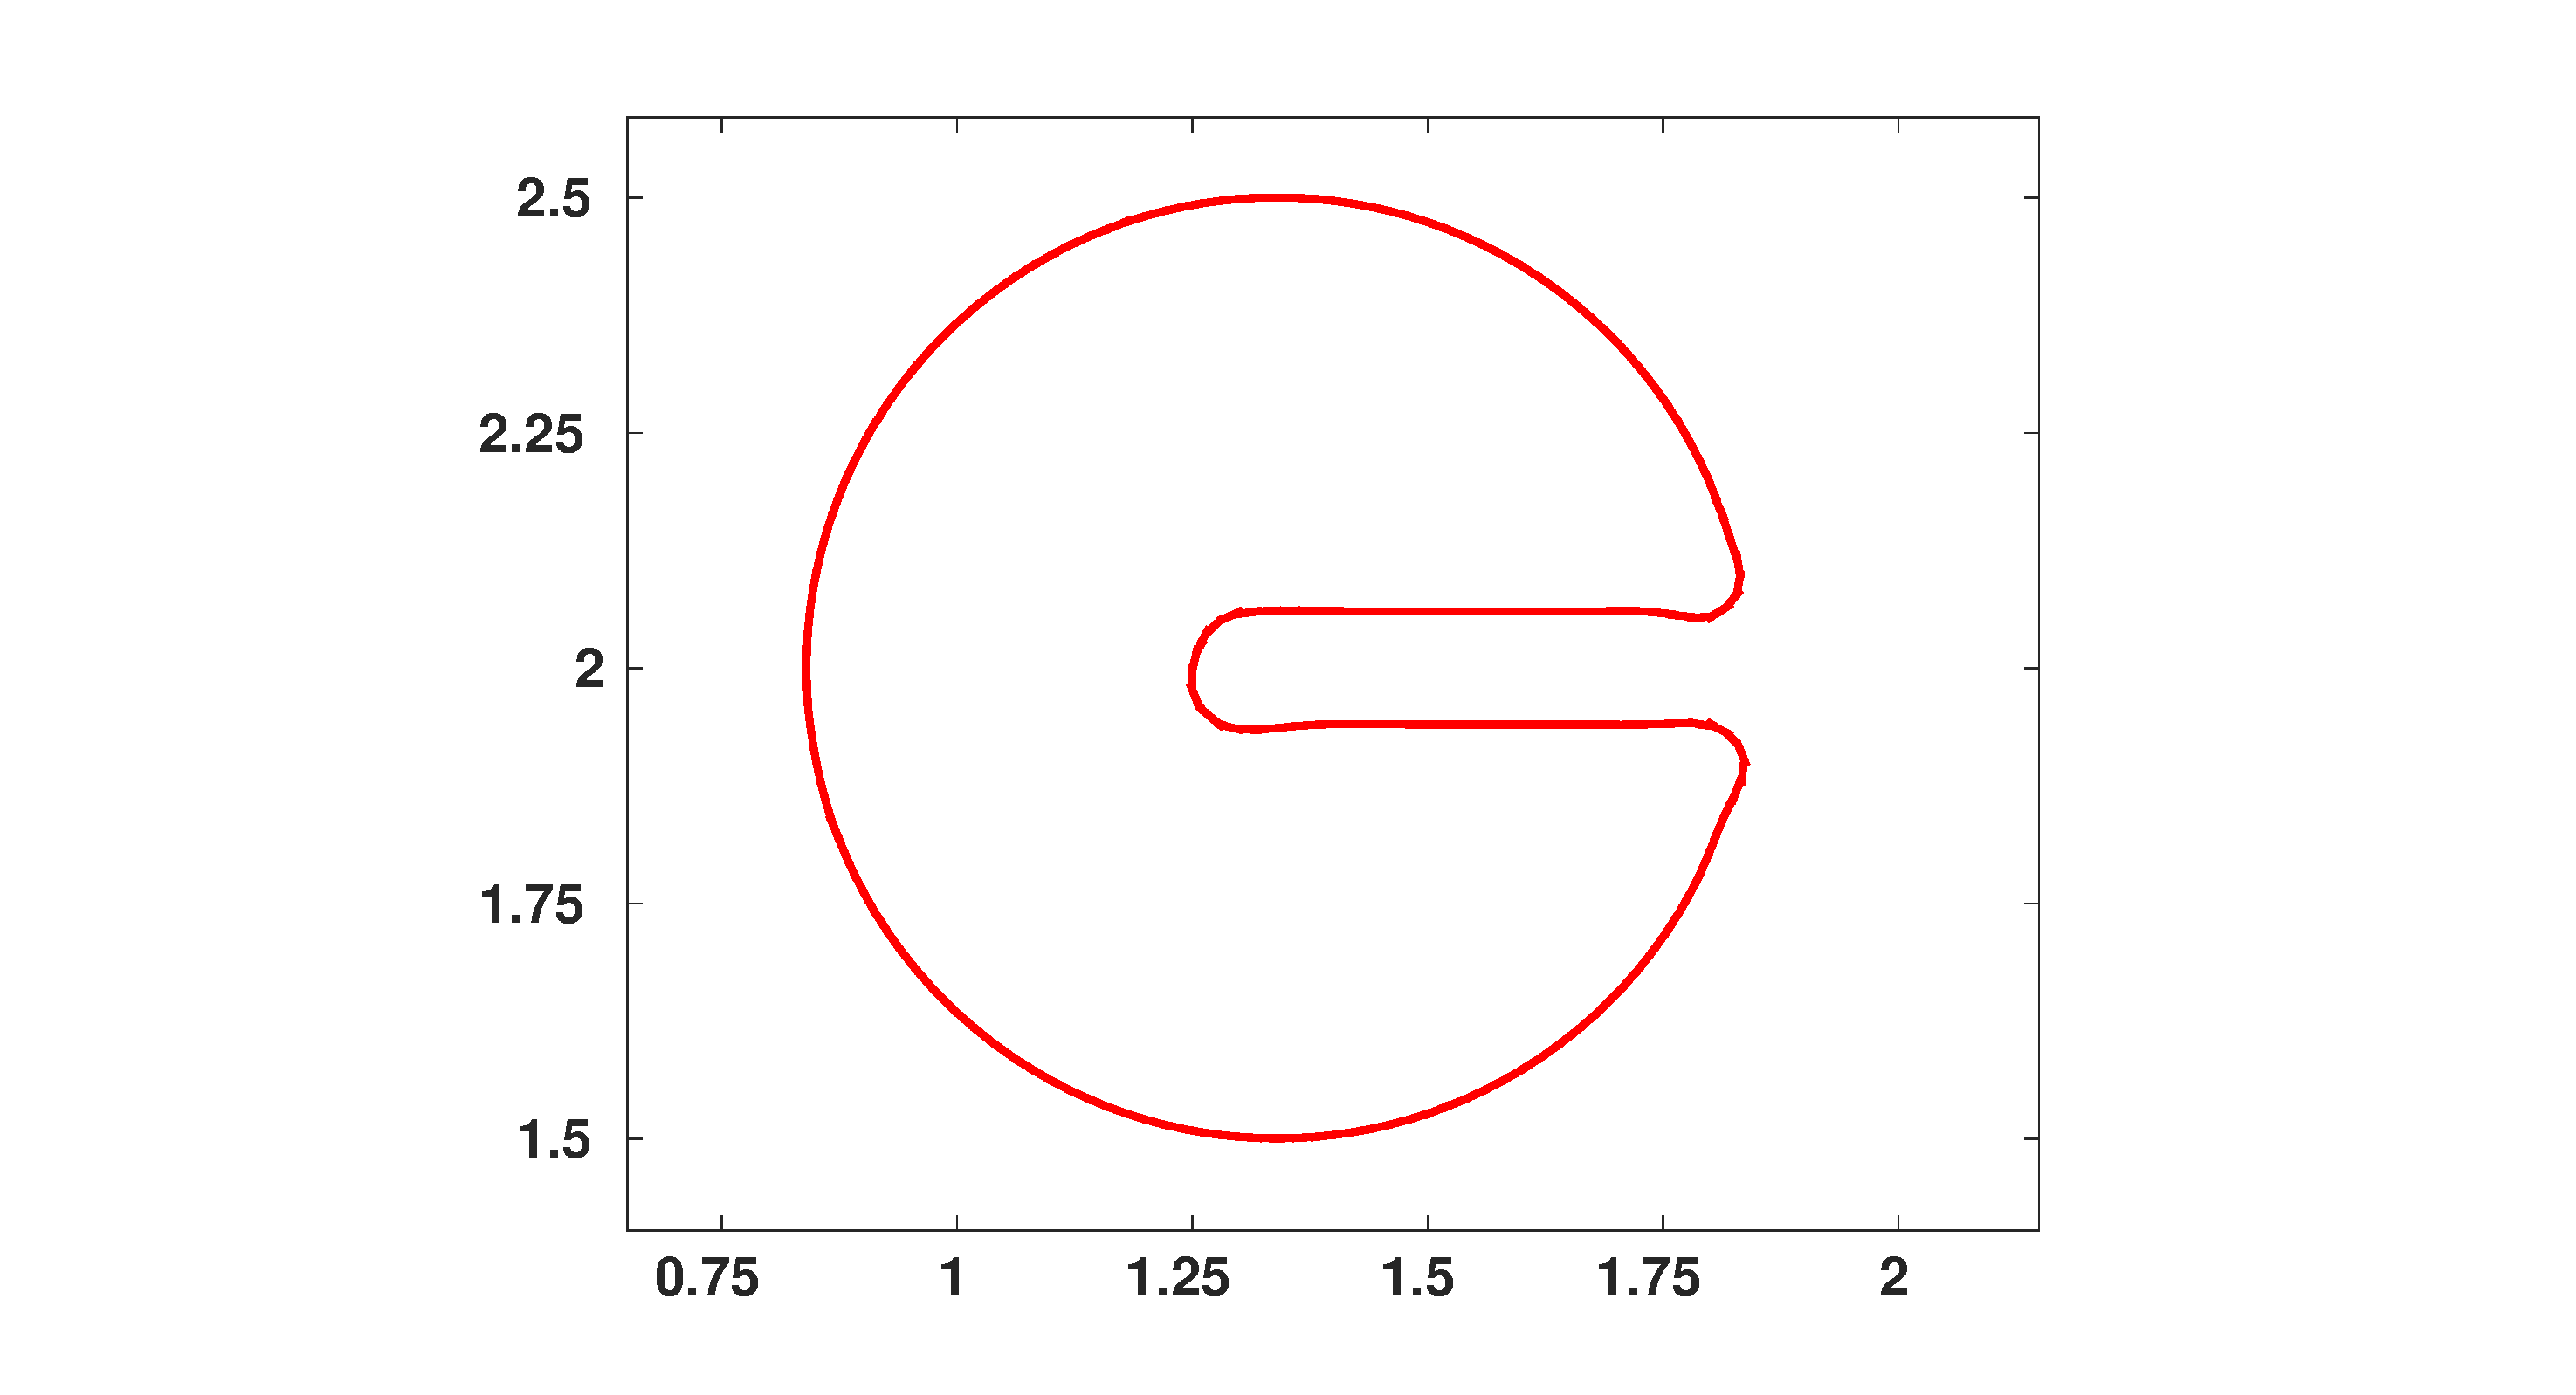
\includegraphics[width=0.5\textwidth]{SC_628.eps}
      }
     \subfloat[After advecting 1256 steps ]{%
      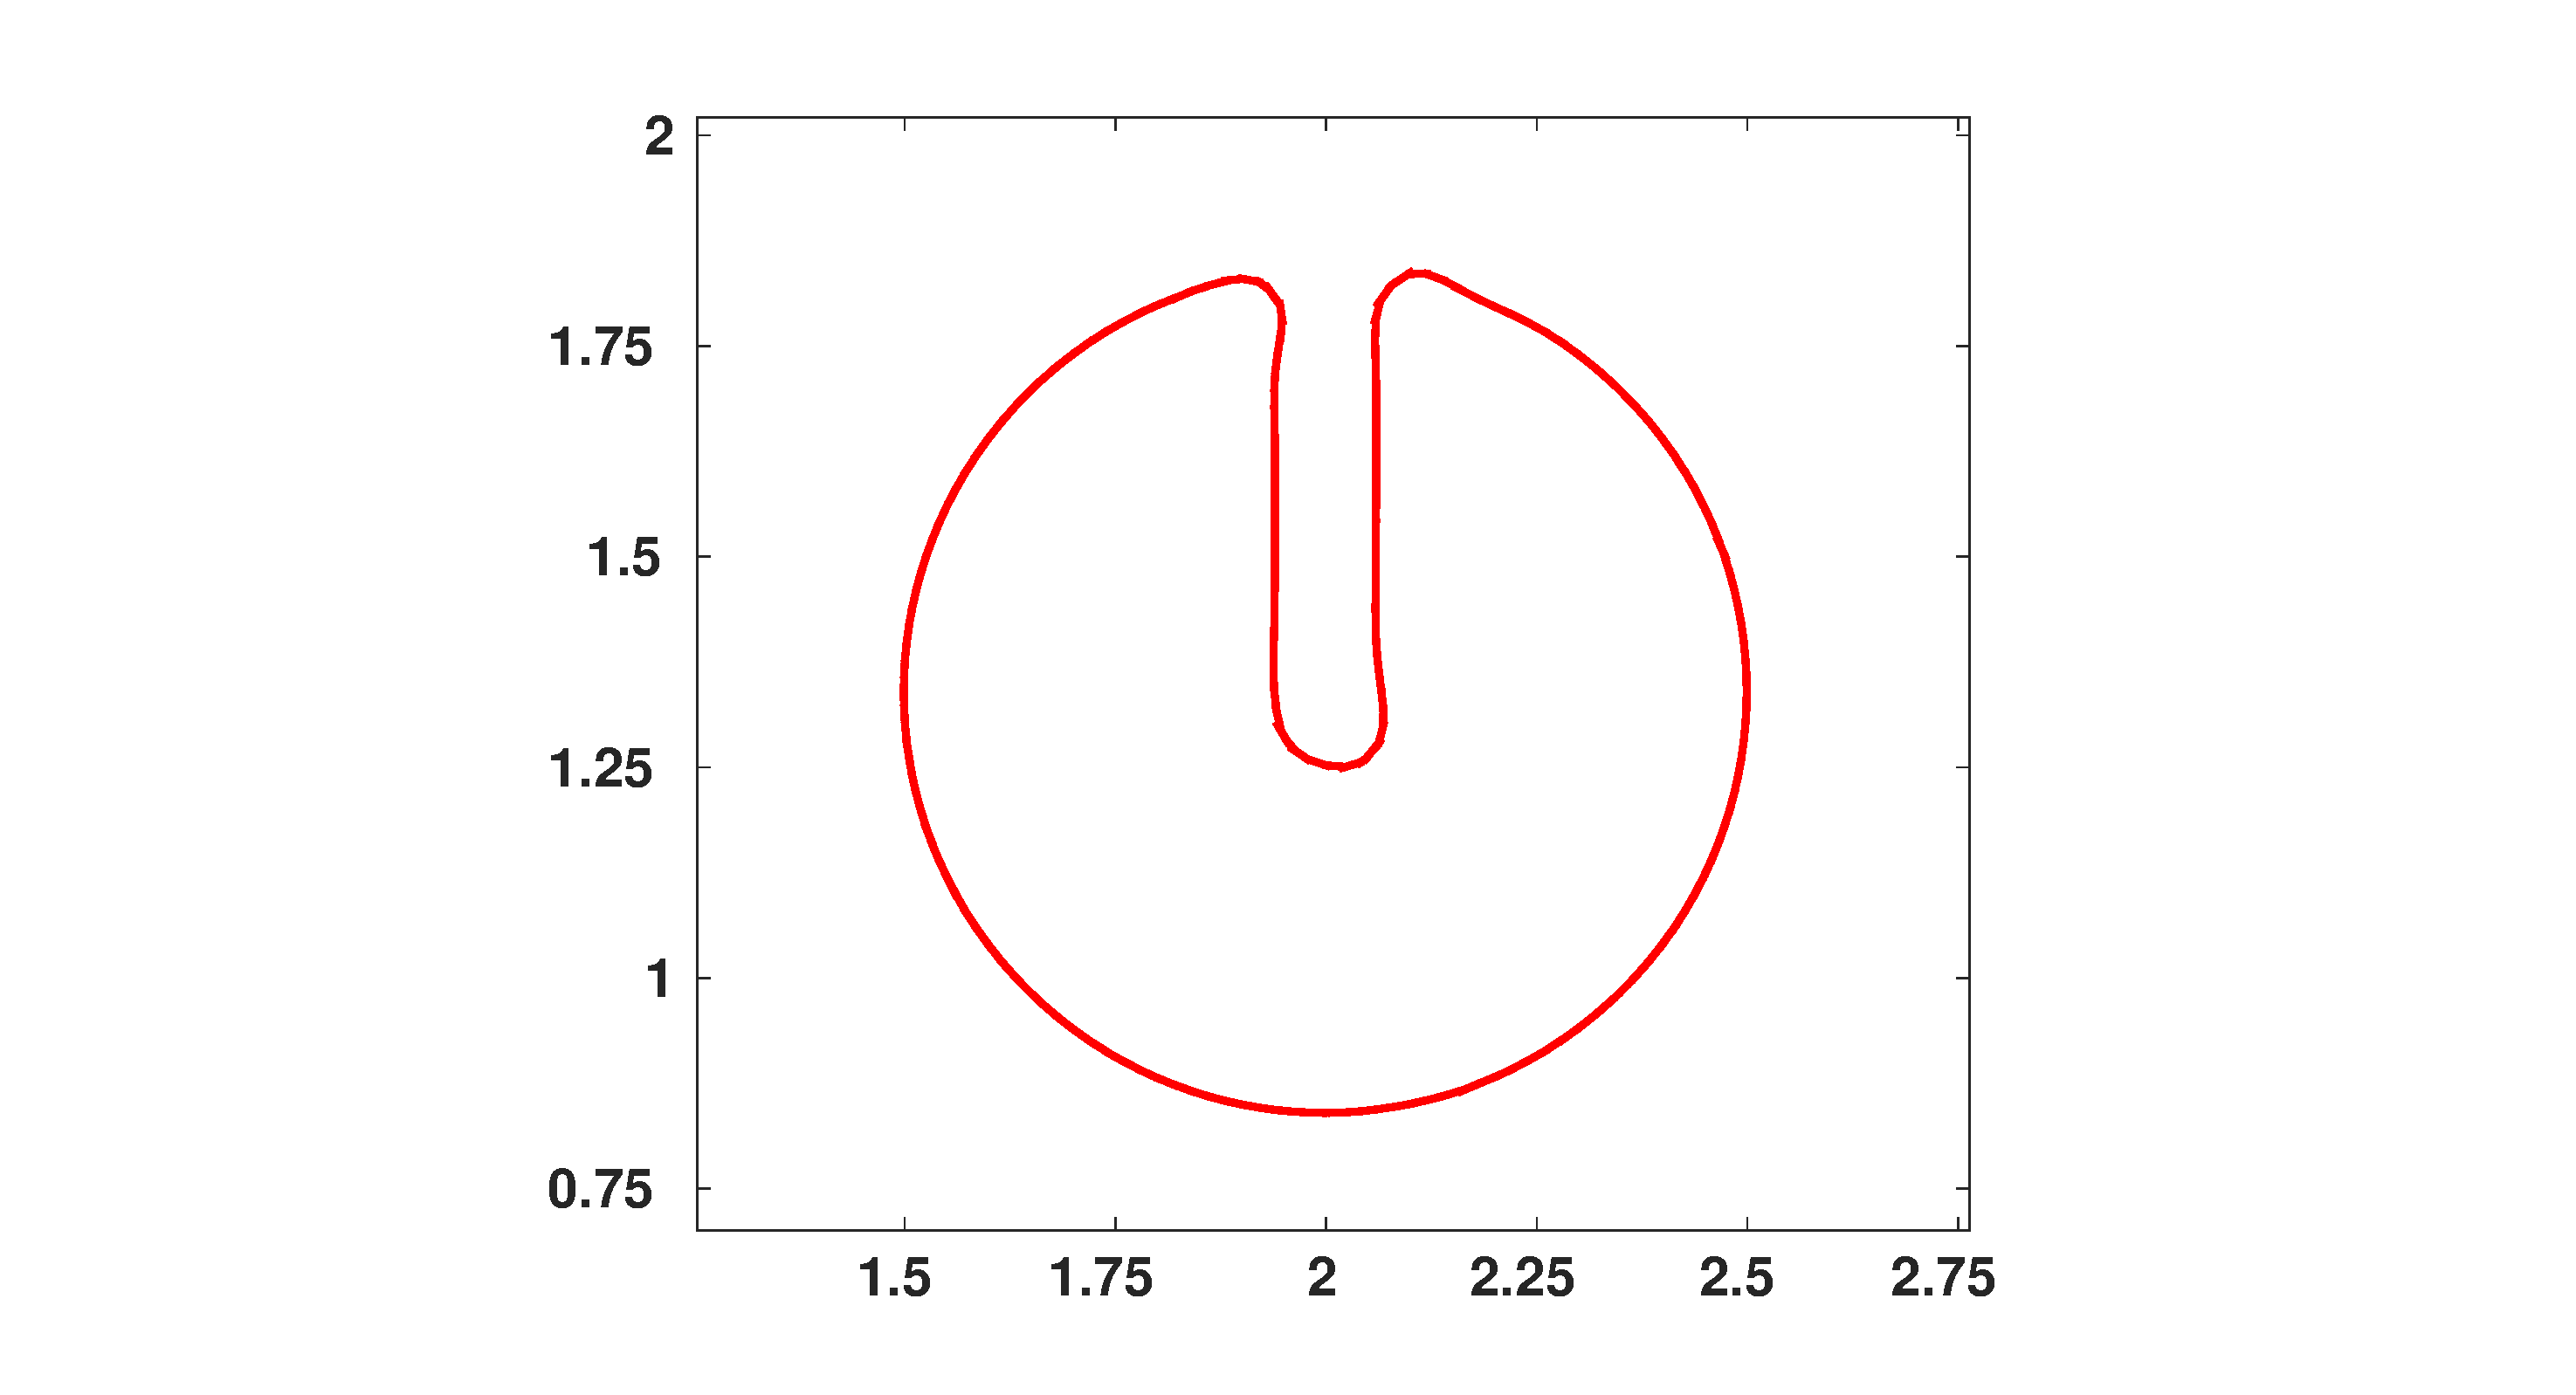
\includegraphics[width=0.5\textwidth]{SC_1256.eps}
      }\\
        \subfloat[After advecting 1885 steps ]{%
      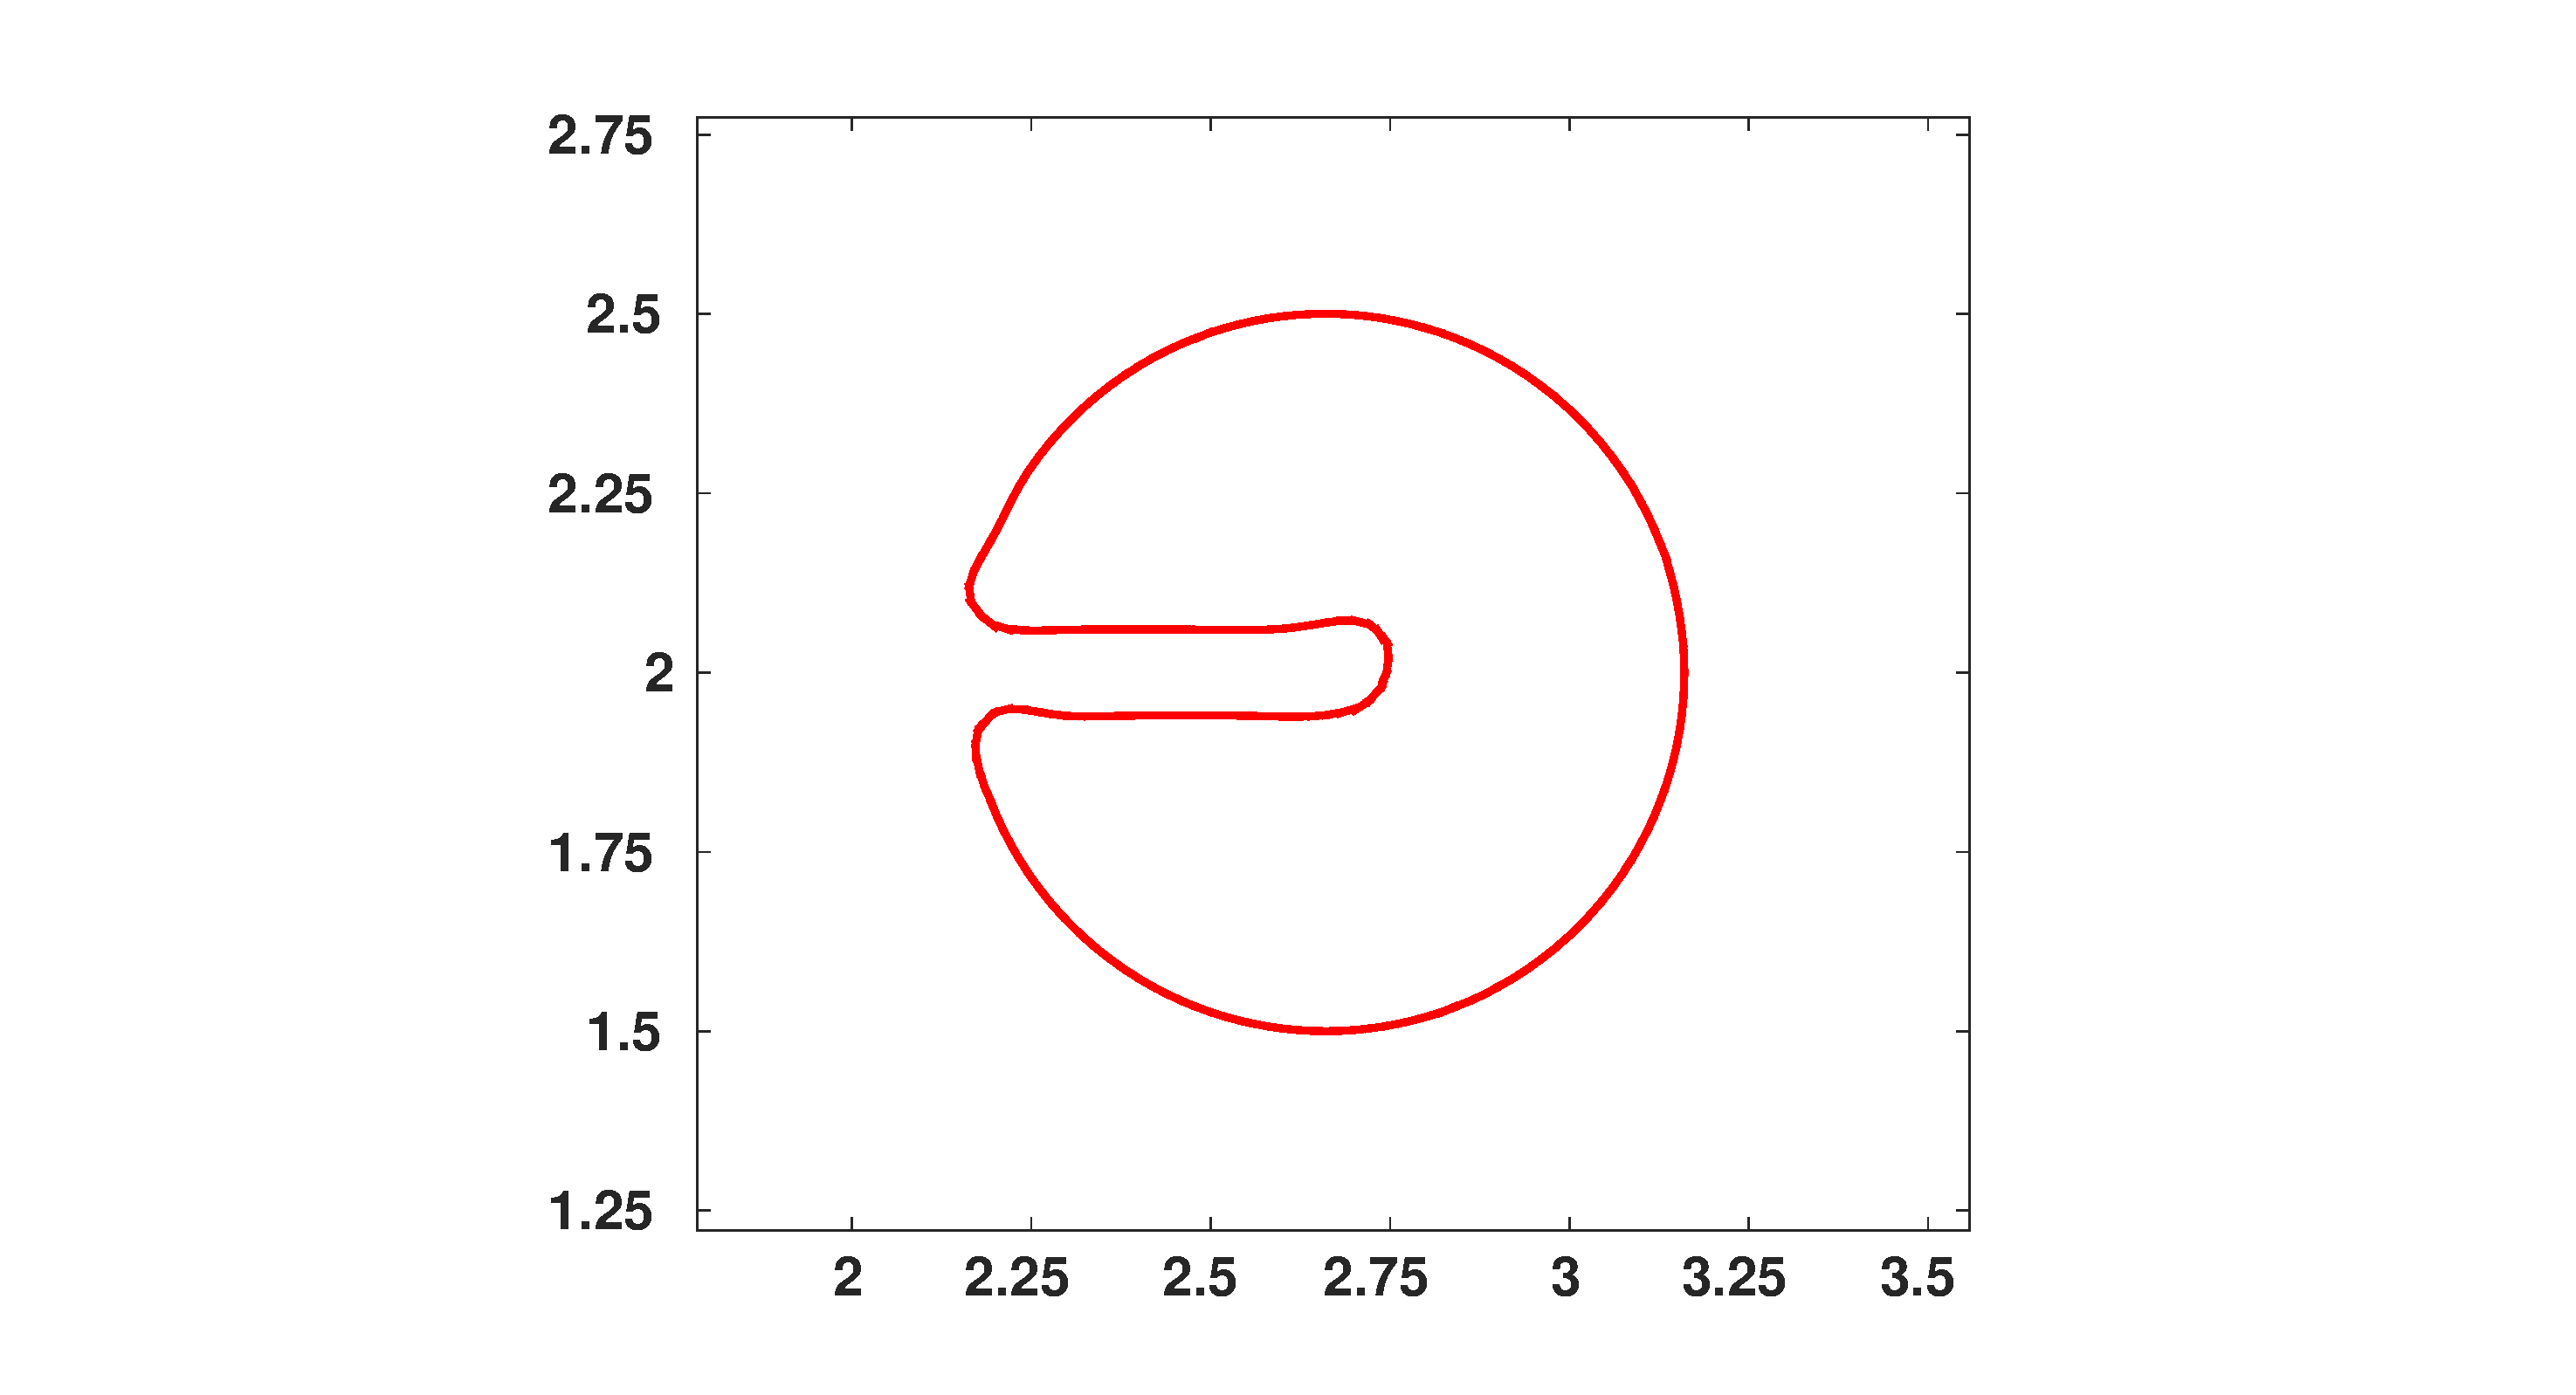
\includegraphics[width=0.5\textwidth]{SC_1885.eps}
      }
        \subfloat[After advecting 2513 steps ]{%
      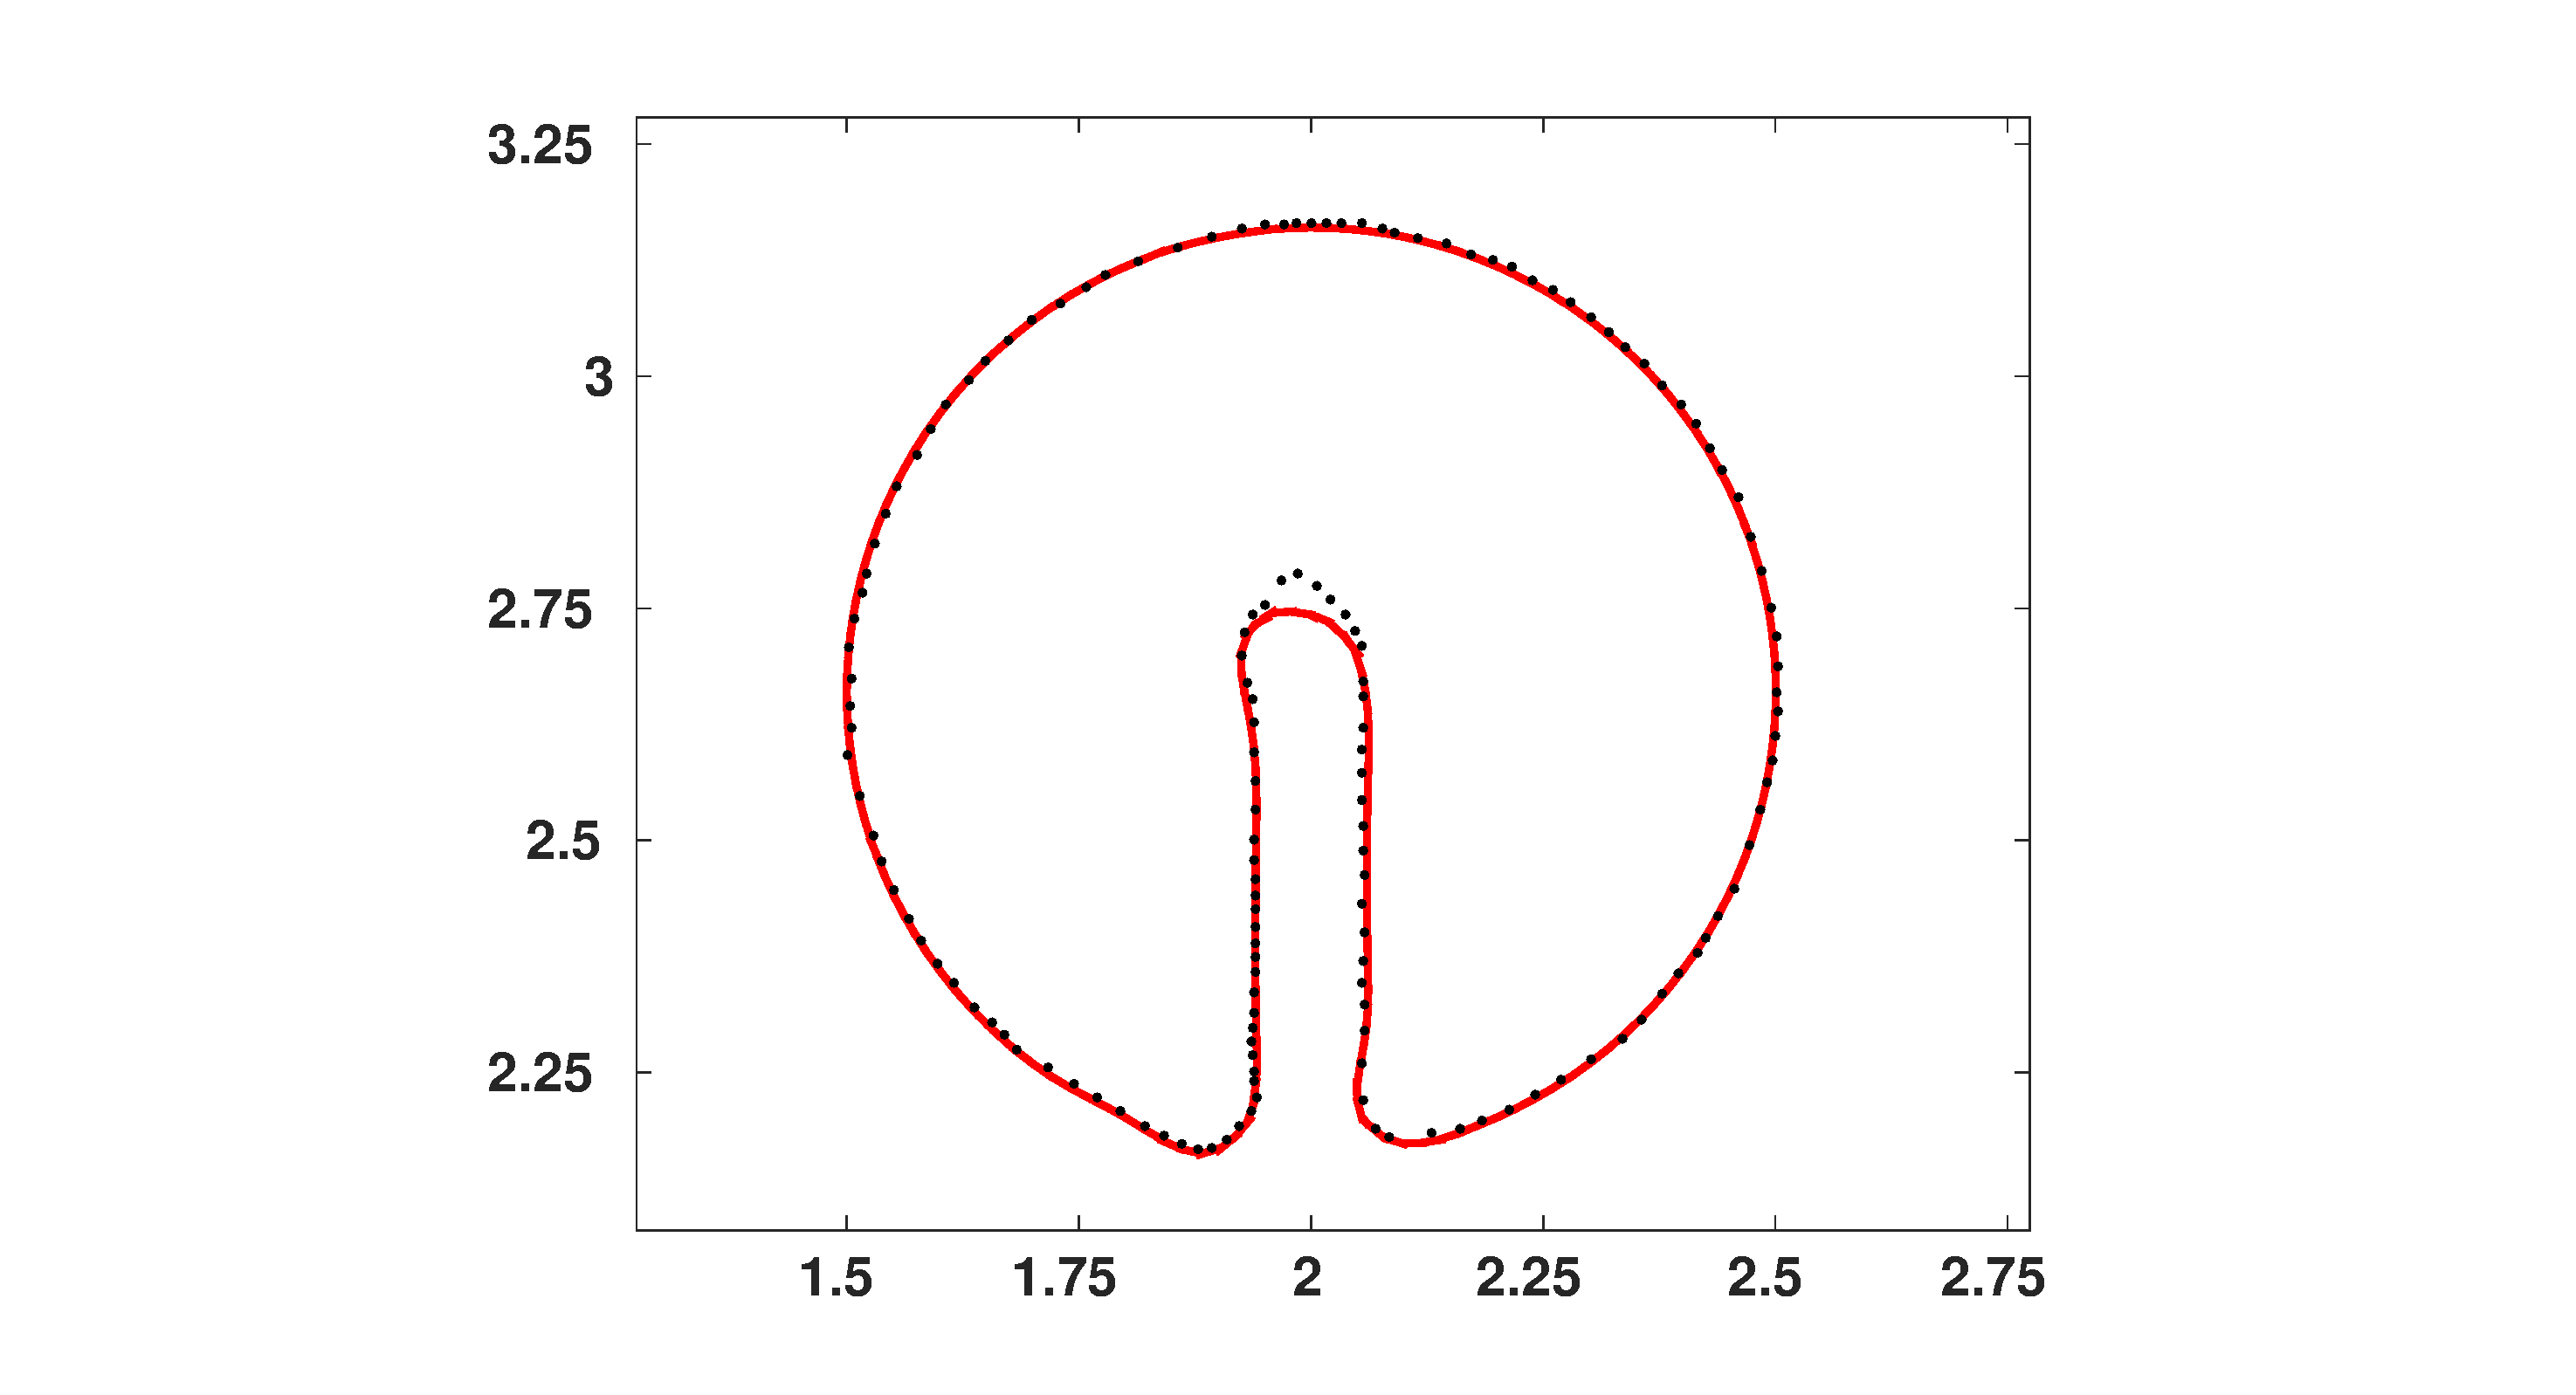
\includegraphics[width=0.5\textwidth]{SC_2513.eps}
      }
 \caption{Advection test result for solid body rotation}
 \label{Fig:rotation2}
\end{figure}
% 
\begin{figure}
 \centering 
 \subfloat[Initial Condition for solid body rotation test ]{%
      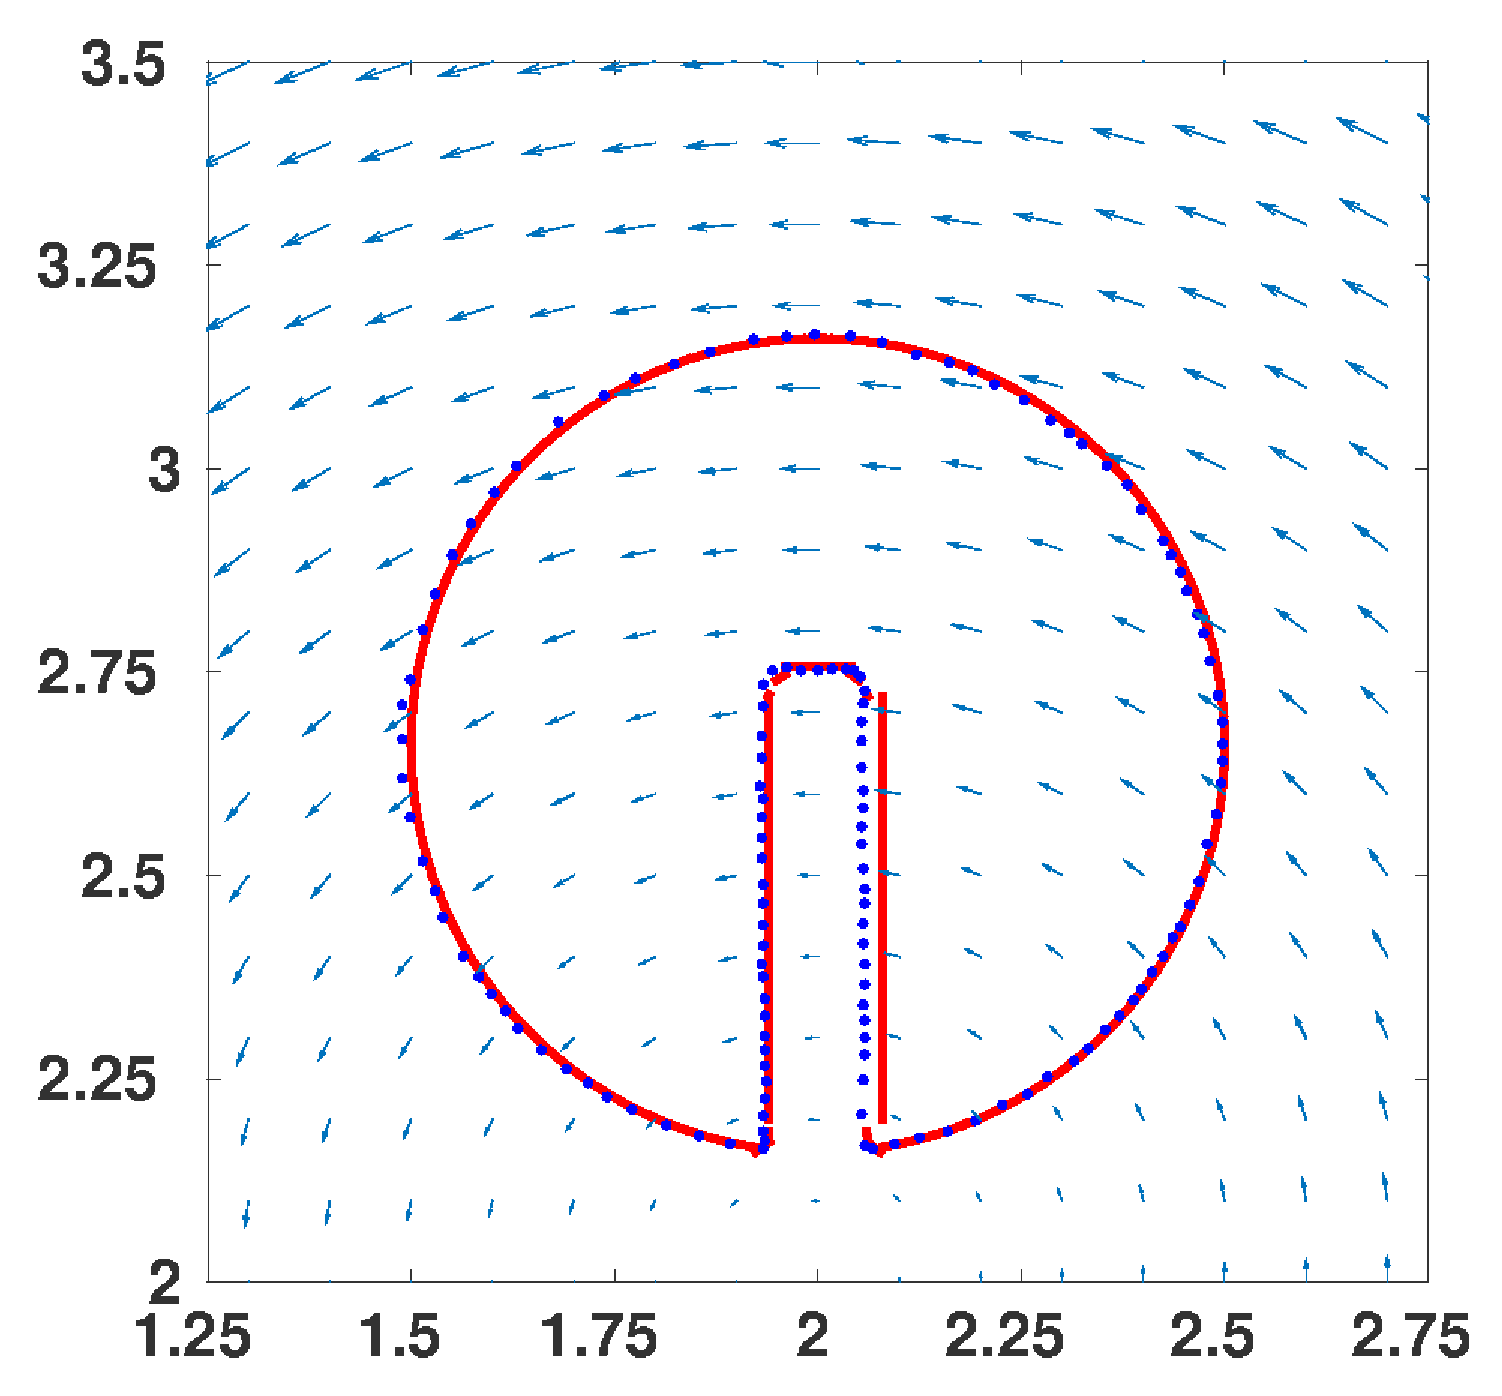
\includegraphics[width=0.5\textwidth]{SC_IC.eps}
      } 
  \subfloat[After one full rotation ]{%
      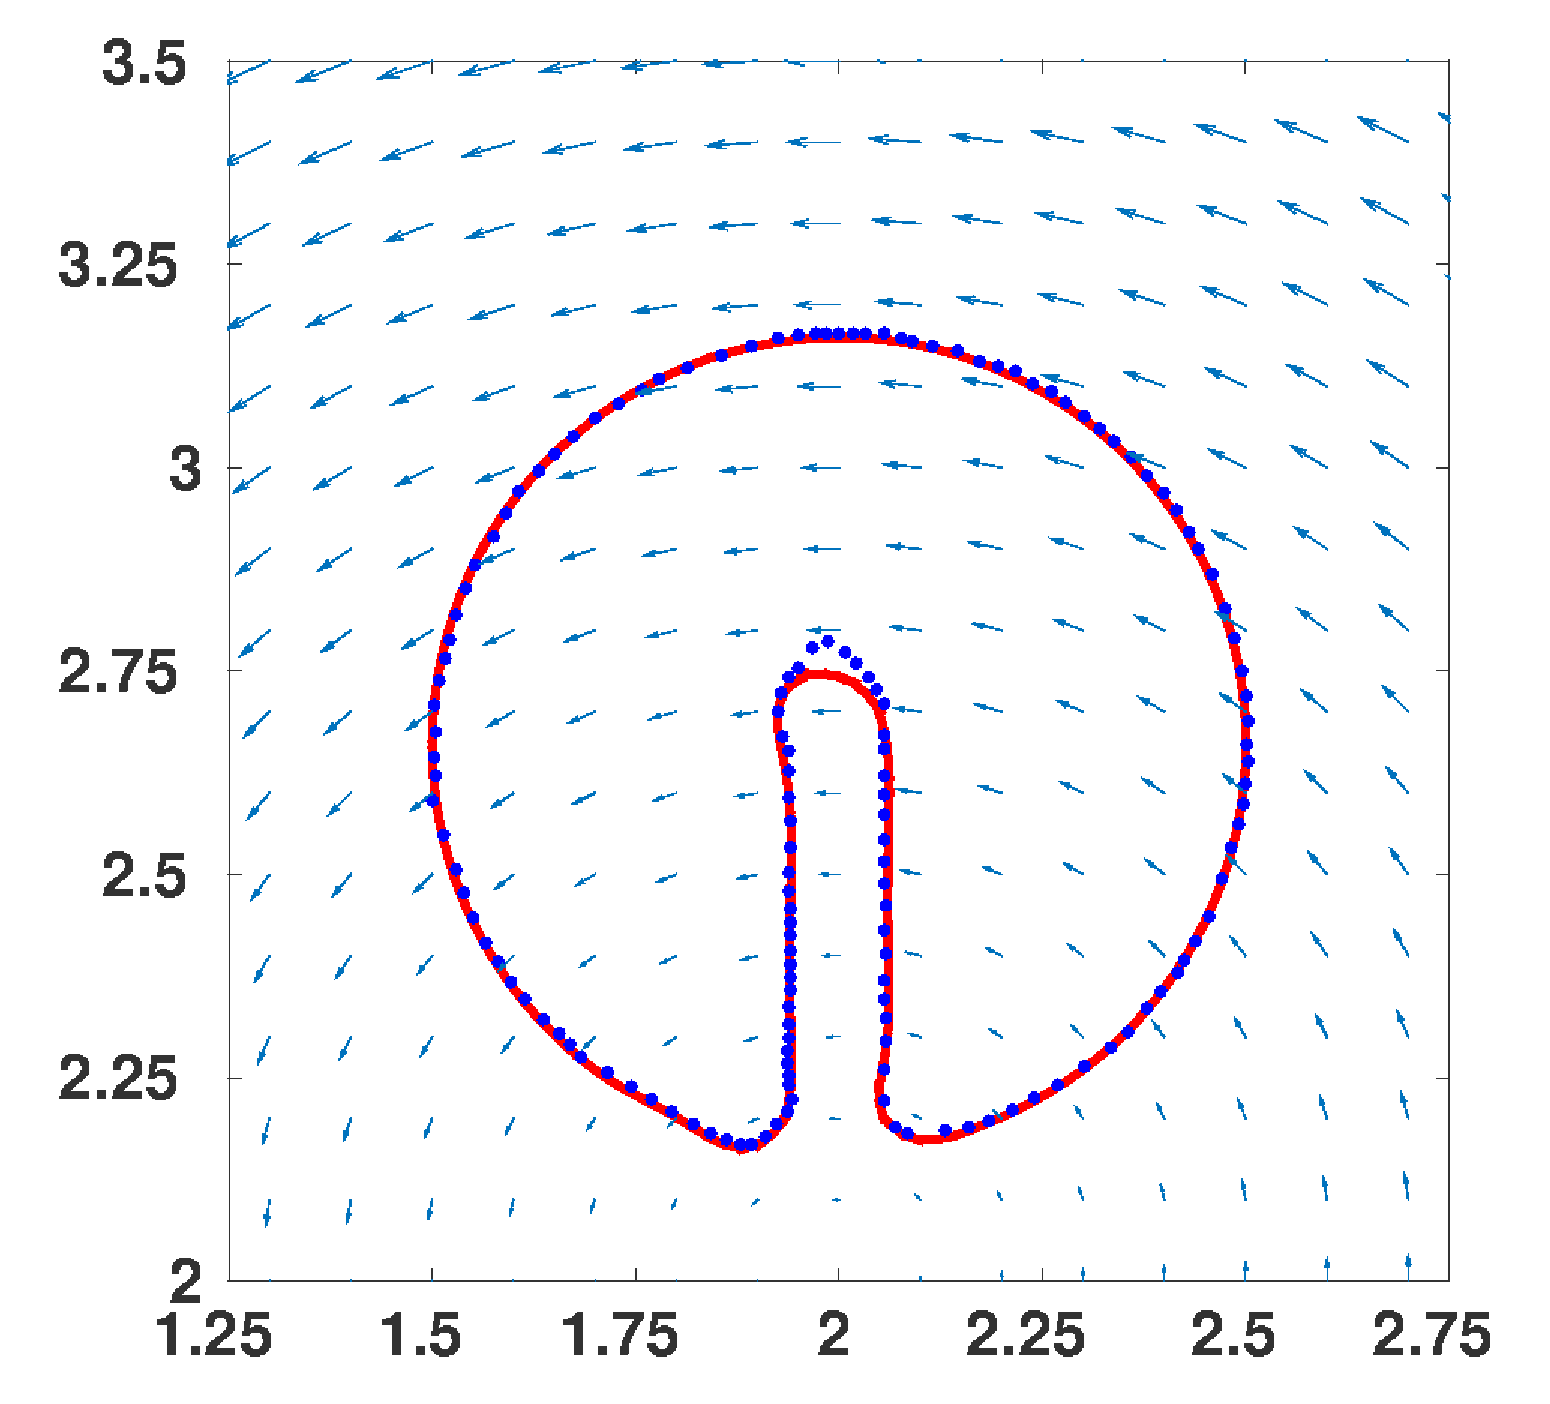
\includegraphics[width=0.5\textwidth]{SC_2513O.eps}
      }
 \caption{Comparison with \cite{Rudman1997} results. (Red LVIRA and Blue \cite{Rudman1997} data)}
 \label{Fig:rotation}
\end{figure}

\subsection{Shear Test}
The real problems typically encounters the interface deformation, which includes merging and deformation. Hence the algorithm has to be 
tested for shear velocity field (Figure \ref{Fig:shear}). The shear test problem verified with \cite{Gerlach2006}. (Figure \ref{Fig:shear_comparison}) 

   \begin{enumerate}
 \item Domain: [0,$\pi$] x [0,$\pi$]
 \item Grid Size: 100 x 100
 \item Radius of circle :$\frac{\pi}{5}$
 \item Center : $(\pi/2,\pi/4)$
 \item Velocity field(Forward):  $u=sin x cos y, v=-cos x sin y$
  \item Velocity field(Backward):  $u=-sin x cos y,v=cos x sin y$
 \end{enumerate}
 
\begin{figure}
\centering
   \subfloat[Initial condition for shear test ]{%
      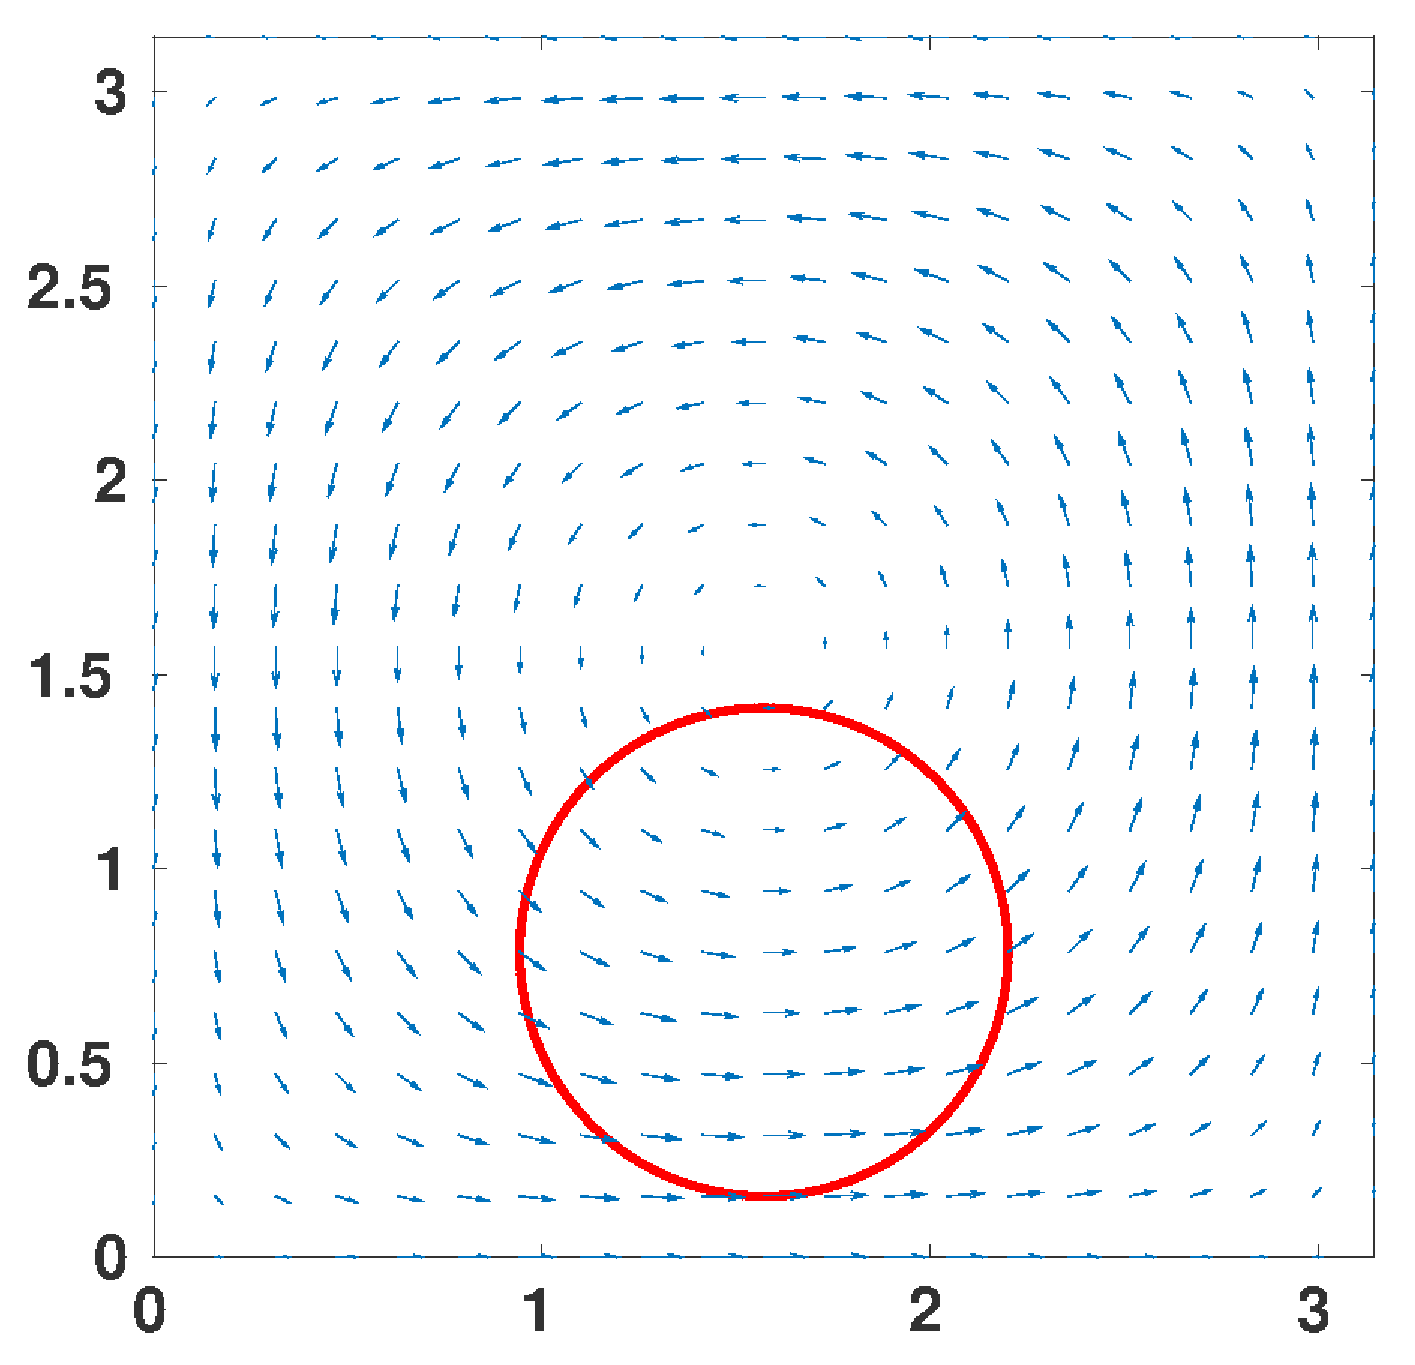
\includegraphics[width=0.5\textwidth]{shear_IC.eps}
      }
\subfloat[After advecting 250 steps ]{%
      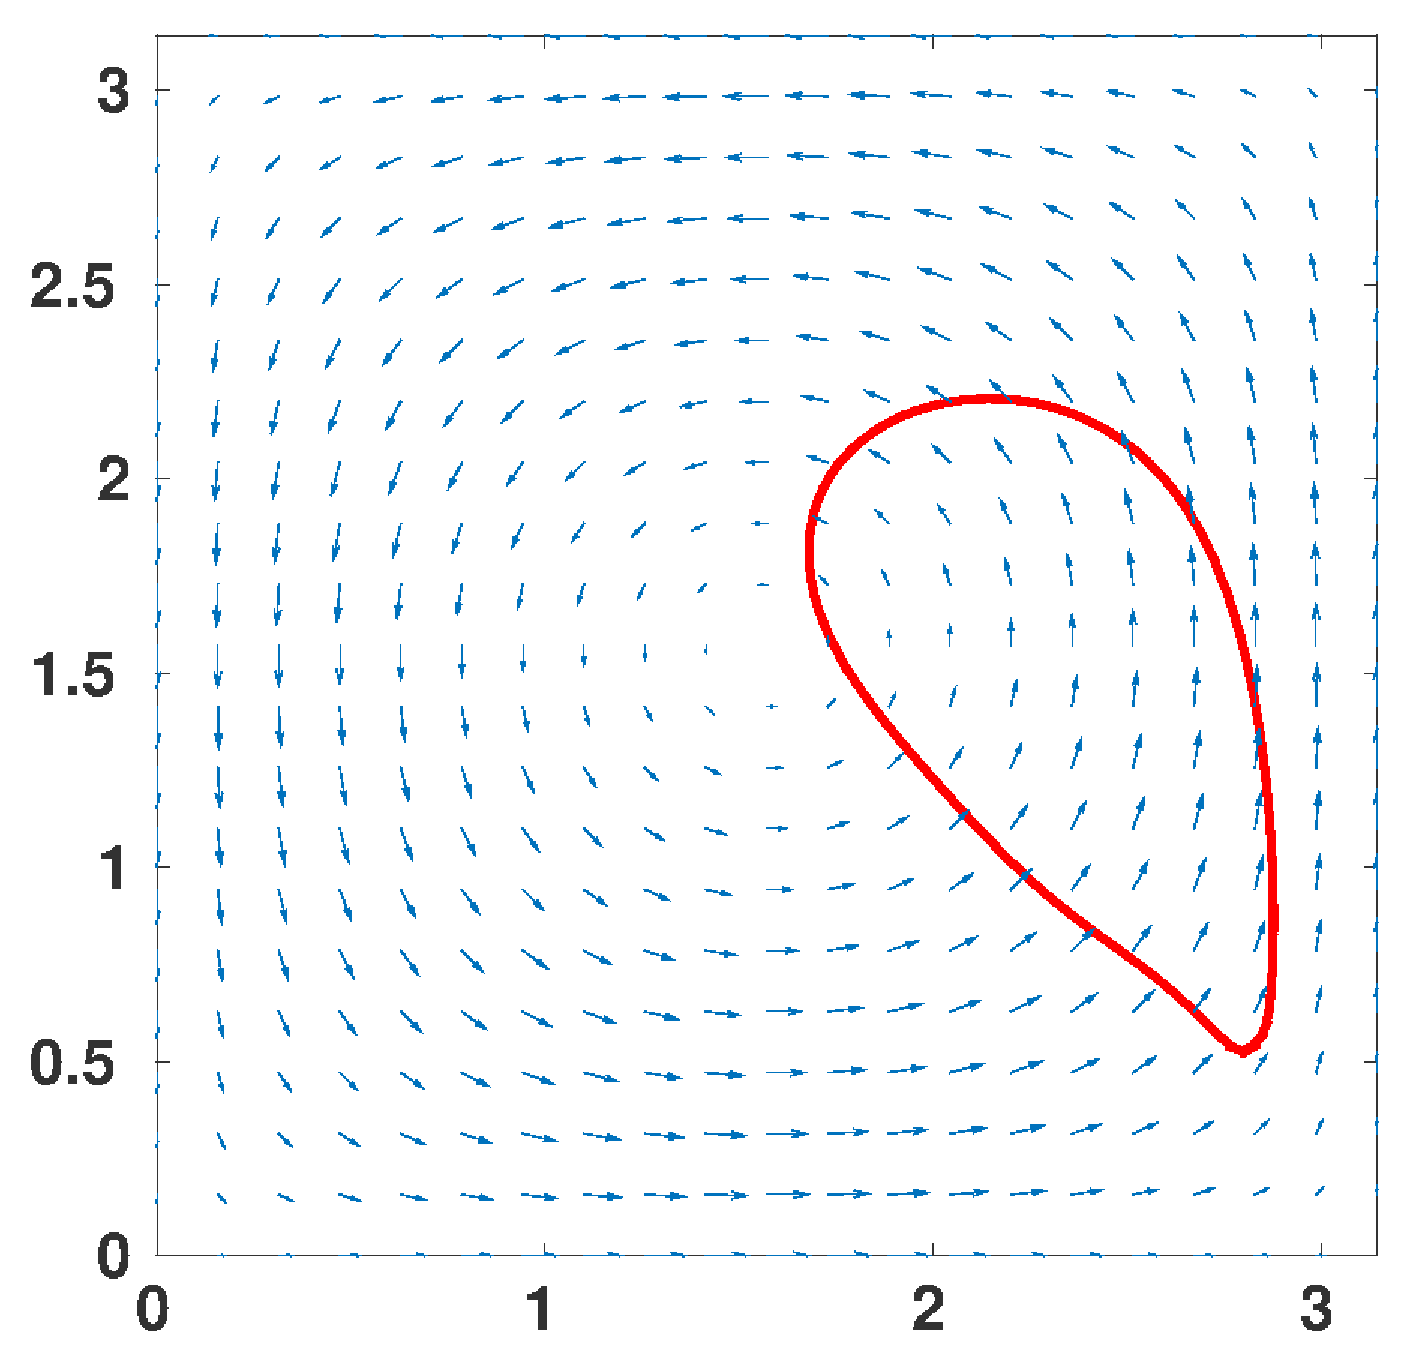
\includegraphics[width=0.5\textwidth]{shear_250.eps}
      } \\
      \subfloat[After advecting 500 steps ]{%
      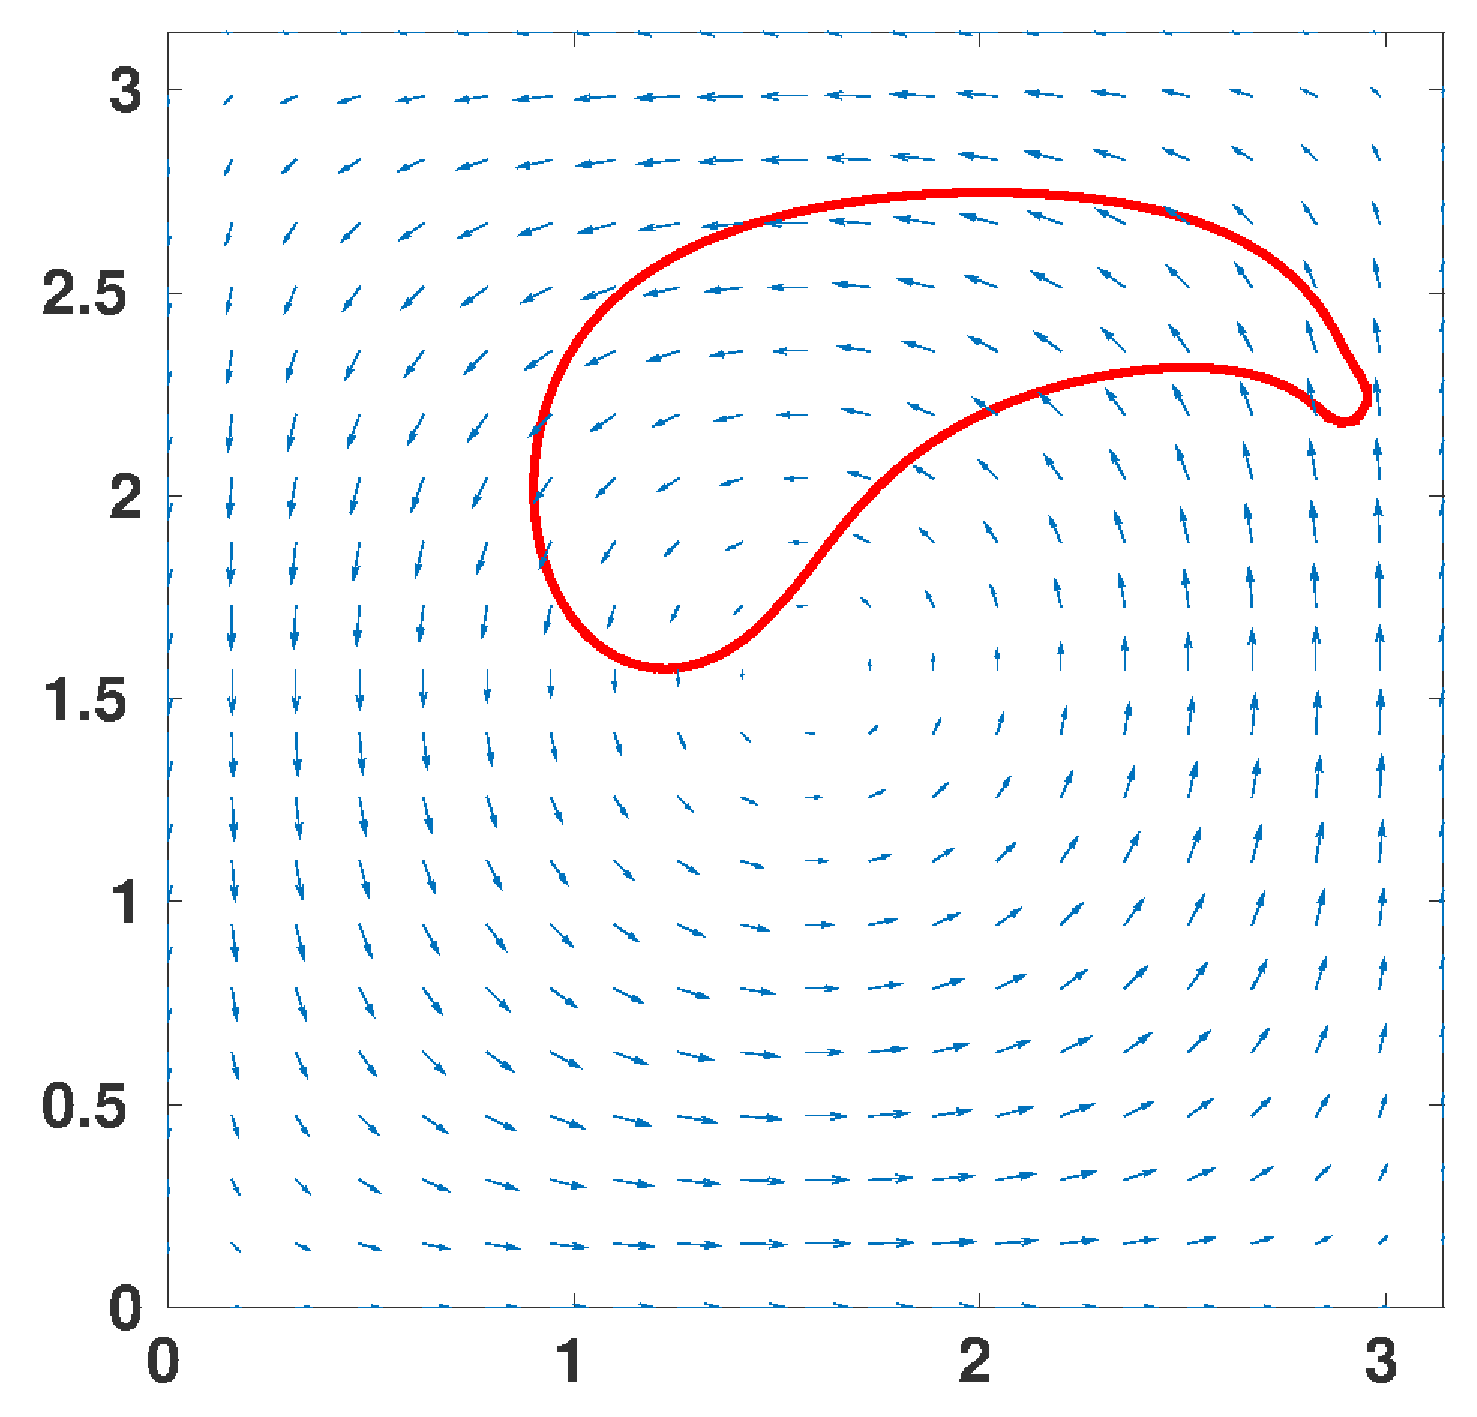
\includegraphics[width=0.5\textwidth]{shear_500.eps}
      }
      \subfloat[After advecting 1000 steps ]{%
      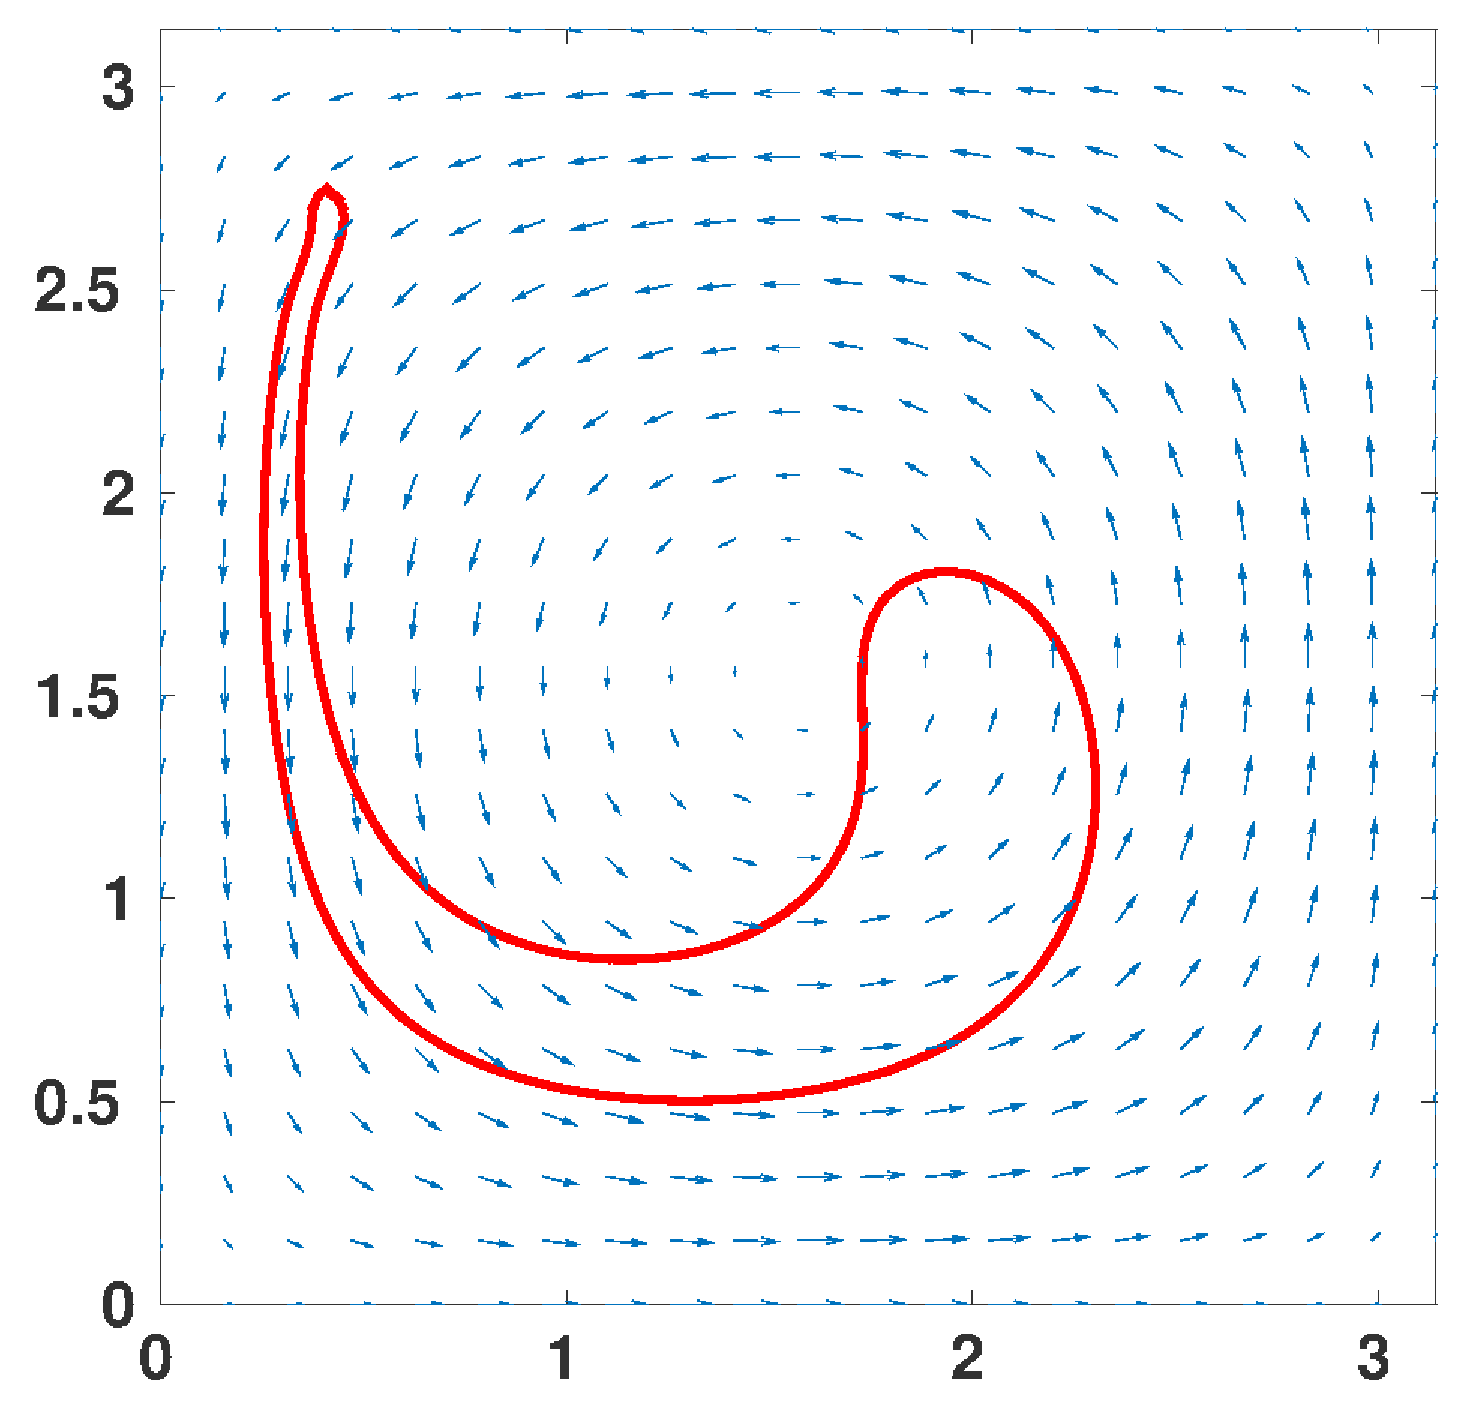
\includegraphics[width=0.5\textwidth]{shear_1000.eps}
      }
 \caption{Advection test result for shear velocity field}
 \label{Fig:shear}
\end{figure}

\begin{figure}
 \centering
 \subfloat[After 1000 steps forward ]{%
      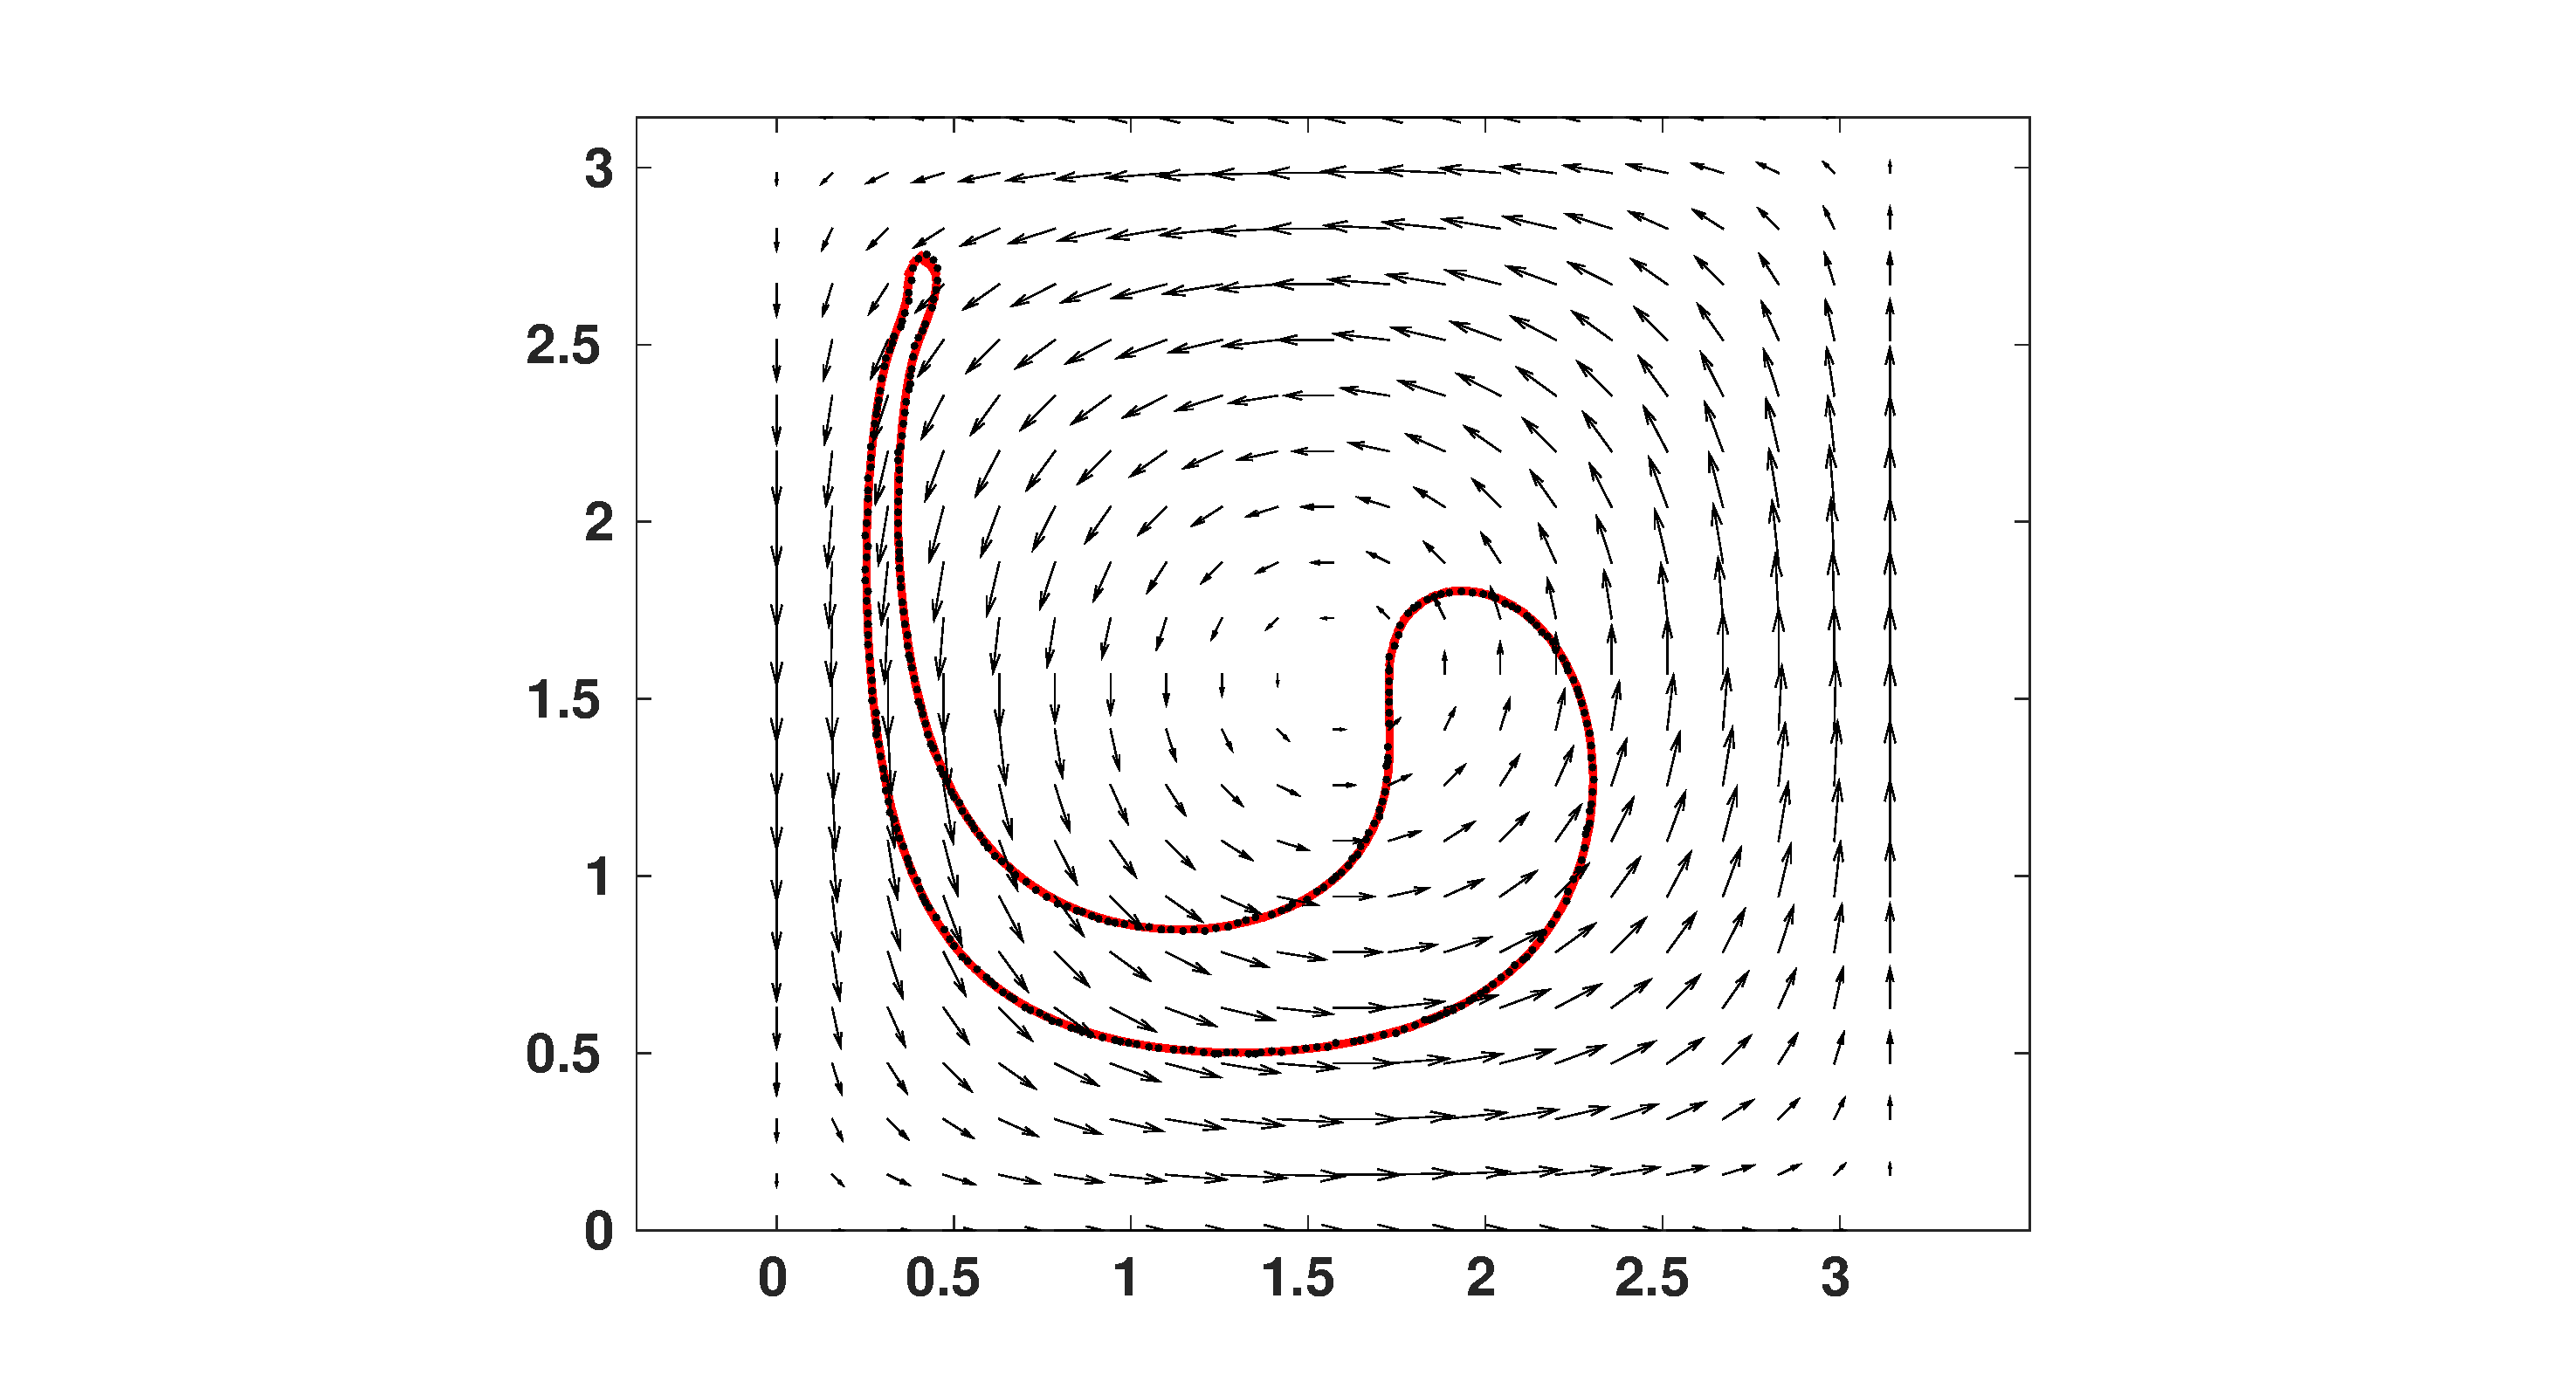
\includegraphics[width=0.5\textwidth]{shear_1000c.eps}
      }
  \subfloat[1000 steps backward followed by 1000 steps forward ]{%
      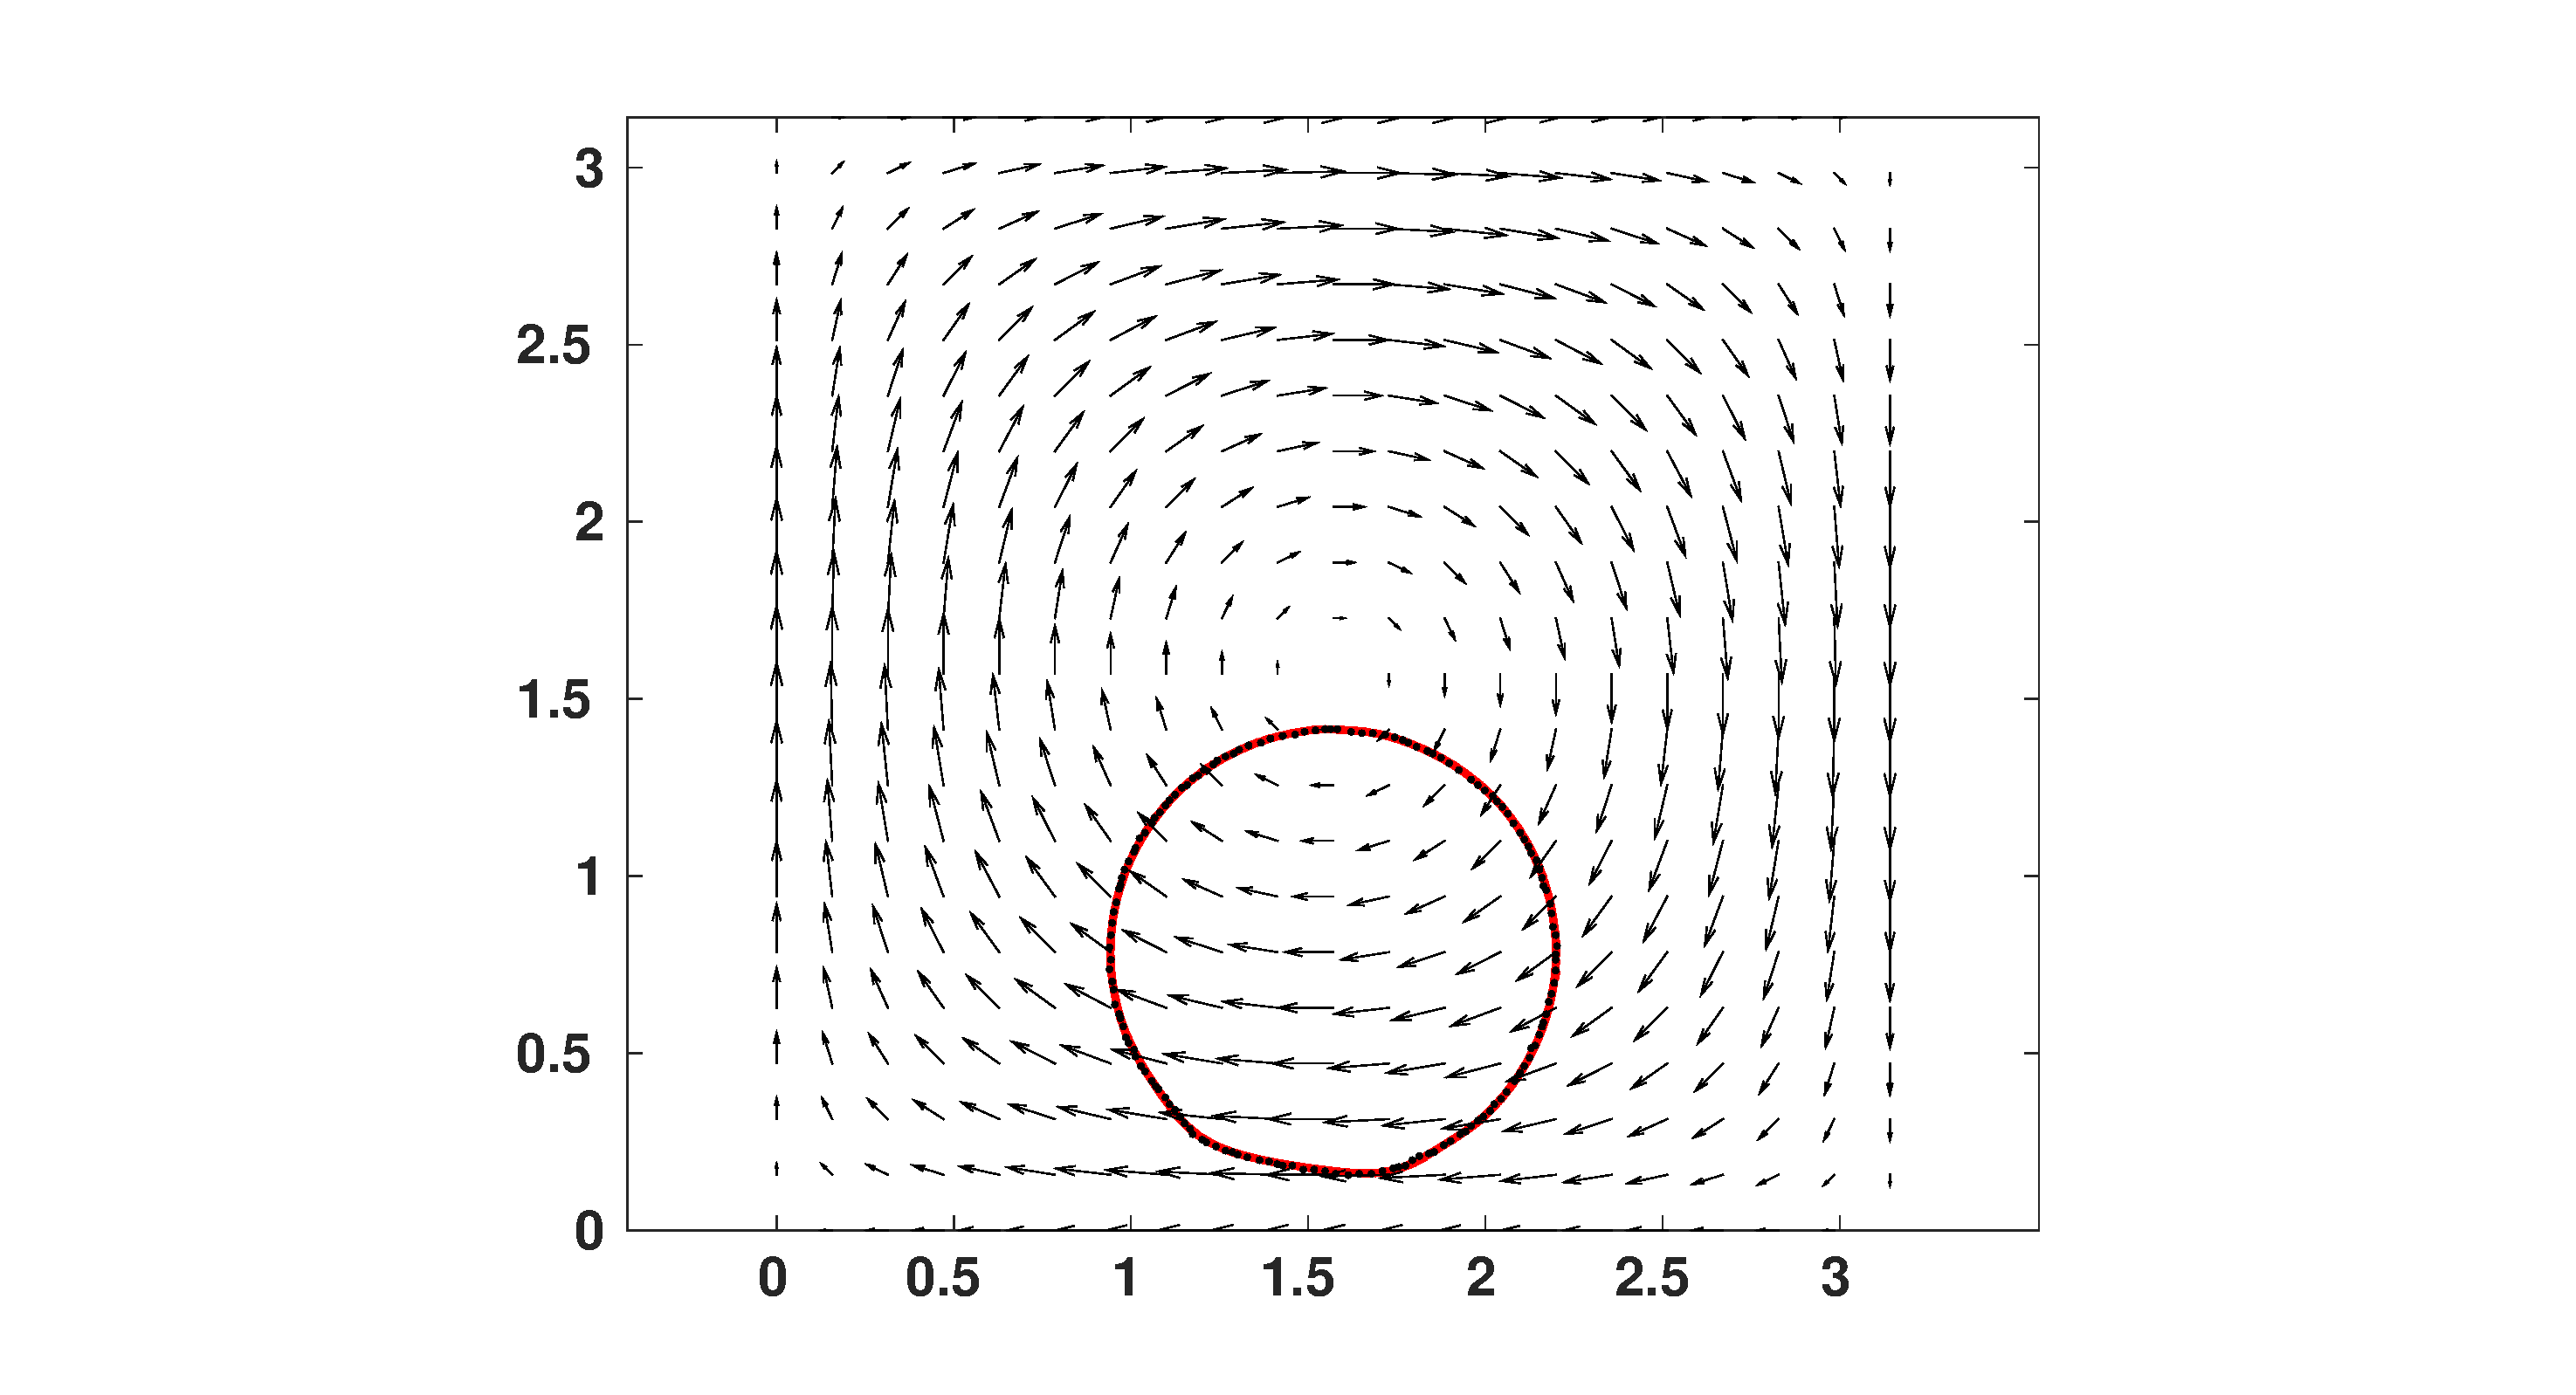
\includegraphics[width=0.5\textwidth]{shear_back.eps}
      }
 \caption{Comparison with \cite{Gerlach2006} results. (Red LVIRA and Blue \cite{Gerlach2006} data)}
 \label{Fig:shear_comparison}
\end{figure}

\subsection{Calculation of error}

The above results can be quantified by defining the error as
\begin{equation}
 E = \frac{\sum |{F^n_{r,c}-F^e_{r,c}}|}{\sum F^0_{r,c}}
\end{equation}
where E is the ratio of summation of difference between the volume fraction of cells of calculated solution and exact solution to the total sum inital volume fraction over all the cells.
where $F^n$ is the solution of volume fraction field after n time steps of computation, $F^e$ is the exact solution, and $F^0$ is the initial solution. The initial solution can be calculated by the initial 
volume fraction field, exact solution of field for translational velocity fields can be easily calculated by recreating the circle at the center which has moved with the velocity field. For solid body
rotation the exact solution is equal to the initial solution after one full rotation. For the shear test after 1000 backward steps the final solution should also be equal to initial solution.
The errors calculated for various tests are shown in Table \ref{Table:errors} and compared with \cite{Rudman1997}.

\begin{table}
  \begin{center}
    \caption{Errors for various tests}
 \label{Table:errors}
    \begin{tabular}{p{3cm}llll|a}
      \toprule 
       Test & SLIC & Hirt-Nichols & FCT-VOF & Youngs & LVIRA (Present Study)  \\ 
      \midrule
      Translational (V(1,0)) & $1.30 X 10^{-2}$ & $4.55 X 10^{-2}$ & $1.28 X 10^{-2}$ & $3.08 X 10^{-3}$ & $1.5 X 10^{-3}$  \\ 
        Translational (V(2,1)) & $9.18 X 10^{-2}$ & $1.9 X 10^{-1}$ & $3.99 X 10^{-2}$ & $2.98 X 10^{-2}$ & $1.05 X 10^{-2}$  \\ 
      Shear Flow & $4.59 X 10^{-2}$ & $6.66 X 10^{-2}$ & $3.14 X 10^{-2}$ & $8.60 X 10^{-3}$ & $6.90 X 10^{-3}$  \\ 
       Solid Body Rotation (Slotted circle) & $8.38 X 10^{-2}$ & $9.62 X 10^{-2}$ & $3.29 X 10^{-2}$ & $1.09 X 10^{-2}$ & $9.7 X 10^{-3}$  \\ 
        
      \bottomrule \\
    \end{tabular}
  \end{center}
\end{table}


\section{Conclusion}
The reconstruction and advection of an interface is calculated mostly geometrical techniques and does not require extensive knowledge of computational techniques. We found LVIRA
is more accurate than other methods available in the literature. We will couple this algorithm with a flow solver which we have discussed in the next chapter. 
 % \documentclass[a4paper,10pt]{report}
% \usepackage[utf8]{inputenc}
% \usepackage{amsmath}
% \usepackage{mathtools}
% \usepackage{graphicx}
% \usepackage{booktabs}
% \usepackage{caption}
% \usepackage{subcaption}
% \usepackage{float}
% \graphicspath{{images/}}
% 
% % Title Page
% \title{Navier Stokes Solver for two phase flow}
% \author{Palas Kumar farsoiya}

% 
% \begin{document}
% \maketitle
\chapter{Navier Stokes Solver for two phase flow}
% \begin{abstract}
% 
% \end{abstract}
\section{Governing Equations}
As we adopt continuum hypothesis, we then apply conservation principles to obtain governing equations for 
the fluid flow. These are conservation of mass, momentum and energy which are briefly described here. This derivation
is mostly adapted from \cite{Leal2007}.

\subsection{Mass conservation}
Consider a material volume element in Fig \ref{Fig:control_v}.  A material volume is one whose shape at time $t=0$, is arbitrary,
and has a fixed set of material points. And therefore, moves with the local continuum velocity of the fluid 
at every point.

\begin{wrapfigure}{r}{0.5\textwidth}
  \begin{center}
    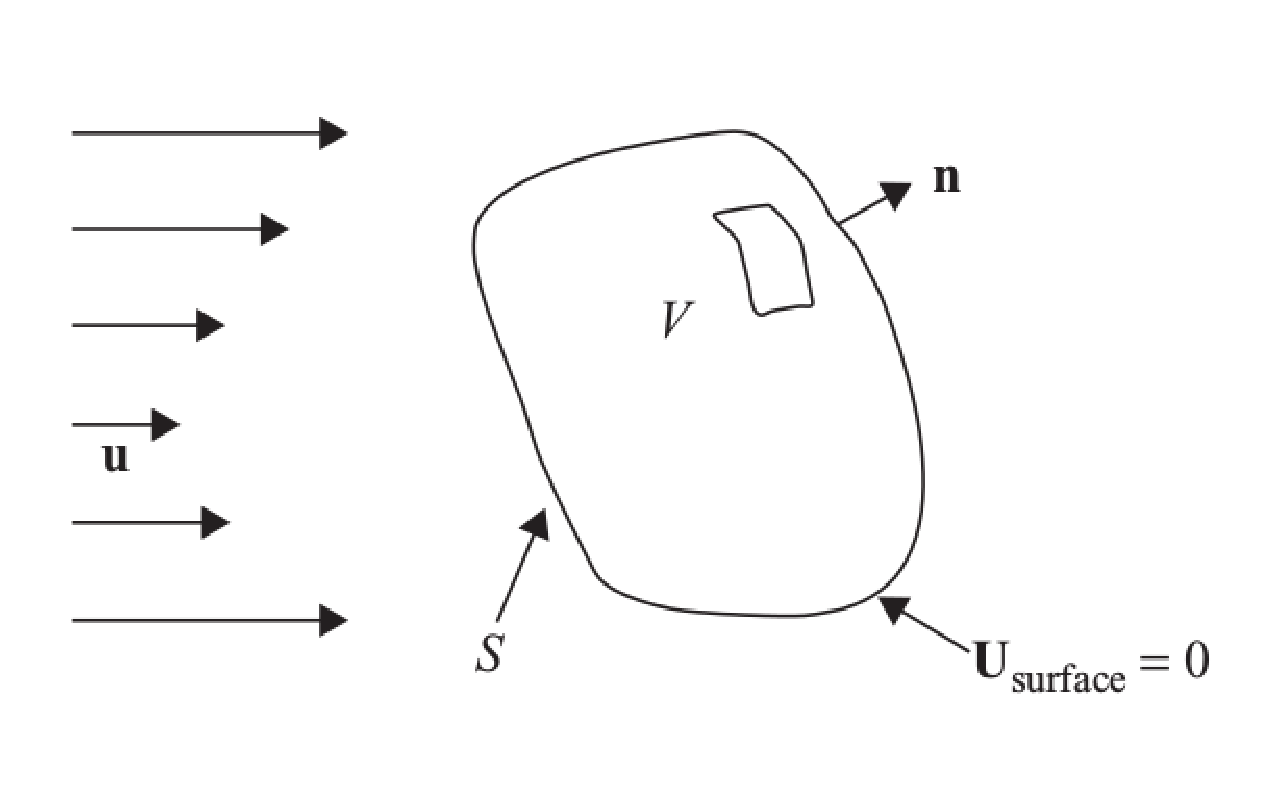
\includegraphics[width=0.48\textwidth]{control_v.eps}
  \end{center}
  \caption{An arbitrary control volume \cite{Leal2007}}
  \label{Fig:control_v}
\end{wrapfigure}

Conservation of mass states that mass is neither created nor destroyed. It implies that the mass inside the material volume is constant with respect
to time. Mathematically,
\begin{equation}
 \frac{D}{Dt}\left[\int_{V_m(t)}{\rho dV}\right] = 0 
 \label{Eq:1}
\end{equation}

where,
\begin{equation}
 \frac{DB}{Dt} = \frac{\partial B}{\partial t}+u.\nabla B
\end{equation}
Using the Reynolds transport theorem, which says

\begin{equation}
 \frac{D}{Dt}\left[\int_{V_m(t)}{}{B(x,t)}dV\right] = \int_{V_m(t)}{}{\left[\frac{\partial B}{\partial t} + \nabla . (Bu)\right] dV}
 \label{Eq:3}
\end{equation}

\ref{Eq:1}, can be written as, 
\begin{equation}
 \int_{V_m(t)}{}{\left[\frac{\partial \rho}{\partial t} + \nabla . (\rho u)\right] dV} = 0
\end{equation}

where the choice of $V_m(t)$ is arbitrary, hence the integrand itself must be zero.
\begin{equation}
 \frac{\partial \rho}{\partial t} + \nabla . (\rho u) = 0
 \label{Eq:5}
\end{equation}

For, incompressible fluids where density does not changes with time, \ref{Eq:5} reduces to,
\begin{equation}
 \nabla .u = 0
 \label{Eq:6}
\end{equation}

\subsection{Momentum Conservation}
Newton's second law states that,

\begin{equation}
 \textbf{Rate of change of linear momentum in an inertial frame} = \textbf{The sum of forces acting on the body}
\end{equation}

When we apply this to a material control volume, we obtain
\begin{equation}
 \frac{D}{Dt}\int_{V_m(t)} (\rho u) d V = \text{ sum of the forces acting on } V_m(t)
 \label{Eq:8}
\end{equation}

From a continuum perspective, the forces which act on the control volume can be of two types. Body force and surface force. The body force
which is common to most of the problems is gravitational force, which acts equally on all the volume elements. The surface forces are forces
are short range forces which acts on the surface of the control volume.

RHS of \ref{Eq:8}, can be expressed as sum of these two forces,
\begin{equation}
 \frac{D}{Dt}\int_{V_m(t)} (\rho u) d V = \int_{V_m(t)}{\rho g dV} + \int_{A_m(t)}{JdA}
 \label{Eq:9}
\end{equation}

where, g is acceleration due to gravity, $A_m(t)$ is the closed surface area of the control volume element and $J$ is the \textbf{stress vector}.
Using \ref{Eq:3}, we can write the RHS of \ref{Eq:9} as,

\begin{equation}
 \int_{V_m(t)}{}{\left[\frac{\partial (\rho u)}{\partial t} + \nabla . (\rho uu)\right] dV} =  \int_{V_m(t)}{\rho g dV} + \int_{A_m(t)}{JdA}
 \label{Eq:10}
\end{equation}

In the above equation stress vector $J$, can be found by linear vector operation on unit normal to the surface at any given point. The linear vector operator
is \textbf{T}, is called as stress tensor, which is a second order tensor. Thus, 

\begin{equation}
 J(n,x) = n . \textbf{T(x)} 
\end{equation}
Applying Gauss divergence theorem,
\begin{equation}
 \int_{A_m(t)}{n . \textbf{T}}dS  = \int_{V_m(t)}{\nabla . \textbf{T}} dV
\end{equation}
and substituting in \ref{Eq:10}, we get
\begin{equation}
 \int_{V_m(t)}{}{\left[\frac{\partial (\rho u)}{\partial t} + \nabla . (\rho uu)\right] dV} =  \int_{V_m(t)}{\rho g dV} + \int_{V_m(t)}{\nabla . \textbf{T}}
\end{equation}

After rearrangement, 
\begin{equation}
 \int_{V_m(t)}{\left[\frac{\partial (\rho u)}{\partial t} + \nabla . (\rho uu)  -  \rho g  - \nabla . \textbf{T}\right]dV} = 0
\end{equation}

Again, the $V_m(t)$, is an arbitrary control volume, and the integrand must be then zero. Thus we obtain,

\begin{equation}
 \frac{\partial (\rho u)}{\partial t} + \nabla . (\rho uu)  =  \rho g  + \nabla . \textbf{T} 
 \label{Eq:15}
\end{equation}

The stress tensor \textbf{T} can be expressed in terms of isotropic and non-isotropic parts,

\begin{equation}
 \textbf{T} = -p\textbf{I}+\textbf{$\tau$ }
\end{equation}
Substitute this form in \ref{Eq:15}, we get

\begin{equation}
 \frac{\partial (\rho u)}{\partial t} + \nabla . (\rho uu)  = \nabla .( -p\textbf{I}+\tau) + \rho g  
 \label{Eq:17}
\end{equation}
The constitutive equation for a Newtonian fluid is,
\begin{equation}
 \textbf{$\tau$} = 2\mu \textbf{D}
 \label{Eq:18}
\end{equation}
where, \textbf{$D$} is the rate of strain tensor, the symmetric part of $\nabla u$. Now,
\begin{equation}
 \text{$\tau$} = \mu (\nabla u + (\nabla u)^T)
 \label{Eq:19}
\end{equation}

Substituting this in \ref{Eq:17}, we get
\begin{equation}
 \frac{\partial (\rho u)}{\partial t} + \nabla . (\rho uu)  =  -\nabla p+ \nabla .(\mu (\nabla u + (\nabla u)^T)) + \rho g  
 \label{Eq:20}
\end{equation}
Subtracting \ref{Eq:5} from \ref{Eq:20}, we get
\begin{equation}
 \frac{\partial u}{\partial t} + (u.\nabla)u  =  -\frac{\nabla p}{\rho}+ \frac{1}{\rho}\nabla .(\mu (\nabla u + (\nabla u)^T)) +  g   
 \label{Eq:21}
\end{equation}
Rewriting \ref{Eq:21}, in conservative form, using mass conservation
\begin{equation}
 \frac{\partial u}{\partial t} + \nabla .(uu)  =  -\frac{\nabla p}{\rho}+ \frac{1}{\rho}\nabla .(\mu (\nabla u + (\nabla u)^T)) +  g  
 \label{Eq:22}
\end{equation}

\subsection{Non-Dimensionalisation of governing equations}
For non-dimensionalisation we chose scale as characteristic length  L, characteristic velocity U, characteristic time $\frac{L}{U}$, characteristic pressure $\rho_L U^2$,
characteristic density $\rho_L$ and characteristic viscosity $\mu_L$.
Substitute $u = U\tilde u $, $x = L\tilde x $, $y = L\tilde y $, $t = \frac{L}{U}\tilde t $, $p = \rho_L U^2\tilde p $, $\rho = \rho_L \tilde\rho $, $\mu = \mu_L \tilde\mu $
in \ref{Eq:22}, where quantities with tilde are non-dimensional.

\begin{equation}
 \frac{U^2}{L}\left[\frac{\partial \tilde u}{\partial \tilde t} + \tilde\nabla .(\tilde u \tilde u)\right]  = -\frac{\rho_L}{\rho_L \tilde\rho}\frac{U^2}{L}\tilde\nabla \tilde p
 + \frac{U^2}{L^2\rho_L \tilde\rho}\tilde \nabla .(\mu_L \tilde\mu (\tilde\nabla \tilde u + (\tilde\nabla \tilde u)^T)) +  g 
 \label{Eq:23}
\end{equation}

Rearranging \ref{Eq:23},

\begin{equation}
 \left[\frac{\partial \tilde u}{\partial \tilde t} + \tilde\nabla .(\tilde u \tilde u)\right]  = -\frac{1}{\tilde\rho}\tilde\nabla \tilde p
 + \frac{\mu_L}{L\rho_L U}\frac{1}{\tilde\rho}\tilde \nabla .(\tilde\mu (\tilde\nabla \tilde u + (\tilde\nabla \tilde u)^T)) +  \frac{gL}{U^2} 
 \label{Eq:24}
\end{equation}

Now, dropping tilde from the quantities,
\begin{equation}
 \frac{\partial  u}{\partial  t} + \nabla .( u  u)  = -\frac{1}{\tilde\rho}\nabla  p
 + \frac{1}{Re_L}\frac{1}{\tilde\rho} \nabla .(\tilde\mu (\nabla  u + (\nabla  u)^T)) +  \frac{1}{Fr^2} 
 \label{Eq:25}
\end{equation}

where, $Re_L = \frac{L\rho_L U}{\mu_L}$, $We_L = \frac{L \rho_L U^2}{\sigma_{LG}}$ and $Fr = \frac{U}{\sqrt{gL}}$. 

\ref{Eq:25} is the non-dimensional form for incompressible multiphase newtonian flow.

\subsection{Integral form of governing equation}
As the conservation equations are valid for a differential element, we can also integrate them over a control volume. This is the final step before the finite volume discretisation
approach.\ref{Eq:25} can be integrated on a control volume, V 

\begin{equation}
\int_V\left[ \frac{\partial  u}{\partial  t} + \nabla .( u  u)\right]dV  = \int_V\left[-\frac{1}{\tilde\rho}\nabla  p
 + \frac{1}{Re_L}\frac{1}{\tilde\rho} \nabla .(\tilde\mu (\nabla  u + (\nabla  u)^T)) +  \frac{1}{Fr^2}\right]dV 
 \label{Eq:26}
\end{equation}

\begin{equation}
\int_V \frac{\partial  u}{\partial  t}dV +\int_V \nabla .( u  u)dV  = -\int_V\frac{1}{\tilde\rho}\nabla  p dV
 + \frac{1}{Re_L}\frac{1}{\tilde\rho} \int_V\nabla .(\tilde\mu (\nabla  u + (\nabla  u)^T))dV +  \frac{1}{Fr^2}\int_V dV \nonumber \\
 \label{Eq:27}
\end{equation}
Applying Gauss divergence theorem on advection and diffusion intergrals, we get
\begin{equation}
\int_V \frac{\partial  u}{\partial  t}dV +\int_S u(u.n)dS  = -\int_V\frac{1}{\tilde\rho}\nabla  p dV
 + \frac{1}{Re_L}\frac{1}{\tilde\rho} \int_S (\tilde\mu (\nabla  u + (\nabla  u)^T).n)dS +  \frac{1}{Fr^2}\int_VdV \nonumber \\
 \label{Eq:28}
\end{equation}

Now, we can average the individual quantities over the control volume, V and Equation \ref{Eq:29} is used for discretisation in our code.
\begin{eqnarray}
\frac{1}{V}\int_V \frac{\partial  u}{\partial  t}dV +\frac{1}{V}\int_S u(u.n)dS  = -\frac{1}{V}\int_V\frac{1}{\tilde\rho}\nabla  p dV \nonumber
 + \frac{1}{Re_L}\frac{1}{\tilde\rho} \frac{1}{V}\int_S (\tilde\mu (\nabla  u + (\nabla  u)^T).n)dS \nonumber \\
 +  \frac{1}{Fr^2}\frac{1}{V}\int_VdV \nonumber \\
 \label{Eq:29}
\end{eqnarray}

\section{Discretisation of governing equations}
\subsection{Grid}
 \setlength\intextsep{0pt}
\begin{wrapfigure}{r}{0.4\textwidth}
  \begin{center}
    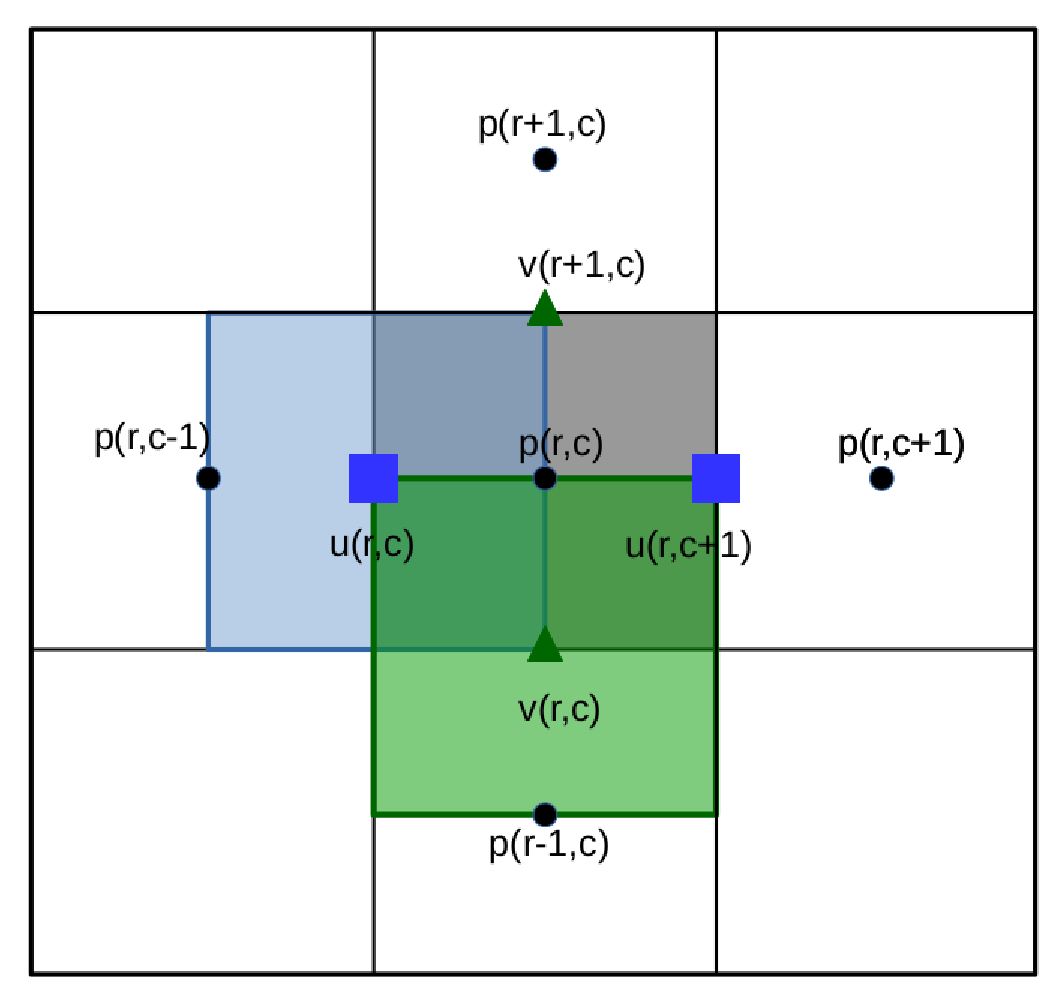
\includegraphics[width=0.4\textwidth]{grid_st.eps}
  \end{center}
  \caption{Staggered grid for x-velocity(Blue),y-velocity(Green) and pressure(Gray)}
  \label{Fig:grid_st}
\end{wrapfigure}
Before discretisation, we first specify our domain, grid shape and approach. The grid is rectangular and uniform grid spacing has been used for both x and y directions.
Figure \ref{Fig:grid_st} and \ref{Fig:grid} shows the grid and location of pressure and velocity nodes.
We can see the nodes of pressure and velocities are not colocated because decoupling of pressure and velocity may occur since the discretised form of equation of continuity 
on colocated grids can lead to checkerboard patterns in the solution(\cite{Anderson1995}). Staggered grid approach is used to avoid pressure-velocity decoupling. 
There are three different grids for x-velocity (u),y- velocity(v) and pressure (p).  
The momentum equation are discretised using finite volume approach using the conservative form of equations. This would first order in time and a predictor-corrector approach to 
compute velocity field in the domain.
 \begin{figure}
 \centering
  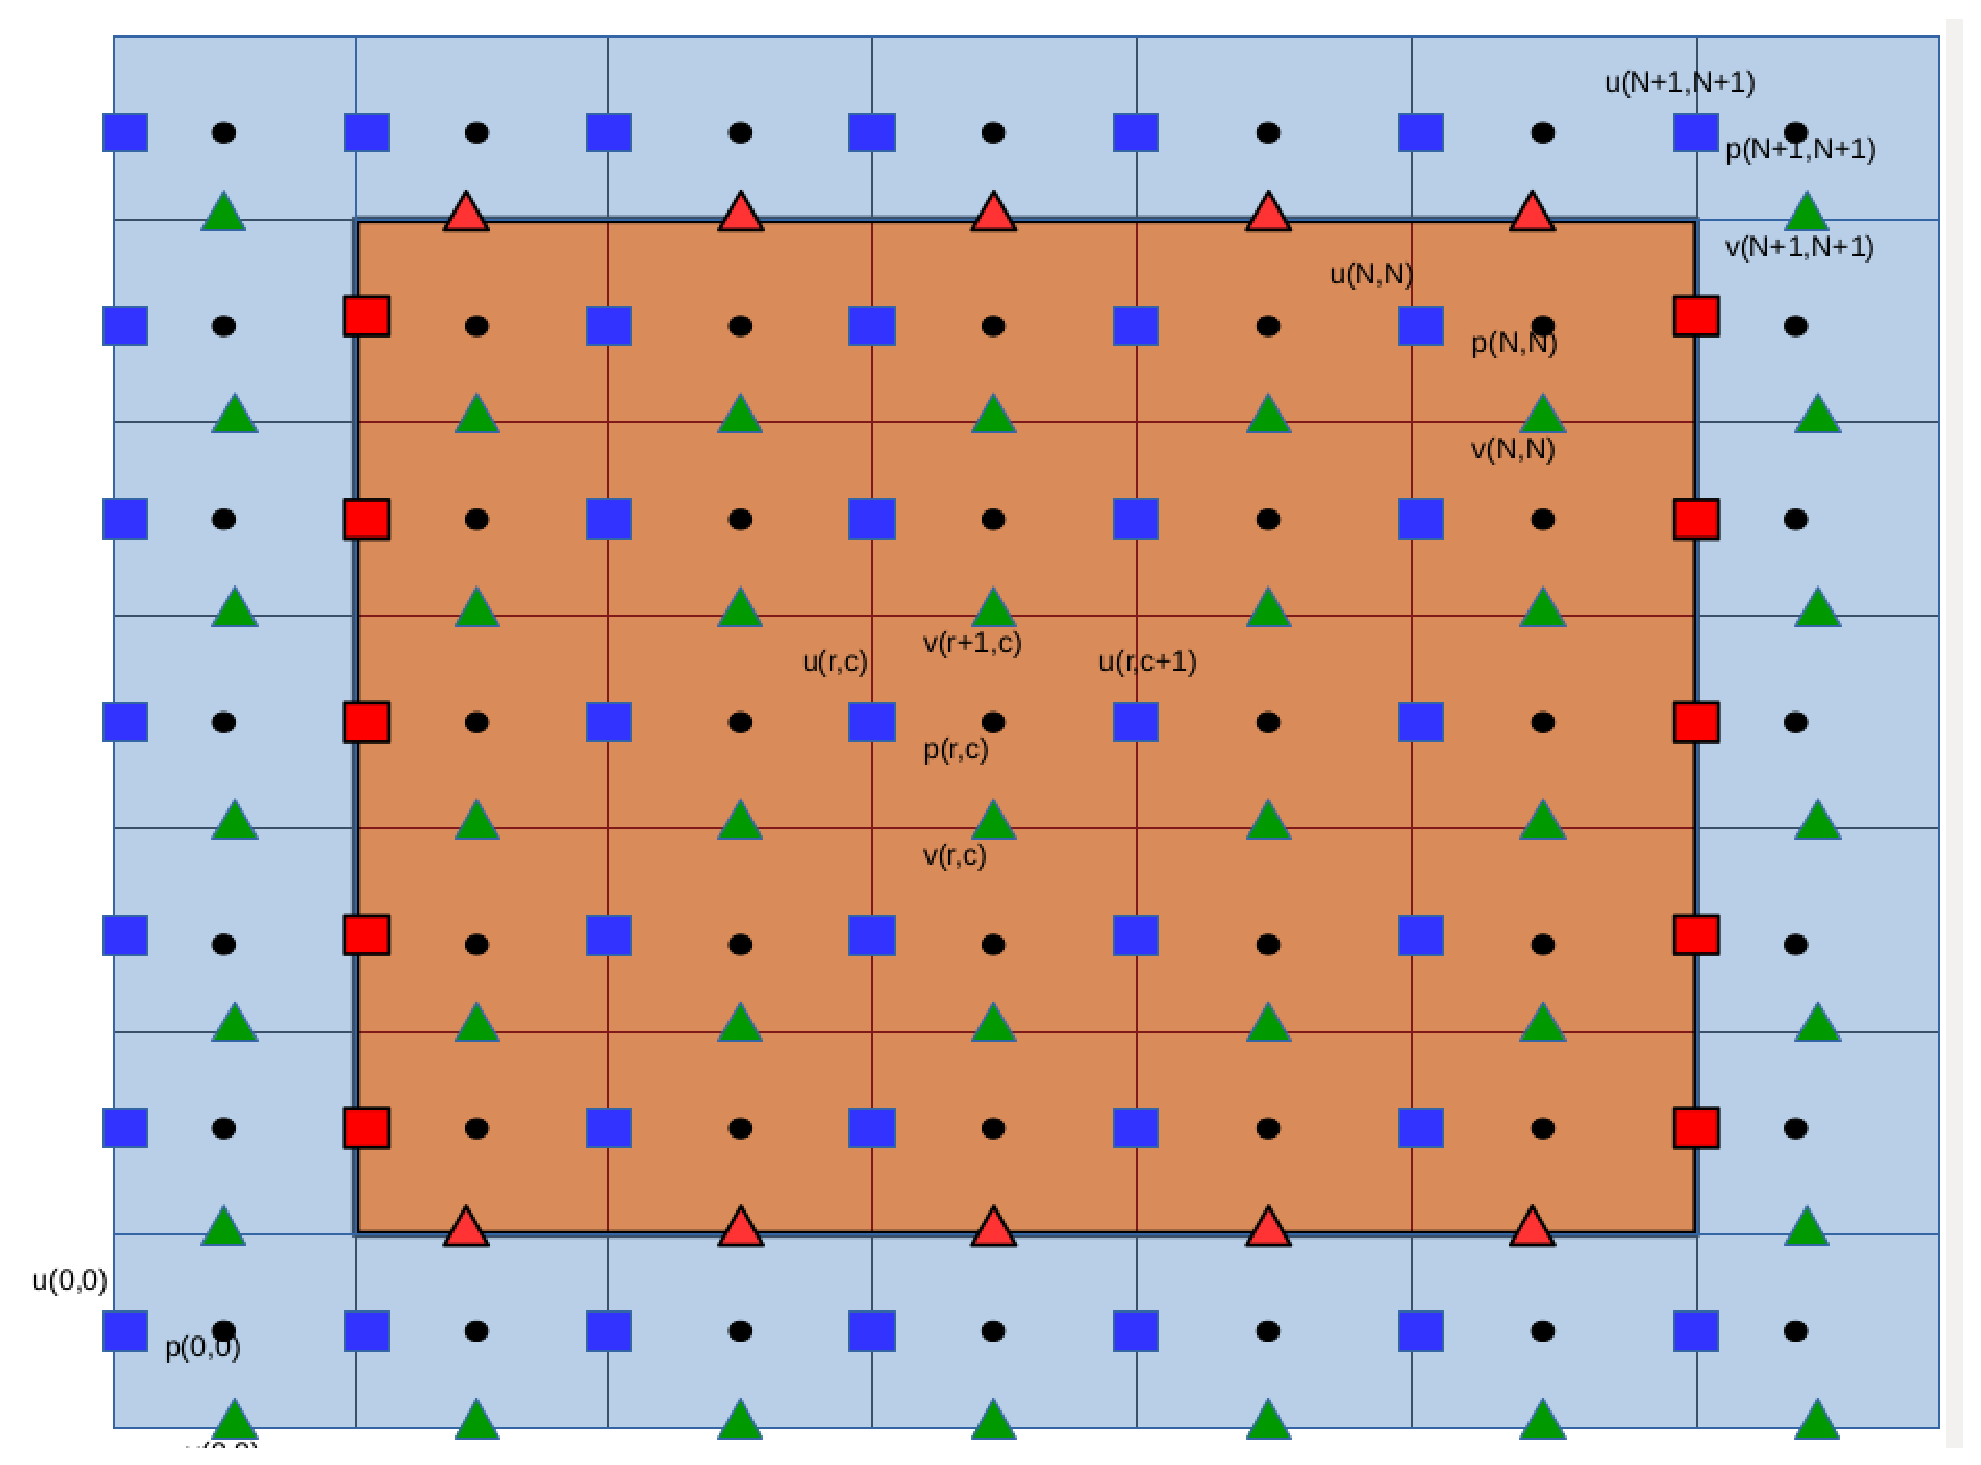
\includegraphics[scale=0.3]{pressure_calc.eps}
  \caption{Location of nodes, blue square:x-velocity, red square:boundary x-velocity, green triangle:y-velocity, red triangle:boundary y-velocity,black dot:pressure}
  \label{Fig:grid}
 \end{figure}


\subsection{Integration in time}
The first step is  to compute projected velocity, ignoring the pressure terms, 
\begin{equation}
 \frac{u^*-u^n}{\Delta t} =  -A^n + D^n + B^n
\end{equation}
where $u^n$ is the velocity at previous time step and $u^*$ is the projected velocity without taking pressure into consideration, 
where $A = \frac{1}{V}\int_S u(u.\hat{n})dS$ ,\\ \\ $D =\frac{1}{V}\frac{1}{Re_L}\frac{1}{\tilde\rho} \frac{1}{V}\int_S (\tilde\mu (\nabla  u + (\nabla  u)^T).\hat{n})dS $ and \\ \\
$B = \frac{1}{Fr^2}\frac{1}{V}\int_VdV  $
And then adding the pressure component in the projected velocity,

\begin{equation}
 \frac{u^{n+1}-u^*}{\Delta t} = -\frac{1}{V}\int_V\frac{1}{\rho}\nabla  p^{n+1} dV
\end{equation}

Rearranging,
\begin{equation}
 u^{n+1} = u^*-\frac{\Delta t}{V}\int_V\frac{1}{\rho}\nabla  p^{n+1} dV
\end{equation}

\subsection{Discretisation of advection terms}
To evaluate the advection terms, integrate it over the surface of the control volume. It is actually the sum of in and out fluxes through the faces of control volume. 
Here an approximation is made by assuming a uniform velocity on the faces of control volume and the fluxes are thus calculated by the value at the center of the boundary. 
Weighted Essentially Non-Oscillatory(WENO) [\cite{liu1994weighted}, \cite{jiang1995efficient}] scheme has been used to approximate the values of velocities at the face centers.
\begin{figure}
 \centering
 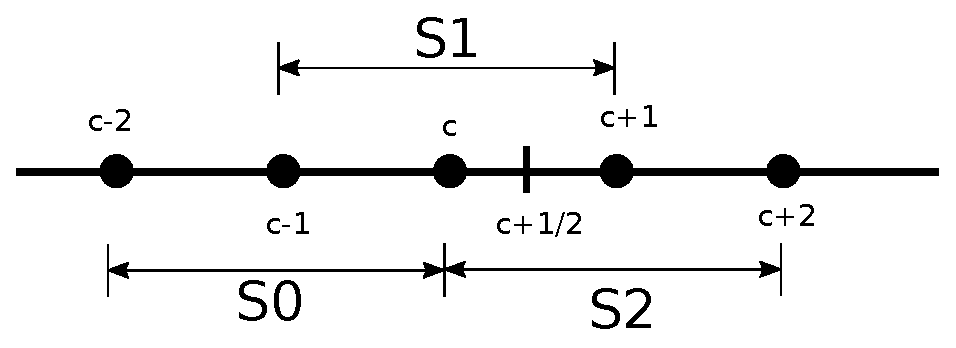
\includegraphics{wen_stencil.eps}
 \caption{Three sub stencils for reconstruction of $u_{i+1/_2}$}
\end{figure}

\begin{eqnarray*}
u^{(0)}_{c+1/_2} &=& \frac{1}{3}u_{c-2} - \frac{7}{6}u_{c-1} + \frac{11}{6} u_{c} \\
u^{(1)}_{c+1/_2} &=& -\frac{1}{6}u_{c-1} + \frac{5}{6}u_{c} + \frac{1}{3}u_{c+1} \\
u^{(2)}_{c+1/_2} &=& \frac{1}{3}u_{c} + \frac{5}{6}u_{c+1} − \frac{1}{6}u_{c+2} \\
\end{eqnarray*}

Once we get $u^{k}_{c+1/_2}$ from the three sub-stencils, we can get,
\begin{equation}
 u_{c+1/_2} = \sum_{k=0}^2 \omega_k u^{(k)}_{c+1/_2} %+ \omega_1 u^{(1)}_{c+1/_2} + \omega_2 u^{(2)}_{c+1/_2}
\end{equation}
where $\omega_k$ is given by,
\begin{eqnarray*}
 \omega_k = \frac{\tilde\omega_k}{\sum_{k=0}^2 \tilde\omega_k}, \qquad
 \tilde\omega_k = \frac{\gamma_k}{(\epsilon+\beta_k)^2} \\
 \gamma_0 = \frac{1}{10}, \quad \gamma_1 = \frac{3}{5}, \quad\text{and}\quad \gamma_2 = \frac{3}{10} \\
  \epsilon = 10^{-6}
\end{eqnarray*}
And, smoothness indicator $\beta_k$ is given by,
\begin{eqnarray*}
\beta_0 &=& \frac{13}{12}(u_{c-2} - 2u_{c-1} + u_c)^2 + \frac{1}{4}(u_{c-2}-4u_{c-1}+3u_c)^2\\
\beta_1 &=& \frac{13}{12}(u_{c-1} - 2u_{c} + u_{c+1})^2 + \frac{1}{4}(u_{c-1}-u_{c+1})^2\\
 \beta_2 &=& \frac{13}{12}(u_{c} - 2u_{c+1} + u_{c+2})^2 + \frac{1}{4}(3u_{c}-4u_{c+1}+u_{c+2})^2\\
\end{eqnarray*}

\begin{eqnarray}
 (A_x)_{net} &=& \frac{1}{V}\int_S u(u.n)dS \\
	 &=& \frac{1}{\Delta x \Delta y}\left[\int_{right} u(u.n)ds - \int_{left} u(u.n)ds + \int_{top} u(u.n)ds - \int_{bottom} u(u.n)ds\right] \nonumber \\
 \end{eqnarray}
% \begin{eqnarray*}
% \int_{right} u(u.n)ds &=& \left[\left(\frac{u_{r,c+1}+u_{r,c}}{2}\right)^2\right]\Delta y \\
% \int_{left} u(u.n)ds &=& \left[\left(\frac{u_{r,c}+u_{r,c-1}}{2}\right)^2\right]\Delta y \\
% \int_{top} u(u.n)ds &=& \left[\left(\frac{v_{r+1,c}+v_{r+1,c-1}}{2}\right)\left(\frac{u_{r+1,c}+u_{r,c}}{2}\right)\right]\Delta x \\
% \int_{top} u(u.n)ds &=& \left[\left(\frac{v_{r,c}+v_{r,c-1}}{2}\right)\left(\frac{u_{r,c}+u_{r-1,c}}{2}\right)\right]\Delta x \\
% \end{eqnarray*}
% Now, $(A_x)_{net}$ is now given by,
%  \begin{eqnarray*}
%  (A_x)_{net} =  \frac{1}{\Delta x}\left[\left(\frac{u_{r,c+1}+u_{r,c}}{2}\right)^2-\left(\frac{u_{r,c}+u_{r,c-1}}{2}\right)^2\right] \\
%  + \frac{1}{\Delta y}\left[\left(\frac{v_{r+1,c}+v_{r+1,c-1}}{2}\right)\left(\frac{u_{r+1,c}+u_{r,c}}{2}\right) 
%  -\left(\frac{v_{r,c}+v_{r,c-1}}{2}\right)\left(\frac{u_{r,c}+u_{r-1,c}}{2}\right)\right]
%  \end{eqnarray*}
% Similarly, $(A_y)_{net}$ is,
%   \begin{eqnarray*}
%  (A_y)_{net} =   \frac{1}{\Delta x}\left[\left(\frac{v_{r,c+1}+v_{r,c}}{2}\right)\left(\frac{u_{r,c+1}+u_{r-1,c+1}}{2}\right) 
%  -\left(\frac{v_{r,c}+v_{r,c-1}}{2}\right)\left(\frac{u_{r,c}+u_{r-1,c}}{2}\right)\right] \\
%  +\frac{1}{\Delta y}\left[\left(\frac{v_{r,c+1}+v_{r,c}}{2}\right)^2-\left(\frac{v_{r,c}+v_{r,c-1}}{2}\right)^2\right]
%  \end{eqnarray*}
 
 \subsection{Diffusion terms}
 Before looking at the discretised form of diffusion terms, we shall derive the components for x and y directions.
 
\subsubsection{Components of Diffusion term}
Gradient of velocity for 2D flow, 
\begin{equation*}
 \nabla u =  \begin{bmatrix} \frac{\partial u}{\partial x} & \frac{\partial u}{\partial y} \\ \frac{\partial v}{\partial x} & \frac{\partial v}{\partial y}  \end{bmatrix}
\end{equation*}

\begin{equation*}
 \nabla u + (\nabla u)^T=  \begin{bmatrix} \frac{\partial u}{\partial x} & \frac{\partial u}{\partial y} \\ \frac{\partial v}{\partial x} & \frac{\partial v}{\partial y}  \end{bmatrix}
 + \begin{bmatrix} \frac{\partial u}{\partial x} & \frac{\partial v}{\partial x} \\ \frac{\partial u}{\partial y} & \frac{\partial v}{\partial y}  \end{bmatrix}
\end{equation*}
\begin{equation*}
 \nabla u + (\nabla u)^T=  \begin{bmatrix} 2\frac{\partial u}{\partial x} & \left(\frac{\partial u}{\partial y}+\frac{\partial v}{\partial x}\right) \\ 
 \left(\frac{\partial u}{\partial y}+\frac{\partial v}{\partial x}\right) & 2\frac{\partial v}{\partial y}  \end{bmatrix}
\end{equation*}
\begin{equation*}
 (\tilde\mu (\nabla  u + (\nabla  u)^T)) = \begin{bmatrix} 2\tilde\mu\frac{\partial u}{\partial x} & \tilde\mu\left(\frac{\partial u}{\partial y}+\frac{\partial v}{\partial x}\right) \\ 
 \tilde\mu\left(\frac{\partial u}{\partial y}+\frac{\partial v}{\partial x}\right) & 2\tilde\mu\frac{\partial v}{\partial y}  \end{bmatrix}
\end{equation*}

% Now, taking divergence of the above tensor,
% 
% \begin{equation}
%  \nabla .(\tilde\mu (\nabla  u + (\nabla  u)^T)) = \begin{bmatrix}\frac{\partial}{\partial x} & \frac{\partial}{\partial y} \end {bmatrix}
%  \begin{bmatrix} 2\tilde\mu\frac{\partial u}{\partial x} & \tilde\mu\left(\frac{\partial u}{\partial y}+\frac{\partial v}{\partial x}\right) \\ 
%  \tilde\mu\left(\frac{\partial u}{\partial y}+\frac{\partial v}{\partial x}\right) & 2\tilde\mu\frac{\partial v}{\partial y}  \end{bmatrix}
% \end{equation}
% we get,
% \begin{equation}
%  \nabla .(\tilde\mu (\nabla  u + (\nabla  u)^T)) \\
%  \\
%  = \begin{bmatrix}\frac{\partial}{\partial x}\left(2\tilde\mu\frac{\partial u}{\partial x}\right) 
%  + \frac{\partial}{\partial y}\left(\tilde\mu\left(\frac{\partial u}{\partial y}+\frac{\partial v}{\partial x}\right)\right) \\
%  \frac{\partial}{\partial x}\left(\tilde\mu\left(\frac{\partial u}{\partial y}+\frac{\partial v}{\partial x}\right)\right) 
%  + \frac{\partial}{\partial y}\left(2\tilde\mu\frac{\partial v}{\partial y}\right)
%  \end {bmatrix}
% \end{equation}
\begin{eqnarray*}
 (\tilde\mu (\nabla  u + (\nabla  u)^T))_x = \begin{bmatrix} 2\tilde\mu\frac{\partial u}{\partial x} & \tilde\mu\left(\frac{\partial u}{\partial y}+\frac{\partial v}{\partial x}\right) \\ 
 \tilde\mu\left(\frac{\partial u}{\partial y}+\frac{\partial v}{\partial x}\right) & 2\tilde\mu\frac{\partial v}{\partial y}  \end{bmatrix}
 .\begin{bmatrix}1 \\0 \end{bmatrix} \\
 = 2\tilde\mu\frac{\partial u}{\partial x} + \tilde\mu\left(\frac{\partial u}{\partial y}+\frac{\partial v}{\partial x}\right)
\end{eqnarray*}
\begin{eqnarray*}
 (\tilde\mu (\nabla  u + (\nabla  u)^T))_y = \begin{bmatrix} 2\tilde\mu\frac{\partial u}{\partial x} & \tilde\mu\left(\frac{\partial u}{\partial y}+\frac{\partial v}{\partial x}\right) \\ 
 \tilde\mu\left(\frac{\partial u}{\partial y}+\frac{\partial v}{\partial x}\right) & 2\tilde\mu\frac{\partial v}{\partial y}  \end{bmatrix}
 .\begin{bmatrix}0 \\1 \end{bmatrix} \\
 = \tilde\mu\left(\frac{\partial u}{\partial y}+\frac{\partial v}{\partial x}\right)+2\tilde\mu\frac{\partial v}{\partial y}
\end{eqnarray*}
 Diffusion terms are integrated on the surface of control volume, 
 \begin{eqnarray*}
  (D_x)_{net} &=& \frac{1}{V}\int_S \left[2\tilde\mu\frac{\partial u}{\partial x} + \tilde\mu\left(\frac{\partial u}{\partial y}+\frac{\partial v}{\partial x}\right).\hat n\right] dS
 \end{eqnarray*}
\begin{eqnarray}
= \frac{1}{\Delta x \Delta y}\left[\int_{right} 2\tilde\mu\frac{\partial u}{\partial x} + \tilde\mu\left(\frac{\partial u}{\partial y}+\frac{\partial v}{\partial x}\right) ds \right. \nonumber \\
- \int_{left} 2\tilde\mu\frac{\partial u}{\partial x} + \tilde\mu\left(\frac{\partial u}{\partial y}+\frac{\partial v}{\partial x}\right) ds \nonumber \\
+ \int_{top} 2\tilde\mu\frac{\partial u}{\partial x} + \tilde\mu\left(\frac{\partial u}{\partial y}+\frac{\partial v}{\partial x}\right) ds \nonumber \\
\left.-\int_{bottom} 2\tilde\mu\frac{\partial u}{\partial x} + \tilde\mu\left(\frac{\partial u}{\partial y}+\frac{\partial v}{\partial x}\right) ds \right]
\end{eqnarray}
\subsubsection{Discretisation}
Integrands in above equations are constant over the faces of control volume, and derivatives are approximated through central differencing,
\begin{eqnarray*}
(D_x)_{right} = \frac{2}{\Delta x}\left[\mu_{r,c}\left(\frac{u_{r,c+1}-u_{r,c}}{\Delta x}\right)\right]\\
(D_x)_{left} = \frac{2}{\Delta x}\left[\mu_{r,c-1}\left(\frac{u_{r,c}-u_{r,c-1}}{\Delta x}\right)\right]\\
(D_x)_{top} = \frac{\mu_{top}}{\Delta y}\left[\frac{u_{r+1,c}-u_{r,c}}{\Delta y}+\frac{v_{r+1,c}-v_{r+1,c-1}}{\Delta x}\right]\\
(D_x)_{bottom} = \frac{\mu_{bottom}}{\Delta y}\left[\frac{u_{r,c}-u_{r-1,c}}{\Delta y}+\frac{v_{r,c}-v_{r,c-1}}{\Delta x}\right]
\end{eqnarray*}
mean viscosity is used where it is not defined, and therefore, \\
\begin{equation*}
\boxed{ \begin{align}
 \mu_{top}= \frac{1}{4}[\mu_{r+1,c}+\mu_{r+1,c-1}+\mu_{r,c-1}+\mu_{r,c}] \\
  \mu_{bottom}= \frac{1}{4}[\mu_{r,c}+\mu_{r,c-1}+\mu_{r-1,c-1}+\mu_{r-1,c}]
  \end{align} }
  \end{equation*}
  
  \subsection{Boundary conditions for velocity}
Boundary conditions are directly imposed by setting the values of velocity on the boundary and ghost control volumes. At the boundary where the variable is not defined we use the 
ghost cells.
% \begin{figure}
% \centering
% \subfloat[Staggered grid for calculation of x-velocity ]{%
%       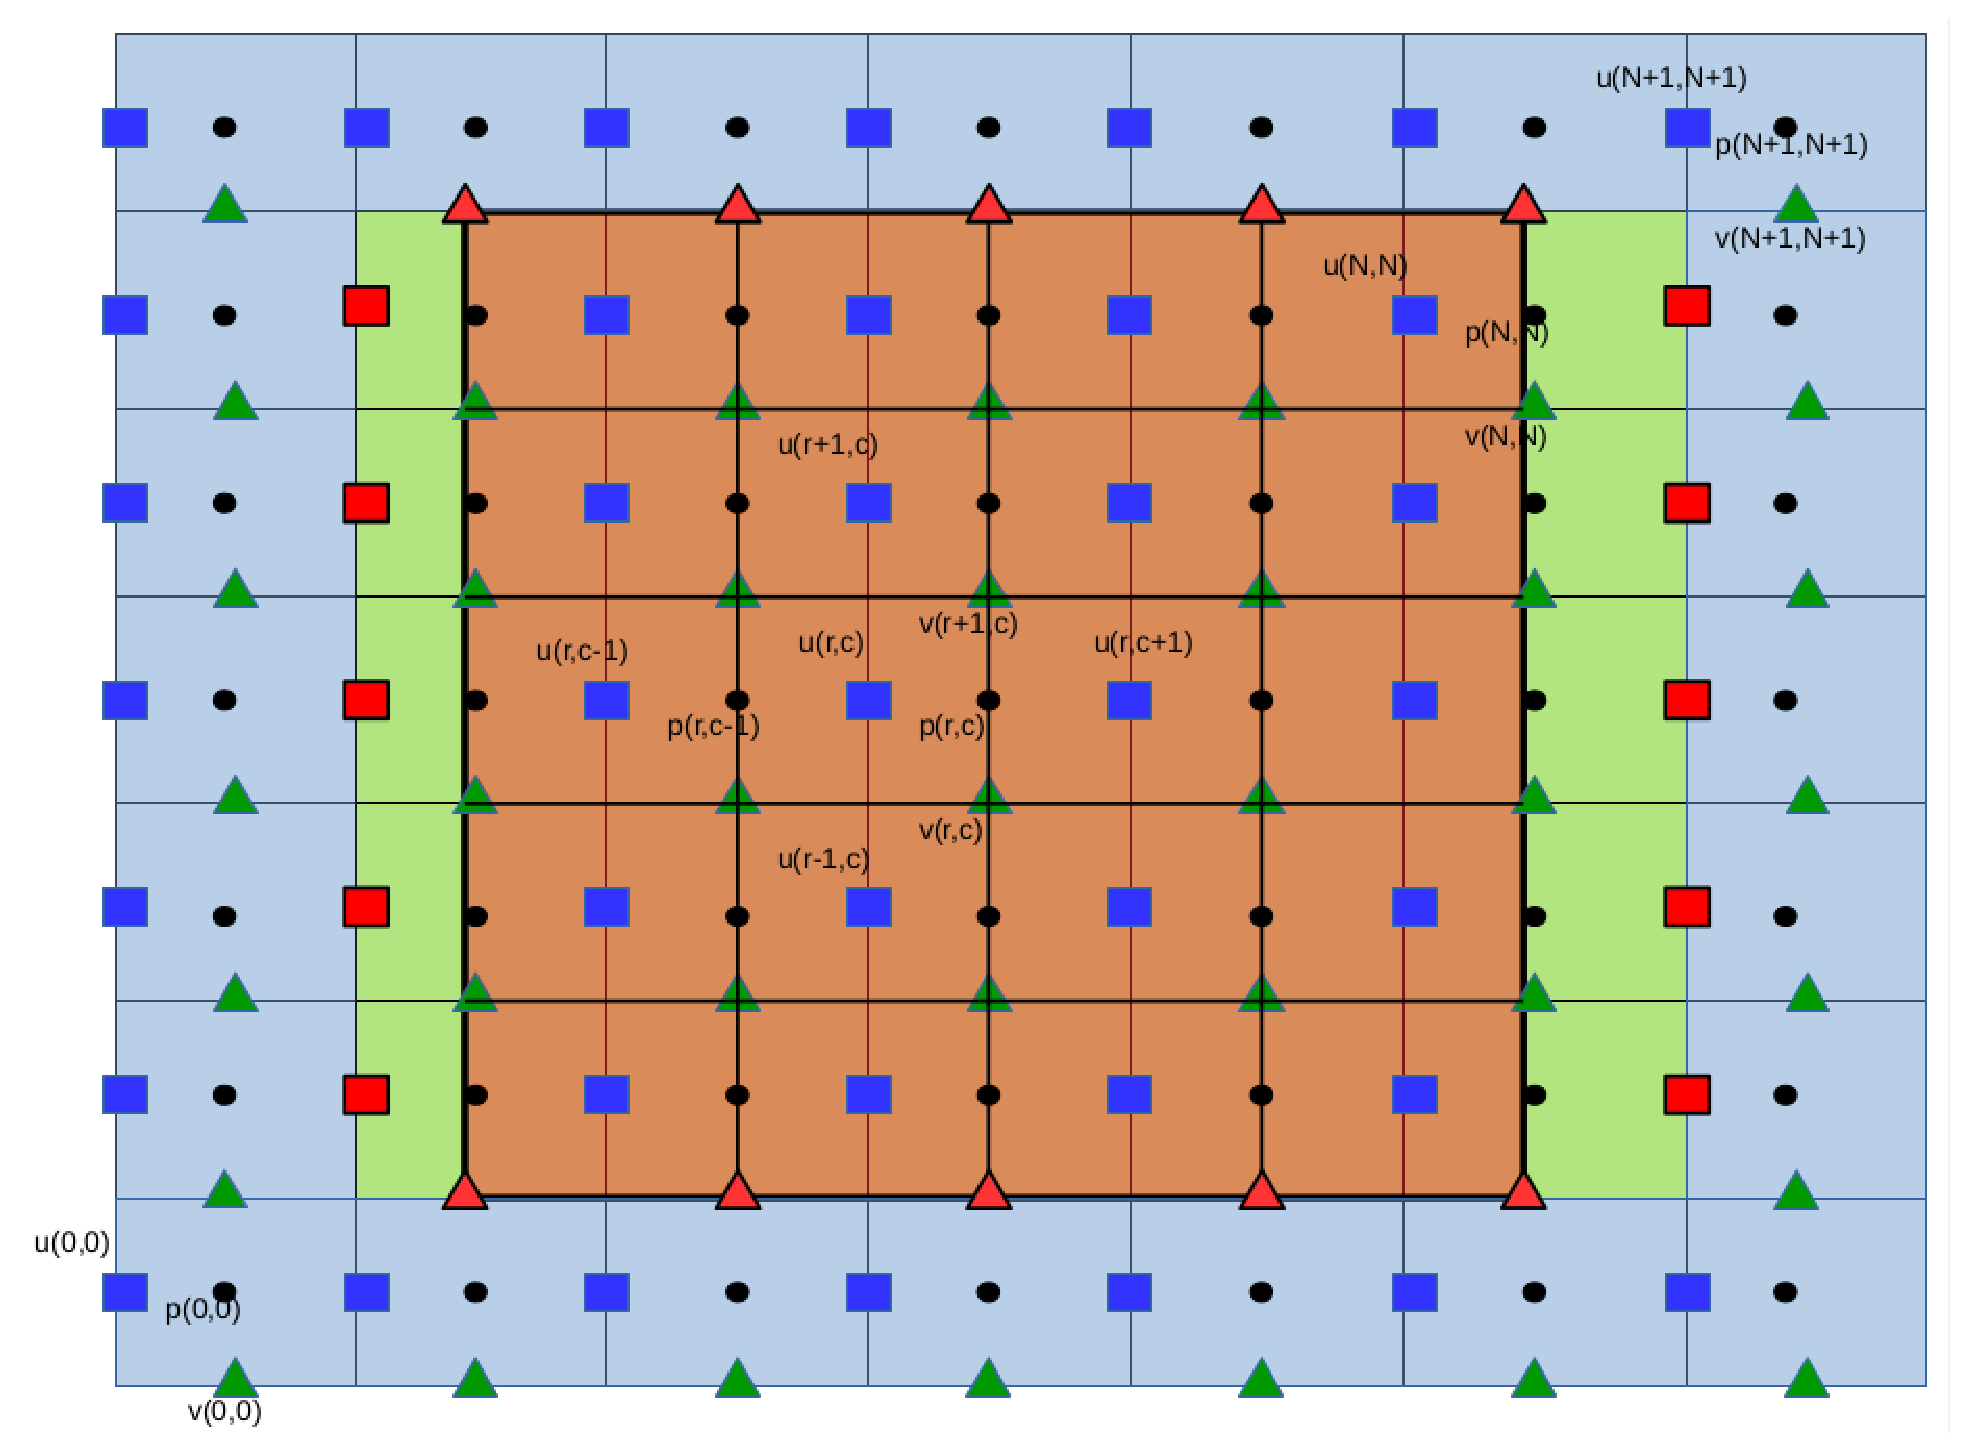
\includegraphics[width=0.8\textwidth]{xvel_calc.eps}
%       }	\\
% \subfloat[Staggered grid for calculation of y-velocity ]{%
%       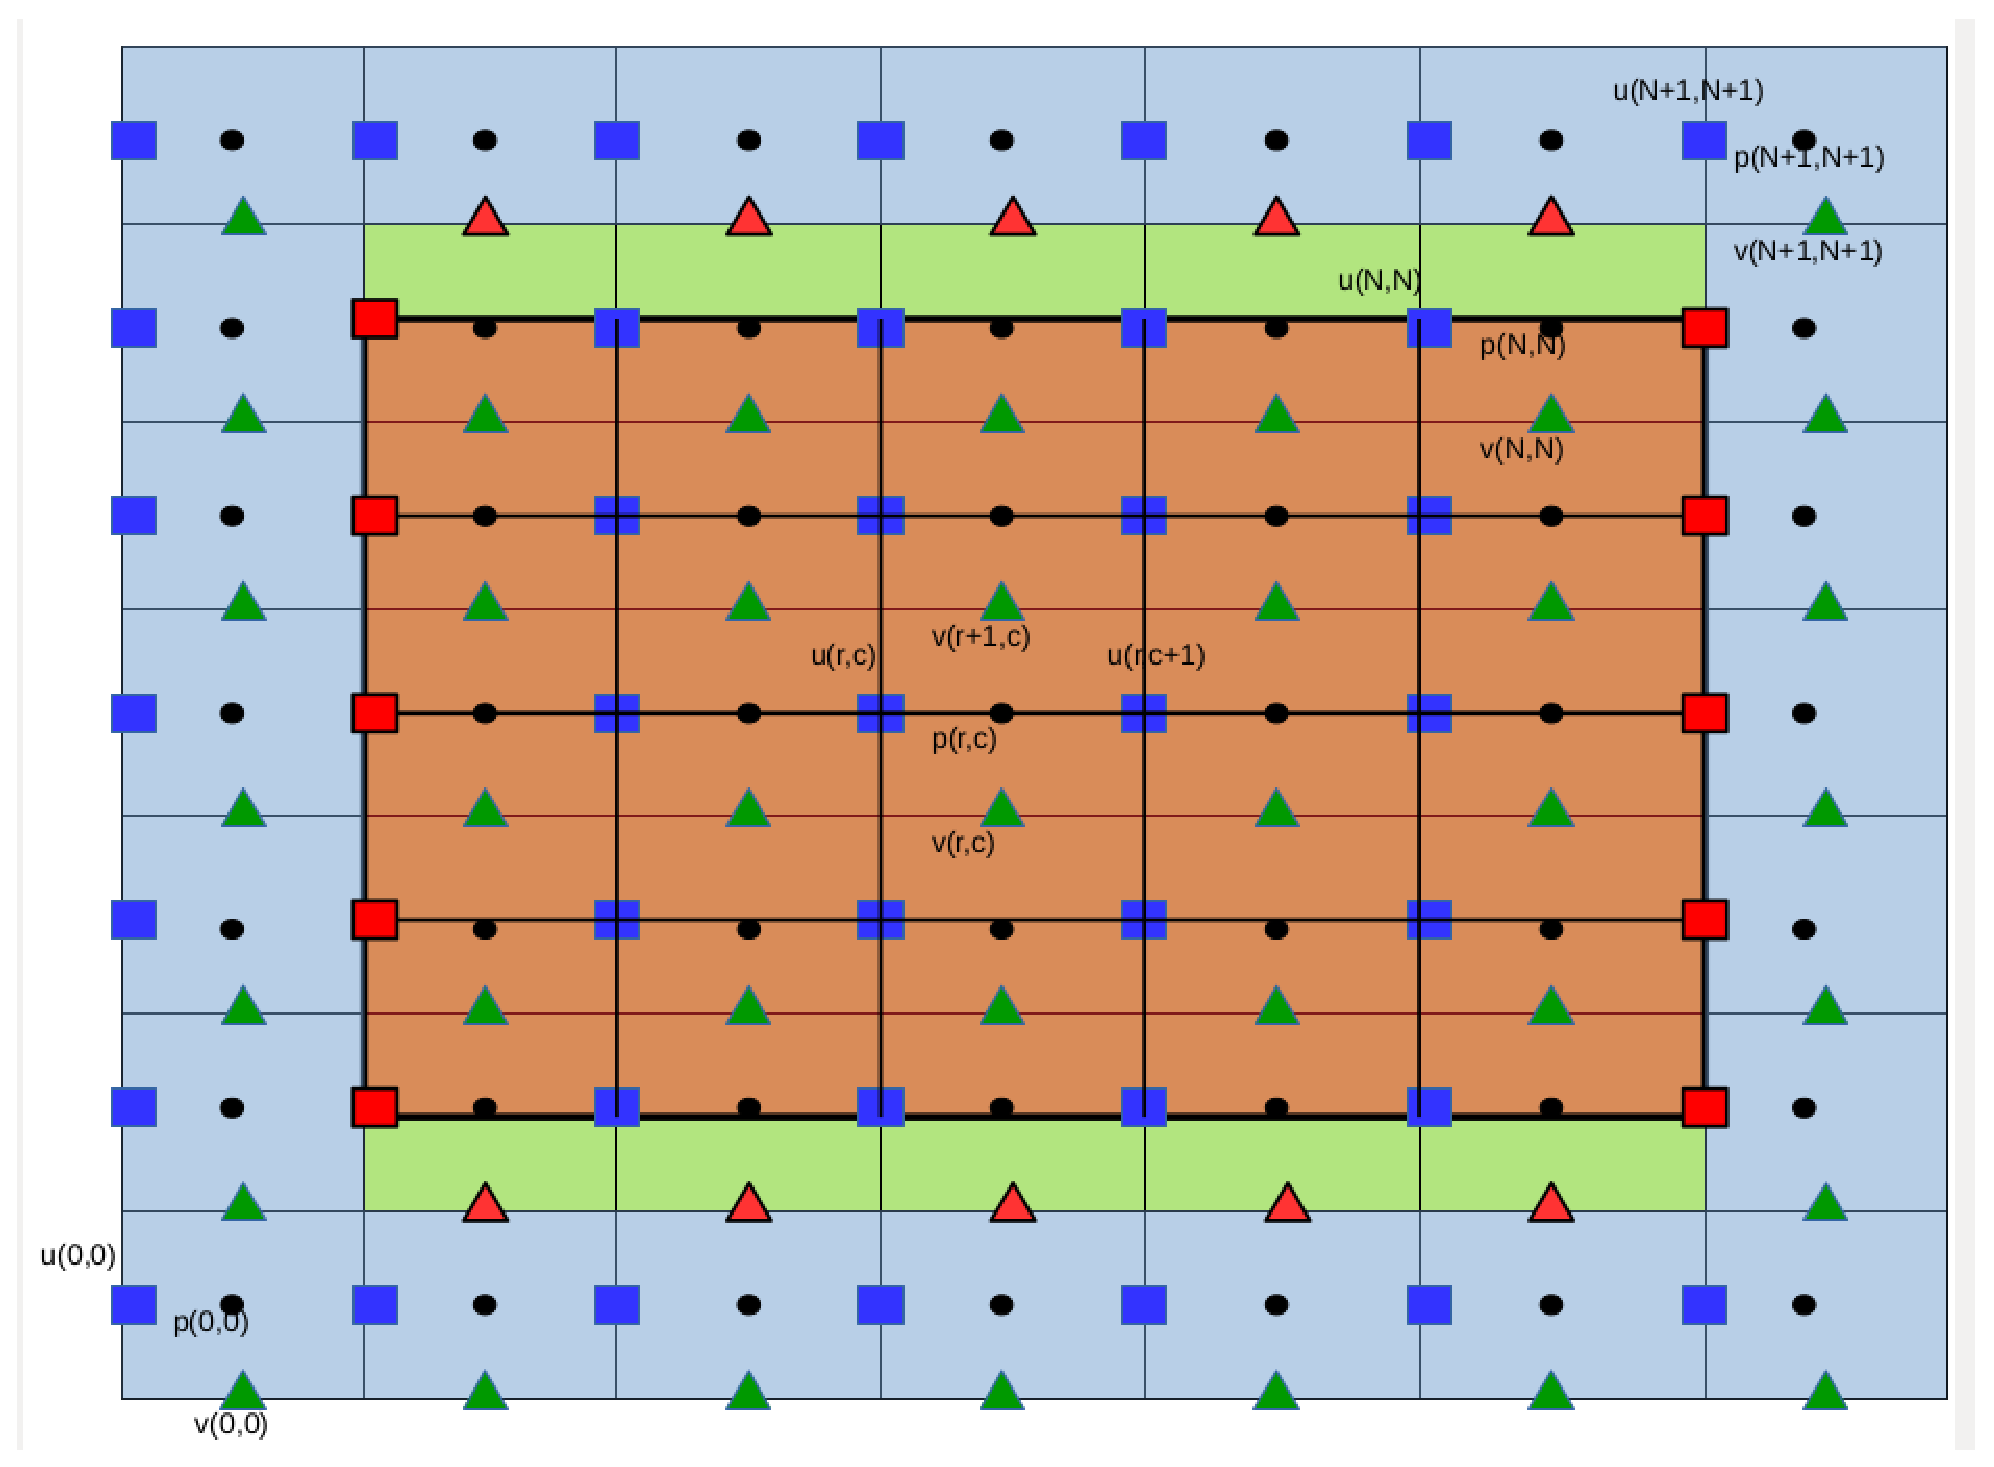
\includegraphics[width=0.8\textwidth]{yvel_calc.eps}
%       }
%       \caption{Different Computational grids for x and y velocity}
% \end{figure}
\subsubsection{Dirichlet Boundary Conditions}
The most commonly used boundary condition is the no-slip on the boundaries, we can set the velocity variables on the boundary to zero or any other value. On the left boundary of the 
domain, the x-velocities are defined so we can set them zero directly, but to set y-velocities we set the ghost control volumes y-velocities to change so that the average of ghost and 
the boundary control volume value becomes zero which is at the wall. This has to implemented inside the time loop, and ghost value has to be updated at every time step 

\begin{equation*}
 \boxed {\begin{align}
  v_{wall} &= \frac{v_{r,0}+v_{r,1}}{2} \\
 v_{r,0}&= 2v_{wall}-v_{r,1}
 \end{align} }
\end{equation*}

The similar operation is used for x-velocities at bottom and top boundaries.

\subsubsection{Neumann Boundary Conditions}
\label{sec:bc}
Conditions are where normal derivative for tangential component of velocity on the wall is zero, and normal component of
velocity on the wall is zero. This is equivalent to free slip, impermeable boundary, also called as symmetry condition. Mathematically, for left wall
\begin{equation*}
 \boxed{ \begin{align}
\frac{\partial v}{\partial x} = 0 \qquad\text{Neumann} \\
 u_{wall} = 0	\qquad\text{Dirichlet}
 \end{align} }
\end{equation*}
To implement the above Neumann condition, on say left wall, we set the following in our code,
\begin{equation*}
 \boxed{ v_{r,0}= v_{r,1} }
\end{equation*}
  
  \section{Pressure Poisson Equation(PPE)}
  For incompressible fluids, it can be followed from \ref{Eq:6} that,
  \begin{equation}
 \nabla .u^{n+1} = 0
 \label{Eq:35}
\end{equation}
\begin{equation*}
\begin{align}
  \nabla \cdot u^{n+1} = \nabla \cdot \left(u^*-\frac{\Delta t}{V}\int_V\frac{1}{\rho}\nabla  p^{n+1} dV\right) = 0 \\
 \nabla \cdot \left(\frac{\Delta t}{V}\int_V\frac{1}{\rho}\nabla  p^{n+1} dV\right) = \nabla \cdot u^*
  \end{align}
\end{equation*}

  \begin{equation}
 \frac{u_{r,c+1}^{n+1}-u_{r,c}^{n+1}}{\Delta x} + \frac{v_{r+1,c}^{n+1}-v_{r,c}^{n+1}}{\Delta y} = 0
\end{equation}
It essentially states that, any solution of velocity field should comply mass conservation, and the velocity field thus obtained must be divergence free. 
substituting (33) in (46), we get

\begin{eqnarray*}
 \frac{1}{\Delta x}\left[u_{r,c+1}^*-\frac{2\Delta t }{(\rho_{r,c}+\rho_{r,c+1})}\left(\frac{p_{r,c+1}-p_{r,c}}{\Delta x}\right) \right.	\\
- \left. u_{r,c}^*+\frac{2\Delta t }{(\rho_{r,c}+\rho_{r,c-1})}\left(\frac{p_{r,c}-p_{r,c-1}}{\Delta x}\right)\right]	\\
+\frac{1}{\Delta y}\left[v_{r+1,c}^*-\frac{2\Delta t }{(\rho_{r+1,c}+\rho_{r,c})}\left(\frac{p_{r+1,c}-p_{r,c}}{\Delta y}\right) \right.	\\
-\left. v_{r,c}^*+\frac{2\Delta t }{(\rho_{r,c}+\rho_{r-1,c})}\left(\frac{p_{r,c}-p_{r-1,c}}{\Delta y}\right)\right]	=0
\end{eqnarray*}
From which we obtain,
 \begin{eqnarray*}
p_{r,c} = \left[\frac{1}{(\Delta x)^2}\left(\frac{1}{\rho_{r,c+1}+\rho_{r,c}}+\frac{1}{\rho_{r,c}+\rho_{r,c-1}}\right)
+\frac{1}{(\Delta y)^2}\left(\frac{1}{\rho_{r+1,c}+\rho_{r,c}}+\frac{1}{\rho_{r,c}+\rho_{r-1,c}}\right)\right]^{-1} \\
\left\{\frac{1}{(\Delta x)^2}\left(\frac{p_{r,c+1}}{\rho_{r,c+1}+\rho_{r,c}}+\frac{p_{r,c-1}}{\rho_{r,c}+\rho_{r,c-1}}\right)\right.
\left.+\frac{1}{(\Delta y)^2}\left(\frac{p_{r+1,c}}{\rho_{r+1,c}+\rho_{r,c}}+\frac{p_{r-1,c}}{\rho_{r,c}+\rho_{r-1,c}}\right)\right. \\
-\frac{1}{2\Delta t}\left. \left(\frac{u_{r,c+1}^*-u_{r,c}^*}{\Delta x} +\frac{v_{r+1,c}^*-v_{r,c}^*}{\Delta y}\right)\right\}
 \end{eqnarray*}

\subsection{Successive Over Relaxation method (SOR)}
Successive over relaxation method is used to solve a linear system of equations derived by extrapolating the Gauss-Sidel method. This extrapolation 
takes the form of a weighted average between the previous iterate and the computed Gauss-Seidel iterate successively for each component.
\begin{eqnarray*}
 y_i^k = \omega \overline{y}_i^k + (1-\omega)y_i^{k-1} 
\end{eqnarray*}
where $\overline{y}_i^k$, denotes the Gauss-Sidel iterate and $\omega$ is the relaxation parameter which is used to accelerate the convergence.
\begin{eqnarray*}
 p_{r,c}^{\alpha+1} = \omega \left[\frac{1}{(\Delta x)^2}\left(\frac{1}{\rho_{r,c+1}+\rho_{r,c}}+\frac{1}{\rho_{r,c}+\rho_{r,c-1}}\right)
+\frac{1}{(\Delta y)^2}\left(\frac{1}{\rho_{r+1,c}+\rho_{r,c}}+\frac{1}{\rho_{r,c}+\rho_{r-1,c}}\right)\right]^{-1} \\
\left\{\frac{1}{(\Delta x)^2}\left(\frac{p_{r,c+1}}{\rho_{r,c+1}+\rho_{r,c}}+\frac{p_{r,c-1}}{\rho_{r,c}+\rho_{r,c-1}}\right)\right.
\left.+\frac{1}{(\Delta y)^2}\left(\frac{p_{r+1,c}}{\rho_{r+1,c}+\rho_{r,c}}+\frac{p_{r-1,c}}{\rho_{r,c}+\rho_{r-1,c}}\right)\right. \\
-\frac{1}{2\Delta t}\left. \left(\frac{u_{r,c+1}^*-u_{r,c}^*}{\Delta x} +\frac{u_{r,c+1}^*-u_{r,c}^*}{\Delta x}\right)\right\}\\
+(1-\omega)p_{r,c}^{\alpha}
\end{eqnarray*}

where $\alpha$ is the previous iteration step and $\omega$ is the relaxation parameter, which can take values from 0-2, for overrelaxation it must be greater than 1.
For stability reasons it must be below 2. A choice of $\omega= 1.2 -1.5$ is usually a good compromise between stability and convergence. The advantage to use SOR is its simplicity 
but it converges very slowly. For faster runs we have to more use advanced methods. (\cite{Tryggvason2011})

\subsection{Boundary Conditions for PPE}
There is no explicit boundary condition for pressure needed, rather we use velocity boundary conditions to get pressure at boundary control volumes. (\cite{Tryggvason2011})
thus \ref{Eq:35} at boundary reduces to 
  \begin{equation}
 \frac{u_{r,c+1}^{n+1}-u_{b,r}}{\Delta x} + \frac{v_{r+1,c}^{n+1}-v_{r,c}^{n+1}}{\Delta y} = 0
 \label{Eq:37}
\end{equation}
where $u_{b,r}$, the boundary value of velocity is known by velocity boundary conditions. From \ref{Eq:37}  the $p_{r,c}$ is computed on the boundary and corner control volumes.
   
\section{Coupling VOF and Navier-Stokes solver}
The volume of fluid interface capturing is coupled with the Navier-stokes solver. Figure \ref{Fig:coupling} shows the schematic to couple the interface capturing and Navier-stokes
solver for a time step. The steps followed are discussed in detail below:-
\begin{figure}
 \centering
 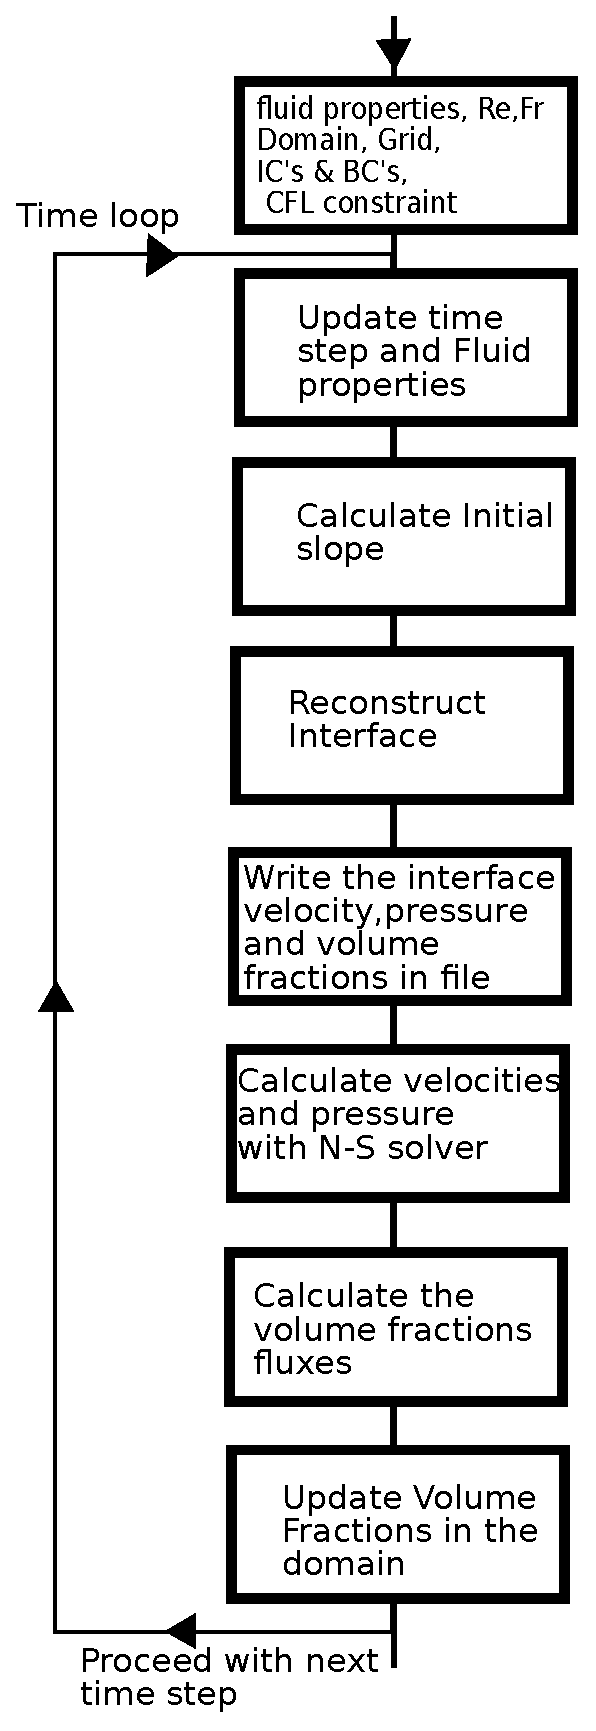
\includegraphics[scale=0.5]{coupling.eps}
 \caption{Sequence to couple VOF and N-S solver}
 \label{Fig:coupling}
\end{figure}

\underline{Input}\\
The solver is fed with following to start the time marching:-
\begin{enumerate}
 \item Initial Volume Fraction field which described the initial condition of the interface
 \item Density ratio of light to the dark fluid, $\tilde\mu = \frac{\rho_G}{\rho_L}$ %($F_{light}=0 \qquad F_{dark}=1$)
 \item Viscosity ratio of light to dark fluid, $\tilde\mu = \frac{\mu_G}{\mu_L}$
 \item Reynolds number defined with dark fluid scales $Re = \frac{Lu\rho_L}{\mu_L}$
 \item CFL number
 \item Domain size
 \item Mesh - No of Cells
\end{enumerate}
\underline{Update time step and fluid properties}\\
The time step is varied to follow the CFL criteria to keep the advection scheme numerically stable. The time step is calculated by
\begin{equation}
 \Delta t = CFL\left(\frac{\Delta}{2u_{max}}\right)
\end{equation}
where $u_{max}$ is the maximum velocity in the actual domain. CFL number should be less than 1.\\
The fluid properties i.e. density $\tilde\rho$, and viscosity $\tilde\mu$ field is updated at every time step using the volume fraction field, which describes the properties
of the fluid in the cells where velocities has to be computed.
\begin{eqnarray}
 \rho_{r,c} = F + (1-F)\tilde\rho  \nonumber \\
 \mu_{r,c} = F + (1-F)\tilde\mu 
\end{eqnarray}
\underline{Calculate Initial slope}\\
Initial guess is calculated using Green-Gauss gradient given by the Equation \ref{Eq:GG}\\
\underline{Reconstruct Interface}\\
Reconstruct the interface using the LVIRA in all the cells in the actual domain.\\
\underline{Write the data}\\
Following data is stored in a file at required intervals. This file can be used to restart the simulation and march further in time.
\begin{enumerate}
 \item x-velocity
 \item y-velocity
 \item Pressure
 \item Volume Fraction
\end{enumerate}
Interface information i.e. the coordinates of the lines in the domain is stored in a different file.\\
\underline{Calculate velocities}\\
The x and y velocities are calculated using the projection method as discussed above in this chapter.\\
\underline{Calculate the volume fraction fluxes}\\
The fluxes are calculated in all the cells actual domain using the velocity field calculated in previous step.\\
\underline{Update the volume fractions}\\
The volume fractions are updated using the fluxes calculated above and the proceed to next time step in the loop by updating the fluid properties with 
updated volume fractions.

\section{Verification}
The test problems were set without any surface tension model and compared with respective available data.
\subsection{Lid Driven Cavity test}
A problem was set test lid driven cavity to get a steady state solution. A square domain of unit length, single fluid and Reynolds number 100, 400, 1000.
The results are validated by \cite{Ghia1982}. Figure \ref{Fig:xyvel1000} shows the x-velocity along vertical center-line and y-velocity along horizontal center-line respectively in the domain. 
Stream function and vorticity contours are shown in Figure \ref{Fig:cont1000}.
\begin{figure}
\centering
  \subfloat[x-velocity along vertical centerline (Re=100) ]{%
      \includegraphics[width=0.5\textwidth]{Re100u.eps}
      }	
 \subfloat[y-velocity along horizontal centerline (Re=100) ]{%
      \includegraphics[width=0.5\textwidth]{Re100v.eps}
      }\\
  \subfloat[x-velocity along vertical centerline (Re=400) ]{%
      \includegraphics[width=0.5\textwidth]{Re400u.eps}
      }	
 \subfloat[y-velocity along horizontal centerline (Re=400) ]{%
      \includegraphics[width=0.5\textwidth]{Re400v.eps}
      }\\
  \subfloat[x-velocity along vertical centerline (Re=1000) ]{%
      \includegraphics[width=0.5\textwidth]{Re1000u.eps}
      }	
 \subfloat[y-velocity along horizontal centerline (Re=1000) ]{%
      \includegraphics[width=0.5\textwidth]{Re1000v.eps}
      }
 \caption{Blue:\cite{Ghia1982}, Red:Present Study(LVIRA)}
 \label{Fig:xyvel1000}
\end{figure}

\begin{figure}
\centering
  \subfloat[Stream function contours at Re=100 ]{%
      \includegraphics[width=0.4\textwidth]{Re100_streamf.eps}
      }	
 \subfloat[Vorticity contours at Re=100 ]{%
      \includegraphics[width=0.4\textwidth]{Re100_vortf.eps}
      }\\
  \subfloat[Stream function contours at Re=400 ]{%
      \includegraphics[width=0.4\textwidth]{Re400_streamf.eps}
      }	
 \subfloat[Vorticity contours at Re=100 ]{%
      \includegraphics[width=0.4\textwidth]{Re400_vortf.eps}
      } \\
  \subfloat[Stream function contours at Re=1000 ]{%
      \includegraphics[width=0.4\textwidth]{Re1000_streamf.eps}
      }	
 \subfloat[Vorticity contours at Re=1000 ]{%
      \includegraphics[width=0.4\textwidth]{Re1000_vortf.eps}
      }
 \caption{Stream function and vorticity contours}
 \label{Fig:cont1000}
\end{figure}

  \subsection{Falling Droplet}
 Falling droplet problem was set up and compared with Gerris simulations with exactly same input conditions (See Figure \ref{fd}).
 \begin{itemize}
 \item Domain: [0,3] x [0,3]
 \item Droplet: Diameter = 0.3, Center (1.5,2.5)
 \item Grid size: 96 x 96
 \item Time Step 0.00125
 \item Density ratio $\frac{\rho_G}{\rho_L}$, $\tilde\rho=0.5$
 \item Viscosity ratio $\frac{\mu_G}{\mu_L}$, $\tilde\mu=1.0$ 
 \item $Re_L=100$
 \item $Fr = 0.1$
  \item Boundary Condition : All walls no slip
 \end{itemize}
 
\begin{figure}
\subfloat[t = 0 ]{%
      \includegraphics[width=0.5\textwidth]{drop_fall_0.eps}
      }
      \subfloat[t = 0.125 ]{%
      \includegraphics[width=0.5\textwidth]{drop_fall_100.eps}
      } \\
      \subfloat[t = 0.25 ]{%
      \includegraphics[width=0.5\textwidth]{drop_fall_200.eps}
      }
      \subfloat[t = 0.375 ]{%
      \includegraphics[width=0.5\textwidth]{drop_fall_300.eps}
      }
 \caption{Falling Droplet test, (Blue-Gerris, Red-Present Study(LVIRA))}
 \label{fd}
 \end{figure}
  
  \subsection{Rayleigh-Taylor Instability}
  Rayleigh-Taylor Instability is one of the most common test problems which are studied for verification, the problem was set up as in \cite{Rudman1997}
   \begin{enumerate}
 \item Domain: [0,1] x [0,3]
 \item Initial Interface: $y=2-0.02cos(\pi x)$
 \item Grid size: 64 x 192
 \item Time Step 0.005
 \item Density ratio $\frac{\rho_G}{\rho_L}$, $\tilde\rho=\frac{5}{6}$
 \item Viscosity ratio $\frac{\mu_G}{\mu_L}$, $\tilde\mu=1.0$ 
 \item $Re_L=500$
 \item $Fr = 0.5$
  \item Boundary Condition : top,bottom and right wall as no slip, left wall free slip
 \end{enumerate}
 Results are shown in Figure \ref{Fig:rudman}
 \begin{figure}
 \centering
 \subfloat[t = 0 ]{%
      \includegraphics[width=0.3\textwidth]{Rudman_t0.eps}
      }
  \subfloat[t = 4 ]{%
      \includegraphics[width=0.3\textwidth]{Rudman_t4.eps}
      } \\
       \subfloat[t = 6 ]{%
      \includegraphics[width=0.3\textwidth]{Rudman_t6.eps}
      }
       \subfloat[t = 8 ]{%
      \includegraphics[width=0.3\textwidth]{Rudman_t8.eps}
      }
 \caption{Comparison of Rayleigh-Taylor Instability test,(Blue-\cite{Rudman1997}, Red-Present Study(LVIRA))}
  \label{Fig:rudman}
 \end{figure}
 
 Similar problem with different initial and boundary conditions was studies and compared with \cite{Anton2001} as shown in Figure \ref{Fig:anton}
    \begin{enumerate}
 \item Domain: [0,1] x [0,4]
 \item Initial Interface: $y=2+0.05cos(2\pi x)$
 \item Grid size: 40 x 160
 \item Time Step 0.001
 \item Density ratio $\frac{\rho_G}{\rho_L}$, $\tilde\rho=\frac{17}{120}$
 \item Viscosity ratio $\frac{\mu_G}{\mu_L}$, $\tilde\mu=1.0$ 
 \item $Re_L=\frac{1000}{3}$
 \item $Fr = 1.0$
 \item Boundary Condition : top and bottom wall as no slip, left and right wall free slip
 \end{enumerate}
 
  \begin{figure}
 \centering
 \subfloat[t = 0 ]{%
      \includegraphics[width=0.3\textwidth]{anton-t0.0.eps}
      }
  \subfloat[t = 1.9 ]{%
      \includegraphics[width=0.3\textwidth]{anton-t1.9.eps}
      } \\
       \subfloat[t = 2.6 ]{%
      \includegraphics[width=0.3\textwidth]{anton-t2.6.eps}
      }
       \subfloat[t = 3.3 ]{%
      \includegraphics[width=0.3\textwidth]{anton-t3.3.eps}
      }
    \subfloat[t = 4.0 ]{%
      \includegraphics[width=0.3\textwidth]{anton-t4.0.eps}
      }
 \caption{Comparison of Rayleigh-Taylor Instability test,(Blue-\cite{Anton2001}, Red-Present Study(LVIRA))}
 \label{Fig:anton}
 \end{figure}
 
\section{Conclusion} 
 The solver however produce satisfactory results while benchmarking but there is a need to improve the accuracy,
 for which we plan to implement advance advection schemes such as Godunov scheme.
 Also, Gauss-Sidel method used to solve pressure poisson equation converges very slowly
 and results in extensive use of computational resources and time. 
 To improve the effciency, we plan to use multigrid methods to solve the pressure poisson equation.
 
 
 
 
 
 
 %
\chapter{Superhydrophobic Droplet Impact - Comparison with Gerris simulations}

\section{Contact angle}
\begin{wrapfigure}{r}{0.5\textwidth}
  \begin{center}
    \includegraphics[width=0.48\textwidth]{Contact_angle.eps}
  \end{center}
  \caption{Contact Angle}
  \label{Fig:Contact_angle}
\end{wrapfigure}
When a gas-liquid interface meets a solid surface, at the point of contact of three phases the liquid makes an angle with the surface. This measures the wettability of 
the solid surface for that liquid. The contact angle is given by Young's equation, ( See Figure \ref{Fig:Contact_angle} ). 
\begin{equation}
 \boxed{ \begin{align}
 &\gamma_{SG} -\gamma_{SL} - \gamma_{LG} \cos \theta =0  \\
 &\cos \theta =\frac{\gamma_{SG} -\gamma_{SL}}{\gamma_{LG}} 
 \end{align}
 }
 \label{Eq:youngs}
\end{equation}
which expresses the balance of forces acting on the contact line in the direction normal to the contact line and tangential
to the solid surface. Experiments show that the contact angle deviates from its static value when
the contact line is in motion. This deviation is an important feature of the problem and needs to be taken into account to obtain realistic answers.\\
\underline{\textbf{Superhydrophobic surfaces}}\par
The effect of the dynamic contact angle and moving contact line however can be made minimal if the spreading of the droplet is very less. Such phenomenon is seen in non-wetting surfaces. 
Surfaces which are extremely difficult to wet are known as superhydrophobic surfaces. \cite{wang2007definition} has attempted to define the superhydrophobic surfaces as the
surfaces that exhibit static contact angle greater than $150^o$. In the next sections we compared some experimental studies on superhydrophobic surfaces with simulations done on Gerris.
% \begin{figure}
% \centering
%     \includegraphics[width=0.48\textwidth]{Contact_angle.eps}
%   \caption{Contact angle}
%   \label{Fig:Contact_angle}
% \end{figure}

\section{Gerris}
Gerris is an open source code created by \cite{Popinet2003} which solves Navier stokes equation using a VOF method for constructing the interface.
\begin{equation}
 \boxed {\begin{align}
 \frac{d \tilde u}{d\tilde t} &= \frac{1}{\rho_k} \left\{ - \tilde \nabla p + \frac{1}{Re_L}  \tilde \nabla \cdot ( \mu_k (\tilde \nabla \tilde u + \nabla \tilde u^T )) 
 + \frac{1}{We_L} \kappa \delta_s \overrightarrow n \right\} + \frac{1}{Fr^2} \\
 \tilde \nabla . \tilde u &= 0 \qquad\text{(Equation of continuity)}\\
 \frac{D\tilde F}{D\tilde t}&=0 \qquad\text{(Volume of Fluid advection equation)}
\end{align} }
\label{Eq:gerris_nd}
\end{equation}
where, 
 \begin{table}[H]
  \begin{center}
   \caption{Variables symbols}
 \label{variables}
    \begin{tabular}{ll}
      \toprule 
	  Variable & Remark   \\ 
	  \midrule
	  $\rho_L$ & Density of liquid  \\ 
	    $\rho_g$ & Density of gas \\
	    $\mu_L$ & Viscosity of liquid  \\
	    $\mu_G$ & Viscosity of gas \\
	     $\frac{\rho_G}{\rho_L}$ & Density ratio gas to liquid \\
	    $\frac{\mu_L}{\mu_L}$ & Viscosity ratio gas to liquid  \\
	    $\sigma_{LG}$ & Surface tension of Liquid-gas   \\
	    $D$ & Diameter of the droplet  \\
	    $g$ & Acceleration due to gravity \\
      \bottomrule \\
    \end{tabular}
  \end{center}
\end{table}
 
\begin{equation*}
\begin{align}
&Re_L = \frac{\rho_L D U}{\mu_L}  &\textbf{(Reynolds Number)}\\
&We_L = \frac{\rho_L D U}{\mu_L}  &\textbf{(Weber Number)}\\ 
&Fr = \frac{U}{\sqrt{gD}}  &\textbf{(Froude Number)}\\
\end{align}
\end{equation*}

The primary current limitation of Gerris flow solver is it does not have \textbf{Dynamic Contact Angle (DCA)} model. In order to find out if lack of dynamic contact angle model affects 
droplet spreading on superhydrophobic surfaces, we compare Gerris simulation with experimental data from \cite{Hung2011}, \cite{Clanet2004} and \cite{Wang2007}
having no-slip conditions and static contact angle at the surface.

\subsection{Simulations}

The problems studied for comparison has the parameters given in Table \ref{parameters} \\

 \begin{table}[H]
  \begin{center}
    \begin{tabular}{ccccccc}
      \toprule 
      Author(s) & $Re_L$ & $We_L$ & $Fr$ & $\rho_k$ & $\mu_k$ & Contact Angle \\ 
      \midrule
      \cite{Hung2011} & 2521 & 29 & 5 & $2 X 10^{-3}$ &  $2 X 10^{-2}$ & $150^{\circ}$ \\
       \cite{Clanet2004} & 2327 & 24 & 5 & $2 X 10^{-3}$ &  $2 X 10^{-2}$ & $170^{\circ}$ \\
        \cite{Wang2007} & 1256 & 9 & 4 & $2 X 10^{-3}$ &  $2 X 10^{-2}$ & $163^{\circ}$\\
      \bottomrule \\
    \end{tabular}
       \caption{Input to solver}
 \label{parameters}
  \end{center}
\end{table}

\underline{Boundary Conditions}: No slip conditions on all walls except axis of symmetry where we use symmetry conditions (described in section \ref{sec:bc}). Impact surface
has a static contact angle.
\subsubsection{\textbf{Gerris simulation vs \cite{Hung2011}}}
\begin{figure}
 \centering
 \subfloat[t = 0.0357 ]{%
      \includegraphics[width=0.3\textwidth]{hung-1.eps}
      }
  \subfloat[t = 0.0361 ]{%
      \includegraphics[width=0.3\textwidth]{hung-2.eps}
      } 
       \subfloat[t = 0.0362 ]{%
      \includegraphics[width=0.3\textwidth]{hung-3.eps}
      }\\
       \subfloat[t = 0.0365 ]{%
      \includegraphics[width=0.3\textwidth]{hung-4.eps}
      }
    \subfloat[t = 0.0368 ]{%
      \includegraphics[width=0.3\textwidth]{hung-5.eps}
      }
       \subfloat[t = 0.0371 ]{%
      \includegraphics[width=0.3\textwidth]{hung-6.eps}
      }\\
       \subfloat[t = 0.0374 ]{%
      \includegraphics[width=0.3\textwidth]{hung-7.eps}
      }
       \subfloat[t = 0.0377 ]{%
      \includegraphics[width=0.3\textwidth]{hung-8.eps}
      }
       \subfloat[t = 0.0379 ]{%
      \includegraphics[width=0.3\textwidth]{hung-9.eps}
      }\\
%        \subfloat[t = 0.0382 ]{%
%       \includegraphics[width=0.3\textwidth]{hung-10.eps}
%       }
 \caption{Interface and center of mass Gerris simulation data(blue) with \cite{Hung2011} experimental data(red), Contact Angle $150^o$}
 \label{Fig:gs5}
 \end{figure}

The interface points and center of mass from the experimental data (\cite{Hung2011}) were extracted and compared with Gerris simulation data. 
The simulation results are seen to be in agreement with experiments before impact. Just after impact (See Figure \ref{Fig:gs5} (a),(b)) the contact line and the contact angle coincides with 
the experimental data but as the contact line starts to move, the simulation interface does not move because of the no slip boundary condition. From (c) to (i) it is seen that
the results are somewhat different from what is observed in the experiment. The vertical position of center of mass is less sensitive to the impact surface.
Figure \ref{Fig:y_com} shows the variation of vertical height of center of mass of droplet with respect to time. It looks like a damped oscillation.

\subsubsection{\textbf{Gerris simulation vs \cite{Clanet2004}}}
\begin{figure}[H]
 \centering
 \subfloat[t = 26.2 ]{%
      \includegraphics[width=0.3\textwidth]{clanet-1.eps}
      }
  \subfloat[t = 27.1 ]{%
      \includegraphics[width=0.3\textwidth]{clanet-2.eps}
      } 
       \subfloat[t = 28.0 ]{%
      \includegraphics[width=0.3\textwidth]{clanet-3.eps}
      }\\
       \subfloat[t = 28.9 ]{%
      \includegraphics[width=0.3\textwidth]{clanet-4.eps}
      }
    \subfloat[t = 29.8 ]{%
      \includegraphics[width=0.3\textwidth]{clanet-5.eps}
      }
       \subfloat[t = 30.7 ]{%
      \includegraphics[width=0.3\textwidth]{clanet-6.eps}
      }\\
       \subfloat[t = 31.6 ]{%
      \includegraphics[width=0.3\textwidth]{clanet-7.eps}
      }
       \subfloat[t = 32.5 ]{%
      \includegraphics[width=0.3\textwidth]{clanet-8.eps}
      }
       \subfloat[t = 33.4 ]{%
      \includegraphics[width=0.3\textwidth]{clanet-9.eps}
      }
 \caption{Interface Gerris simulation data(blue) with \cite{Clanet2004} experimental data(red) Contact Angle $170^o$}
 \label{Fig:gs6}
 \end{figure}
  \cite{Clanet2004} showed that droplet impacting on superhydrophobic surfaces behaves like a balloon filled with fluid in some regime of parameters,
 where the movement of contact line is restricted and the boundary condition for velocity can be taken as no-slip. 
 This study involved superhydrophobic surfaces with contact angle of  $170^o$. We made a comparison with Gerris simulation with static contact angle
 boundary condition and no slip  at surface (See Figure \ref{Fig:gs6} and \ref{Fig:y_com_clanet}). It can be seen that superhydrophobic surfaces has very little
 spreading and has minimal effect on 
 the dynamics of droplet impact.
  \begin{figure}[H]
  \centering
 \includegraphics[scale=0.2]{y_com_clanet.eps}
 \caption{y coordinate of center of mass of droplet to time. blue-Gerris, red-\cite{Clanet2004}}
 \label{Fig:y_com_clanet}
\end{figure}

 \subsubsection{\textbf{Gerris simulation vs \cite{Wang2007}}}
 A comparison with \cite{Wang2007} (See Figure \ref{Fig:gs7}), the surface has a contact angle of $163^o$, also corroborate the fact that the static contact angle conditions
are a good approximation for the solution of droplet impact on superhydrophobic surfaces.\\

 \begin{figure}[H]
 \centering
 \subfloat[t = 15.6 ]{%
      \includegraphics[width=0.3\textwidth]{wang-1.eps}
      }
  \subfloat[t = 16.0 ]{%
      \includegraphics[width=0.3\textwidth]{wang-2.eps}
      } 
       \subfloat[t = 17.0 ]{%
      \includegraphics[width=0.3\textwidth]{wang-3.eps}
      }\\
       \subfloat[t = 18.1 ]{%
      \includegraphics[width=0.3\textwidth]{wang-4.eps}
      }
    \subfloat[t = 19.0 ]{%
      \includegraphics[width=0.3\textwidth]{wang-5.eps}
      }
       \subfloat[t = 19.5 ]{%
      \includegraphics[width=0.3\textwidth]{wang-6.eps}
      }
    \caption{Interface Gerris simulation data(blue) with \cite{Wang2007} experimental data(red) Contact Angle $163^o$ }
 \label{Fig:gs7}
 \end{figure}   
%   \begin{figure}[H]
%  \centering
%  \subfloat[t = 15.6 ]{%
%       \includegraphics[width=0.3\textwidth]{wang-140-1.eps}
%       }
%   \subfloat[t = 16.6 ]{%
%       \includegraphics[width=0.3\textwidth]{wang-140-2.eps}
%       } 
%        \subfloat[t = 17.5 ]{%
%       \includegraphics[width=0.3\textwidth]{wang-140-3.eps}
%       }\\
%        \subfloat[t = 20.4 ]{%
%       \includegraphics[width=0.3\textwidth]{wang-140-4.eps}
%       }
%     \subfloat[t = 21.9 ]{%
%       \includegraphics[width=0.3\textwidth]{wang-140-5.eps}
%       }
%        \subfloat[t = 24.6 ]{%
%       \includegraphics[width=0.3\textwidth]{wang-140-6.eps}
%       }
%     \caption{Interface Gerris simulation data(blue) with \cite{Wang2007} experimental data(red) Contact Angle $140^o$}
%  \label{Fig:gs8}
%  \end{figure}
\begin{figure}
 \centering
 \includegraphics{y_com_hung.eps}
 \caption{y coordinate of center of mass of droplet to time}
 \label{Fig:y_com}
\end{figure}

\section{Conclusion}
Preliminary data seems to suggest that the droplet dynamics and impact on superhydrophobic surfaces is not very sensitive to the precise nature of boundary conditions at the contact line.
Further studies are underway to validate this. Some directions of future research are indicated below:
\begin{enumerate}
\item Motion of center of mass of droplet. 
 \item Droplet impact on inclined plane.
 \item Droplet impact inclined to the plane.
 \item Oscillations of droplet after impact.
 \item Droplet breakup after impact.
\end{enumerate}
As Gerris does not have a dynamic contact angle model, we are in process of developing a multiphase Navier-Stokes solver and to implement 
the dynamic contact line model in it. Our code is expected to mimic droplet impact after implementation of contact model. We plan to explain
some aspects of this phenomena through simple mathematical models.


% \begin{figure}
%  \centering
%  \subfloat[ ]{%
%       \includegraphics[width=0.3\textwidth]{droplet_c1.eps}
%       }
%   \subfloat[t = 27.1 ]{%
%       \includegraphics[width=0.3\textwidth]{droplet_c2.eps}
%       } 
%        \subfloat[t = 28.0 ]{%
%       \includegraphics[width=0.3\textwidth]{droplet_c3.eps}
%       }
%   \caption{Moving contact line during impact}
%   \label{Fig:contact_line}
%   \end{figure}

  \chapter{Multigrid Methods}

\section{Introduction}
In the previous chapter, we encountered Pressure Poisson's Equation (PPE) and used Successive Over Relaxation (SOR) method to reach the solution for pressure.
However, we concluded that SOR has very slow convergence and faster methods should be used to solve the PPE.  Fast Poisson solvers use advanced techniques, 
such as discrete Fast Fourier transform or cyclic reduction, multigrid methods and iterative Krylov-subspace methods. \par
Developed in late eighties (\cite{wesseling1995introduction},\cite{briggs2000multigrid}), Multigrid methods has been used by many authors to solve PPE. We first discuss the characteristics of 
classic iterative methods and then show how the concepts from the analysis can be used to accelerate the convergence, and subsequently state the algorithm which we will 
implement in the solver to solve the PPE. The PPE has to be solved while solving the Navier-Stokes equation which is the most expensive 
part of the solution as it takes most of the time. Hence there is a need to solve this equation efficiently.Multigrid method has been developed for serial processor.

\section{General Iterative Methods}

As the discretised form of Poisson's equation has a system of linear algebric equations. We consider a one dimensional Laplace equation as it is easier to study
analytically. 
\begin{equation}
\frac{d^2u}{dx^2} = 0
\end{equation}
having boundary conditions,
$u(0)=0$ and $u(L) = 0$, which has the exact solution simply $u(x) = 0$. We now look into a numerical method to get the solution of this equation. First we
discretise the differential equation and get algebric equations.
\begin{equation}
\begin{align}
 \frac{u_{i+1}-2u_{i}+u_{i-1}}{h^2} &=& 0 \\
 \text{or,}\quad u_{i+1}-2u_{i}+u_{i-1} &=& 0 \\
 \text{of form,}\quad Ax&=&b
 \end{align}
 \label{E1}
\end{equation}

But the iterative methods don't solve $x = A^{-1} b$, rather the problem is formulated as $x = Px + Q$. These generally differ in the forms of $P$ and $Q$. 
For Gauss-Seidel method, we can split the operator A, as shown in Fig.\ref{Fig:matrix} in strictly lower, diagonal and strictly upper parts i.e. $A = L + D +U$. 
\begin{figure}
 \centering
 \includegraphics[scale=0.2]{mat-A.eps}
 \caption{The matrix A}
 \label{Fig:matrix}
\end{figure}

\begin{equation}
 \begin{align}
  (D +  L + U)x &= b \\
  (D+L)x &= -Ux + b \\
  x^{j+1} &= (D+L)^{-1}(-U) x^j + (D+L)^{-1}b
 \end{align}
\label{E2}
\end{equation}
\vspace{1cm}
From \ref{E2} we can see that $P = (D+L)^{-1}(-U) $ and $ Q = (D+L)^{-1} $. \par

For problem \ref{E1}, the error is defined as $e^j = u^e - u^j$, where $e^j$ is
the the error and $u^j$ is the value of $u$ at j\textsuperscript{th} iteration. The exact answer to the problem is known $u^e = 0$ at all x,
hence the error, is simply  $e^j =  - u^j$. \par
We can now discuss the behavior of Gauss-Seidel method by starting with arbitrary initial guesses. To find the characteristics for different error profiles, we solve the 
problem with initial guesses given by, 
\begin{equation}
 u_i = sin\left(\frac{k\pi x_i}{L}\right)
 \label{E3}
\end{equation}

\begin{figure}
 \centering
 \includegraphics[scale=0.2]{Fourier_modes.eps}
 \caption{Fourier modes}
 \label{Fig:modes}
\end{figure}

In Eq. \ref{E3}, Fourier modes and k is the wavenumber. Fig. \ref{Fig:modes} shows the modes over the domain for k=1, 2 and 8. We can see for low values of k the error is 
smooth and for higher wavenumbers the profiles are oscillatory.

\begin{figure}
\centering
  \subfloat[k=1 ]{%
      \includegraphics[width=0.5\textwidth]{k1.eps}
      }	
 \subfloat[k=2 ]{%
      \includegraphics[width=0.5\textwidth]{k2.eps}
      }\\
  \subfloat[k=3 ]{%
      \includegraphics[width=0.5\textwidth]{k8.eps}
      }	

 \caption{Profile after 10 Gauss-Siedel iterations, Blue - Inital guess, Orange - After 10 iterations}
 \label{Fig:modes_iter}
\end{figure}

In Fig. \ref{Fig:modes_iter}, we can see for a given number of iterations the method converges faster for higher values of wavenumber in the error. 
To know the dependence of wavenumber on the convergence we have to analyse the characteristics of Gauss-Sidel method.

\subsection{Convergence analysis of Gauss-Siedel method}

We know that while approaching to the solution the error approaches to zero. We might want to look how the error decimates with respect to iterations. 
\begin{equation}
 \begin{align}
 e^n = P^n e^0
 \end{align}
 \label{E4}
\end{equation}

Now, if we expand $e^0$ in eigen basis of $P$, we get,
\begin{equation}
 e^0 = \Sigma C_k v_k
\end{equation}
where $C_k$ are the components of $e^0$ in eigen basis of and $v_k$ are eigenvectors of iteration operator $P$. We know that $P$ in its eigenbasis 
will only strech or contract the components when operated on a vector (here $e^0$) by corresponding eigenvalues $\lambda$. Hence, \ref{E4} can be expressed as,

\begin{equation}
 e^n = \Sigma \lambda^n_k C_k v_k
 \label{E5}
\end{equation}

From \ref{E5}, it can be seen that largest value of $|\lambda_k|$ should be less than 1, for the error to approach zero in successive iterations i.e. for convergence. This value is 
known as the spectral radius of the iteration matrix $P$. It can also be concluded from here that the smaller the spectral radius faster the convergence. We have observed in the
previous section that there is faster convergence for high wavenumber errors and we know that convergence is directly affected by the eigenvalues of the $P$ operator. We now look
what is the relation between the wavenumber and the eigenvalues of $P$. \par

The eigenvalues of Jacobi iteration operator is given by,
\begin{equation}
 \lambda_k = 1- sin^2\left(\frac{k\pi}{2N}\right) \hspace{1cm}\text{k = 1,2,...N}
 \label{E6}
\end{equation}

\begin{figure}
 \centering
 \includegraphics[scale=0.2]{eigen_vs_k.eps}
\caption{Eigenvalues$\lambda$ with respect to k}
 \label{Fig:eig_vs_k}
\end{figure}

where N is the number of nodes in the grid. From \ref{E6} we plot $\lambda$ vs k in \ref{Fig:eig_vs_k}, and we can now understand reasons for the results in previous section i.e.
the eigenvalue is low for high wavenumber modes and hence we found faster convergence for high wavenumbers.  In practical problems we don't have the solution, we need to find it and most of the times it is not even possible to give a good guess. Most
of the times we start with zero values of the variable to be calculated. Hence when we start with an arbitrary guess and it can
have errors of many wavenumbers. With this argument we cannot do much about increasing the wavenumber or the oscillatory behavior of the error.
But we can again look at \ref{E6}, the convergence depends on low values of $\lambda$, but it is not entirely dependent on wavenumber k but the ratio $\frac{k}{N}$ 
( See Fig. \ref{Fig:eig_vs_k-N} ).
For a given wavenumber $k =1$, for which convergence is low, See Fig. \ref{Fig:eig_vs_N} it can be said that low wavenumber component will converge faster on coarser grids.
This result lays down the foundation for multigrid methods. In literature we can find many variants of multigrid methods but the prime reason is buried in the dependence of eigenvalues
of the iteration operator on grid size. 


\begin{figure}
 \centering
 \includegraphics[scale=0.2]{eigen_vs_k-N.eps}
 \caption{Eigenvalues$\lambda$ with respect to $\frac{k}{N}$}
 \label{Fig:eig_vs_k-N}
\end{figure}

\begin{figure}
 \centering
 \includegraphics[scale=0.2]{eigen_vs_N.eps}
 \caption{Eigenvalues$\lambda$ with respect to N}
 \label{Fig:eig_vs_N}
\end{figure}


\section{Algorithm of Multigrid method}

In the light of above results, we can think of an strategy to exploit the faster convergence characteristics of the method. It could be to solve the problem on 
coarser grids and interpolate the result on finer grid. This would be a better guess for finer grid and we can repeat the process till the finest grid when we 
want the solution. 
The disadvantages of this strategy are:
\begin{enumerate}
 \item The problem is solved fully on coarser grids even we are only interested in the solution on finest grid.
 \item It does not make use of any guess which we can have from finer grids.
 \item Sometimes the problem is not well resolved on coarser grids and hence the guess provided by the coarser grid solution might not be a good guess.
\end{enumerate}

A better strategy is to coarse grid correction, which calculates the error on coarser grids and provide a correction on the finest grid. We have defined the 
error as:
\begin{equation}
 \begin{align}
  \text{exact solution} \quad Ax^e &= b \\
  \text{solution at k\textsuperscript{th} iteration} \quad Ax^k &= b -r \\
  \text{error at k\textsuperscript{th} iteration} \quad e^k &= x^e - x^k \\
  \text{from above, we get,}\quad A(x^e-x^k) &= r \\
  \text{or,} \quad  Ae^k &= r
 \end{align}
 \label{E7}
\end{equation}

We solve the given problem $Ax = b$ on the finest grid, and $A^e = r$ on the coarser grids. The basic steps in the algorithm are:
\begin{enumerate}
 \item Iterate for few steps the given problem on the finest grid. This step is \textbf{relaxation}. 
 \item Transfer the residue from finest grid to coarser grid. This step is called as \textbf{restriction}.
  \item Interpolate the values of error and add it previous values to make a correction. This step is
    \textbf{prolongation}.
\end{enumerate}

The algorithm for multigrid is followed as in Fig. \ref{Fig:fd_mg}. This is V cycle algorithm, where the restriction is done till the coarsest grid and then prolongation till 
the finest grid.% (See Fig \ref{Fig:Vcycle}). put a V figure for vcycle later.
\begin{figure}
 \centering
 \includegraphics[scale=0.5]{fd_mg.eps}
 \caption{Multigrid Algorithm}
 \label{Fig:fd_mg}
\end{figure}

\section{Sample Problem}

We try to solve to some problems to understand the implementation details of the algorithm. Consider a one dimensional Poisson's equation \ref{E8},
\subsection{One dimensional Poisson's equation}
\begin{equation}
 \frac{d^2 u}{dx^2} = \frac{1}{2}[sin \pi x + sin 16 \pi x]
 \label{E8}
\end{equation}

having boundary conditions $u(0) = u(1) = 0$. We can discretise Eq. \ref{E7} as,

\begin{equation}
 \frac{u_{i+1}-2u_{i}+u_{i-1}}{h^2} = \frac{1}{2}[sin \pi x_i + sin 16 \pi x_i]  
 \label{E9}
\end{equation}

Let the RHS be $q_i$ at i\textsuperscript{th} node. Then we can write for $u_i$ from \ref{E9} as,

\begin{equation}
 u_i^{n+1} = \frac{1}{2}(u_{i+1}^n+u_{i-1}^{n+1}-h^2 q_i)
 \label{E10}
\end{equation}

%Eq. \ref{E10} can be solved using Gauss-Sidel method where we can see the residue at n\textsuperscript{th} iteration in Fig. \ref{Fig:GS}. 

Eq. \ref{E10} is iteration equation for Gauss-Sidel method but for multigrid we iterate only few times. Here we will iterate only once in 
each step in a V-cycle. We have the finest grid having N = 64 with total nodes N + 1 i.e. 65. We now restrict the residue to the coarser
grid which has N/2+1 nodes. We can use average restriction as, 

\begin{equation}
 r^{2h}_i = \frac{1}{4} (r^h_{2i-1} + 2r^h_{2i} + r^h_{2i+1})
 \label{E11}
\end{equation}

Then iterate for error on the coarser grid as,

\begin{equation}
 e_i^{n+1} = \frac{1}{2}(e_{i+1}^n+e_{i-1}^{n+1}-h^2 r_i)
 \label{E12}
\end{equation}

restriction and iteration continues till the coarsest grid. At coarsest grid the iteration the error equation is solved exactly. Then the 
error is interpolated backwards for prolongation step as,

\begin{equation}
\begin{align}
 e^{h}_i &=& e^{2h}_i \quad \text{i = 0,...,N}\\
  e^{h}_{2i+1} &=& \frac{e^{2h}_i +  e^{2h}_{i+1}}{2} \quad \text{i=0,...,N}
 \end{align}
 \label{E11}
\end{equation}

While prolongation iteration step is taken at every grid level and at finest grid, we add the interpolated error to the $u$, again start with 
the V-cycle with the new $u$ as a guess. The results for this problem are compared with \cite{moin2010fundamentals} (See Fig. \ref{Fig:moin1D}).

\begin{figure}
 \centering
 \includegraphics[scale=0.4]{moin_1D.eps}
 \caption{Comparison with Moin(2010)}
 \label{Fig:moin1D}
\end{figure}

\subsection{Two dimensional Poisson's equation}

We are interested in solving the Poisson equation, Equation \ref{eq:Poisson}, in a square domain of size unity centered on
unity with Neumann boundary conditions on all sides (\cite{Popinet2003}).

\begin{equation}
{\nabla}^2 \phi = f(x,y)
\label{eq:Poisson}
\end{equation}

\noindent Source term $f(x,y)$ is given by

\begin{equation}
f(x,y) = -{\pi}^2(k^2+l^2)\sin(\pi k x)\sin(\pi l y)
\label{eq:Source}
\end{equation}

\noindent with $k=l=3$. Exact solution of the Poisson equation with this source term is

\begin{equation}
\phi(x,y) = \sin(\pi k x)\sin(\pi l y) + \kappa
\label{eq:Solution}
\end{equation}

\noindent where $\kappa$ is an arbitary constant.

\section{Discretization}

Problem domain, shown in Figure \ref{fig:discretization}, is discretized using a 2nd-order
finite difference approximation on a cartesian grid having N nodes in both x- and y-directions which correspondes
to a uniform grid spacing h. The value of $\phi$ on the 2D cartesian mesh can then be approximated
for each node {i,j} in the interior of the computational domain as

\begin{equation}
\frac{1}{h^2} \left({{\phi}^n_{i-1,j}} + {{\phi}^n_{i,j-1}} -4 {{\phi}^{n+1}_{i,j}} + {{\phi}^n_{i+1,j}} + {{\phi}^n_{i,j+1}} \right) = f_{i,j}, \hspace{1 cm} i, j = 2,..., N-1
\label{eq:discretization}
\end{equation}

\noindent where the subscripts $i$ and $j$ represent the indices of the current node in the computational domain for the
$x$ and $y$ directions, respectively.

\begin{figure}
\begin{center}
\includegraphics[width=3.0 in]{pressure.eps}
\end{center}
\caption{2D uniform mesh featuring a discretization with a 5-point stencil.}
\label{fig:discretization} 
\end{figure}

\section{Validation}

\begin{figure}
\begin{center}
{\tiny
\begin{tabular}{cc}
\includegraphics[width=4.0in]{sol_N500_np1.eps} \\
(a) \\
\includegraphics[width=4.0in]{err_N500_np1.eps} \\
(b)
\end{tabular}}
\end{center}

\caption{Solver results of for $N=500$ and $np=4$; (a) Poisson solution and (b) solution error.}
\label{fig:dsmc_cfd1}
\end{figure}
\newpage
\section{Comparison with SOR Parallel}
The same problem is solved using SOR (MPI) and the results are compared.

The following tests performed on the a machine having the following specifications:

\begin{enumerate}
 \item Processor:  Intel(R) Xeon(R) CPU E5-1650 v3 @ 3.50GHz
 \item CPU Cores: 6 (6 more with hyperthread-Virtual cores)
 \item RAM:	 64 GB
 \item Cache:    15360 KB
\end{enumerate}

\begin{figure}
\begin{center}
\includegraphics[width=5.0 in]{speedup.eps}
\end{center}
\caption{Speedup values for MPI parallel (SOR) Poisson equation solver.}
\label{speedup} 
\end{figure}

\begin{figure}
\centering
 \includegraphics[scale=0.25]{comparison.eps} 
 \caption{Comparison of SOR and Multigrid Time of execution}
 \label{comparison_mg}
\end{figure}

From Fig.\ref{speedup} it can be observed that time of execution has decreased with increase in number of processors and speed up is more 
for larger size problem. A decrease in speed up is seen when the number of processors were more than the physcial cores and the threads took
more time to process. Fig. \ref{comparison_mg} has emphasizes the fact that multigrid on a single processor is far more efficient on a multicore
SOR algorithm. Hence this work can be further extended for parallelizing the multigrid algorithm.
















 
\chapter{Surface Tension}

\subsection{Height Function}

The height function is calculated as shown in Fig. \ref{height_function} (when absoulute value of y-normal of interface is greater
than x-normal), as
\begin{enumerate}
 \item Start the summation from the middle row
 \item Sum upwards as long as the cells contain dark fluid
 \item Sum downwards as long as the cells contain light fluid,
but subtract one for each cell added
\item The sums result in a histogram which approximates the
interface
\end{enumerate}



The radius of curvature is given by,
\begin{equation}
 \kappa = -\frac{h^{''}(x)}{[1+(h^{'}(x))^2]^{3/_2}}	%{h^{''}(x)} {[1+(h^'(x))^2]^{3/_2}}
\end{equation}


\begin{figure}
 \centering
 \includegraphics[scale=0.6]{height_function.eps}
 \caption{Variable Stencil for calculation of height functions}
 \label{height_function}
\end{figure}

\begin{algorithm}
  \caption{Height Function algorithm}\label{euclid}
  \begin{algorithmic}[1]
    \Procedure{Height}{$F$}\Comment{Volume Fractions as argument}
%       \State $r\gets a\bmod b$
%       \While{$r\not=0$}\Comment{We have the answer if r is 0}
%         \State $a\gets b$
%         \State $b\gets r$
%         \State $r\gets a\bmod b$
%       \EndWhile\label{euclidendwhile}
      \For{\texttt{Traverse through all cells}}
        \State \If{$0<F<1$} \Comment{if cell contains the interface}
        \State $d = max(|nx|,|ny|)$ \Comment {find the direction of maximum normal}
        \State \While {$F>0$} %\Comment{Sum in d direction as long as the cells contain dark fluid}
        \State \texttt{$H = \sum_d F_d$}
        \State $d=d+1$
        \EndWhile
         \State \While {$F>0$} %\Comment{Sum in negative-d direction as long as the cells contain light fluid}
        \State \texttt{$H = \sum_d (F-1)$}
         \State $d=d-1$
        \EndWhile
	 \State \EndIf 
      \EndFor
      \State \textbf{return} $H$\Comment{The Height Function is $H$}
    \EndProcedure
  \end{algorithmic}
\end{algorithm}


\setlength\tabcolsep{1mm}

\begin{table}[t]
  \begin{center}
    \caption{Comparison of spurious currents, The capillary number is computed by different surface tension methods}
    \label{table:bp}
      \begin{tabular}{c c c c c c c c c c}
	\toprule
	Case & $La$ & $\frac{\rho_{liq}}{\rho_{gas}}$ & $\frac{\mu_{liq}}{\mu_{gas}}$ & $\frac{D}{h}$ & CSS & CSF & FT & CSF\footnote{*Present Study} & HF\footnote{ Present Study} \\
	\midrule
	A & 0.357 & 1 & 1 & 32 	& $3x10^{-3}$ & $1.2x10^{-2}$ & $3.0x10^{-4}$ & $1.22x10^{-2}$ & NA \\
	B & $2x10^{6}$ & 1 & 1 & 32 & $3x10^{-4}$ & $5.0x10^{-4}$ & $1.5x10^{-4}$ & disintegrates & NA \\
	C & $2x10^{6}$ & $10^3$ & 1 & 32 & disintegrates & $3.5x10^{-3}$ & $1.1x10^{-3}$ & $1.5x10^{-3}$ & NA \\
	D & $2x10^{6}$ & $10^3$ & 50 & 32 & disintegrates & $4.5x10^{-3}$ & blows up & $1.6x10^{-3}$ & NA \\ 
	\bottomrule
      \end{tabular}
    \end{center}
 \end{table}
 
  \begin{figure}
 \centering
 \includegraphics[scale=0.4]{interfaces_diff_phi.eps}
 \caption{Interface shapes for different values of $\Phi$ using Height Function at $\tau = 6$}
\end{figure}
 
\begin{table}[t]
  \begin{center}
    \caption{Comparison of growth rate n among the various numerical methods(PROST, CLSVOF, $K_8$ and HF) and analytical results with
    respect to relative importance of surface tension $\Phi$}
    \label{table:bp}
      \begin{tabular}{c c c c c c c}
	\toprule
	Method & Grid & $\Phi=0.05$ &  $\Phi=0.25$ &  $\Phi=0.5$ &  $\Phi=0.75$ &  $\Phi=0.9$ \\
	\midrule
	PROST &  20 x 60 & 5.7\% & 6.2\% & 6.1\% & 6.0\% & 3.5\% \\
	      &  40 x 120 & 2.3\% & 2.4\% & 2.7\% & 2.7\% & 0.9\% \\
	      &  80 x 240 & 1.0\% & 1.0\% & 0.9\% & 1.9\% & 0.9\% \\
	      \\
	CLSVOF &   20 x 60 & 7.4\% & 7.7\% & 8.5\% & 10.1\% & 15.3\% \\
	      &  40 x 120 & 2.7\% & 3.4\% & 4.4\% & 5.2\% & 7.5\% \\
	      &  80 x 240 & 0.8\% & 1.5\% & 2.1\% & 2.7\% & 3.5\% \\
	      \\
	$K_8$  &  20 x 60 & 8.7\% & 8.1\% & 9.1\% & 1.4\% & 26.0\% \\
	      &  40 x 120 & 3.6\% & 3.4\% & 3.8\% & 2.2\% & 26.0\% \\
	      &  80 x 240 & 1.5\% & 1.0\% & 2.1\% & 3.0\% & 29.0\% \\
	      \\
	HF    &  20 x 60 & 5.7\% & 6.2\% & 6.1\% & 6.0\% & 3.5\% \\
	      &  40 x 120 & 2.3\% & 2.4\% & 2.7\% & 2.7\% & 0.9\% \\
	      &  80 x 240 & 1.0\% & 1.0\% & 0.9\% & 1.9\% & 0.9\% \\
	      \\
	Exact n	& 	  & 2.365 & 2.101 & 1.716 & 1.213 & 0.767 	\\
	\bottomrule
      \end{tabular}
    \end{center}
 \end{table}
 
 \begin{figure}
 \centering
 \includegraphics[scale=0.4]{capillary_wave_prosperetti.eps}
 \caption{Comparison with analytical results}
\end{figure}

 

\bibliography{mylit}


\end{document}




%%% Local Variables: 
%%% mode: latex
%%% TeX-master: t
%%% End: 
